%Este trabalho está licenciado sob a Licença Atribuição-CompartilhaIgual 4.0 Internacional Creative Commons. Para visualizar uma cópia desta licença, visite http://creativecommons.org/licenses/by-sa/4.0/deed.pt_BR ou mande uma carta para Creative Commons, PO Box 1866, Mountain View, CA 94042, USA.

\documentclass[12pt]{book}

\input ../preambulo.tex

\makeindex

\begin{document}

\frontmatter

\title{Cálculo I}
\author{Pedro H A Konzen}
\date{\today}
\ifishtml
\else
\addcontentsline{toc}{chapter}{Capa}
\fi

\maketitle

%Este trabalho está licenciado sob a Licença Atribuição-CompartilhaIgual 4.0 Internacional Creative Commons. Para visualizar uma cópia desta licença, visite http://creativecommons.org/licenses/by-sa/4.0/ ou mande uma carta para Creative Commons, PO Box 1866, Mountain View, CA 94042, USA.

\chapter*{Licença}\label{licenca}
\addcontentsline{toc}{chapter}{Licença}

Este trabalho está licenciado sob a Licença Atribuição-CompartilhaIgual 4.0 Internacional Creative Commons. Para visualizar uma cópia desta licença, visite http://creativecommons.org/licenses/by-sa/4.0/deed.pt\_BR ou mande uma carta para Creative Commons, PO Box 1866, Mountain View, CA 94042, USA.

%Este trabalho está licenciado sob a Licença Atribuição-CompartilhaIgual 4.0 Internacional Creative Commons. Para visualizar uma cópia desta licença, visite http://creativecommons.org/licenses/by-sa/4.0/deed.pt_BR ou mande uma carta para Creative Commons, PO Box 1866, Mountain View, CA 94042, USA.

\chapter*{Prefácio}\label{prefacio}
\addcontentsline{toc}{chapter}{Prefácio}

O site \href{https://www.notaspedrok.com.br}{notaspedrok.com.br} é uma plataforma que construí para o compartilhamento de minhas notas de aula. Essas anotações feitas como preparação de aulas é uma prática comum de professoras/es. Muitas vezes feitas a rabiscos em rascunhos com validade tão curta quanto o momento em que são concebidas, outras vezes, com capricho de um diário guardado a sete chaves. Notas de aula também são feitas por estudantes - são anotações, fotos, prints, entre outras formas de registros de partes dessas mesmas aulas. Essa dispersão de material didático sempre me intrigou e foi o que me motivou a iniciar o site.

Com início em 2018, o site contava com apenas três notas incipientes. De lá para cá, conforme fui expandido e revisando os materais, o site foi ganhando acessos de vários locais do mundo, em especial, de países de língua portugusa. No momento, conta com 13 notas de aula, além de minicursos e uma coleção de vídeos e áudios.

As notas de \emph{Redes Neurais Artificiais} fazem uma introdução às redes neuraus artificiais com enfase na resolução de problemas de matemática. Como ferramenta de apoio computacional, códigos exemplos são trabalhos em linguagem {\python}, mais especificamente, com o pacote de aprendizagem de máquina {\pytorch}.

Aproveito para agradecer a todas/os que de forma assídua ou esporádica contribuem com correções, sugestões e críticas! ;)

\begin{flushright}
  Pedro H A Konzen

  \url{https://www.notaspedrok.com.br}
\end{flushright}



\tableofcontents
\addcontentsline{toc}{chapter}{Sumário}

\mainmatter

% %Este trabalho está licenciado sob a Licença Atribuição-CompartilhaIgual 4.0 Internacional Creative Commons. Para visualizar uma cópia desta licença, visite http://creativecommons.org/licenses/by-sa/4.0/deed.pt_BR ou mande uma carta para Creative Commons, PO Box 1866, Mountain View, CA 94042, USA.

\chapter{Introdução}\label{cap_intro}
\thispagestyle{fancy}

\begin{flushright}
  [Vídeo] | [Áudio] | \href{https://phkonzen.github.io/notas/contato.html}{[Contatar]}
\end{flushright}

\emconstrucao

%Este trabalho está licenciado sob a Licença Atribuição-CompartilhaIgual 4.0 Internacional Creative Commons. Para visualizar uma cópia desta licença, visite http://creativecommons.org/licenses/by-sa/4.0/deed.pt_BR ou mande uma carta para Creative Commons, PO Box 1866, Mountain View, CA 94042, USA.

\chapter{Funções}\label{cap_funcao}
\thispagestyle{fancy}

\begin{flushright}
  [Vídeo] | [Áudio] | \href{https://phkonzen.github.io/notas/contato.html}{[Contatar]}
\end{flushright}

\section{Definição e gráfico de funções}\label{cap_funcao_sec_defgrafico}

\begin{flushright}
  [Vídeo] | [Áudio] | \href{https://phkonzen.github.io/notas/contato.html}{[Contatar]}
\end{flushright}

\subsection{Definição}

\begin{flushright}
  [Vídeo] | [Áudio] | \href{https://phkonzen.github.io/notas/contato.html}{[Contatar]}
\end{flushright}

Uma \emph{função} de um conjunto $D$ em um conjunto $Y$ é uma regra que associa um único elemento $y\in Y$ a cada elemento $x\in D$. Costumeiramente, identificamos uma função por uma letra, por exemplo, $f$ e escrevemos
\begin{equation}
  f:D\mapsto Y, y=f(x)
\end{equation}
para denotar que a função recebe \emph{valor de entrada} em $D$ e fornece \emph{valor de saída} em $Y$, seguindo uma \emph{regra de associação} preestabelecida $y=f(x)$. Usualmente, $D$ é chamado é \emph{conjunto de entrada} e $Y$ de \emph{conjunto de saída}.

\ifispython
\begin{obs}
  No \python, podemos definir uma função abstrata $f$ com o seguinte código
  \begin{lstlisting}
    from sympy import *
    f = Function('f')
  \end{lstlisting}
  Para restringirmos o conjunto de saída aos números reais, usamos
  \begin{lstlisting}
    f = Function('f', real=True)
  \end{lstlisting}  
\end{obs}
\fi

\begin{ex}
  Consultemos os seguintes exemplos:
  \begin{enumerate}[a)]
  \item $f:\mathbb{R}\mapsto\mathbb{R}$, $y=2x-1$
    
    A função $f$ toma valor de entrada $x$ no conjunto dos números reais $D=\mathbb{R}$ e fornece o valor de saída $y = 2x-1$, também no conjunto dos números reais $Y=\mathbb{R}$. A regra de associação é $y=2x-1$. Seguem alguns exemplos de aplicação:
    \begin{gather}
      f(-1) = 2(-1)-1 = -3\\
      f(\sqrt{2}) = 2\sqrt{2}-1\\
      f(z) = 2z-1,\quad \forall z\in\mathbb{R}
    \end{gather}

    \ifispython
    No \python, podemos definir esta função com o seguinte código
    \begin{lstlisting}
      from sympy import *
      x = Symbol('x', real=True)
      f = Lambda(x, 2*x-1)
    \end{lstlisting}
    Com isso, temos
    \begin{lstlisting}
      In : f(x)
      Out: 2*x - 1
      
      In : f(-1)
      Out: -3
      
      In : f(sqrt(2))
      Out: -1 + 2*sqrt(2)
      
      In : z = Symbol('z', real=True)
      In : f(z)
      Out: 2*z - 1
    \end{lstlisting}
    \fi
    
  \item $g:\mathbb{Z}\mapsto\mathbb{Q}$, $\displaystyle y=\frac{1}{x}$
    
    A função $g$ toma um valor de entrada em $D=\mathbb{Z}$ e fornece o valor de saída $\displaystyle y=\frac{1}{x}$ no conjunto dos números racionais $\mathbb{Q}$. A regra de associação é $\displaystyle y = \frac{1}{x}$. Segue alguns exemplos de aplicação:
    \begin{gather}
      g(2) = \frac{1}{2}\\
      g(-5) = \frac{1}{-5} = -\frac{1}{5}\\
      g(u) = \frac{1}{u},\quad\forall u\in\mathbb{Z}
    \end{gather}

        \ifispython
    No \python, podemos definir esta função com o seguinte código
    \begin{lstlisting}
      from sympy import *
      x = Symbol('x', integer=True)
      g = Lambda(x, 1/x)
    \end{lstlisting}
    Com isso, temos
    \begin{lstlisting}
      In : g(x)
      Out: 1/x
      
      In : g(2)
      Out: 1/2
      
      In : g(-5)
      Out: -1/5
      
      In : u = Symbol('u', integer=True)
      In : g(u)
      Out: 1/u
    \end{lstlisting}
    \fi
  \end{enumerate}
\end{ex}

\begin{obs}
  Ao longo do texto, vamos assumir que as funções são definidas de $\mathbb{R}\mapsto\mathbb{R}$, salvo explicitamente escrito diferente. Assim sendo, vamos passar a usar a notação simplificada
  \begin{equation}
    f:x\mapsto f(x).
  \end{equation}
  Mais ainda, as funções serão descritas diretamente de suas regras associação.
\end{obs}

\ifispython
\begin{obs}
  No {\sympy}, as computações são realizadas no conjunto dos números complexos. Portanto, deve-se tomar alguns cuidados na interpretação dos resultados. Por exemplo, $\sqrt{-1}\not\in\mathbb{R}$ e com o {\sympy}, temos
  \begin{lstlisting}
    In : from sympy import *
    In : sqrt(-1)
    Out: I
  \end{lstlisting}
  onde, \verb+I+ denota o número imaginário $i = \sqrt{-1}$.
\end{obs}
\fi

\subsection{Domínio e imagem}

\begin{flushright}
  [Vídeo] | [Áudio] | \href{https://phkonzen.github.io/notas/contato.html}{[Contatar]}
\end{flushright}

O conjunto $D$ de todos os possíveis valores de entrada da função é chamado de \emph{domínio}. Em notação de conjunto, escrevemos
\begin{equation}
  D_f := \{x\in D:~f(x)\in Y\},
\end{equation}
i.e. o domínio de $f$, denotado por $D_f$, é o conjunto de todos os valores $x\in D$, tal que $f(x)\in Y$\footnote{O valor de saída $f(x)$ pertence ao conjunto $Y$.}.

\begin{ex}\label{ex:funcao_defgrafico_dominio}
  Estudemos os seguintes casos.
  \begin{enumerate}[a)]
  \item $f:x\mapsto f(x), y=x^2$

    Observamos que, dado qualquer valor de entrada $x\in\mathbb{R}$, $x^2$ está definido e é, também, um número real. Desta forma, a função $f$ está definida para todo $x\in\mathbb{R}$, i.e.
    \begin{equation}
      D_f = \mathbb{R}.
    \end{equation}
    Neste caso, dizemos que $f$ está \emph{definida em toda parte}.

  \item $\displaystyle g:x\mapsto g(x), y=\frac{1}{x}$:

    Lembramos que a divisão por zero não está definida. A expressão $1/x$ está definida para todo número real não nulo, i.e. $x\in\mathbb{R}\setminus\{0\}$. Logo, o domínio de $g$ é
    \begin{equation}
      D_g = \mathbb{R}\setminus\{0\}.
    \end{equation}
    Equivalentemente, escrevemos que $g$ está definida para todo $x\in(-\infty,0)\cup(0,\infty)$, ou ainda, simplesmente para todo $x\neq 0$.

  \item $y=\sqrt{1-x^2}$

    A partir da regra, entendemos que $y$ é função de $x$, i.e. $y\mapsto y(x)$. Aqui, observamos que a raiz quadrada está definida apenas para números reais não negativos. Logo, esta função está definida para $x$ tal que
    \begin{gather}
      1-x^2 \geq 0\\
      -x^2 \geq -1\\
      x^2 \leq 1\\
      -1 \leq x \leq 1
    \end{gather}
    Concluímos que seu domínio é $x\in (-1, 1)$.
  \end{enumerate}
\end{ex}


Dada uma função $f:D\mapsto Y$, o conjunto de todos os valores $f(x)\in Y$ tal que $x\in D$ é chamado de \pmb{imagem} da função. Em notação de conjunto, temos
\begin{equation}
  I_f = \{y\in Y:~y=f(x)\land x\in D\},
\end{equation}
i.e. o conjunto de todos os valores $y\in Y$ tal que $y=f(x)$ e $x\in D$.

\begin{ex}
  Estudemos os seguintes casos.
  \begin{enumerate}[a)]
  \item $f:\mathbb{R}\to\mathbb{R}, y=x^2$:
    
    Observamos que para qualquer número real $x$, temos $y=x^2\geq 0$. Além disso, para cada número real não negativo $y$, temos que
    \begin{gather}
      x=\sqrt{y} \\
      x^2 = \left(\sqrt{y}\right)^2\\
      y = x^2
    \end{gather}
    Logo, concluímos que a imagem de $f$ é
    \begin{equation}
      I_f = \mathbb{R}_{+},
    \end{equation}
    i.e. o conjunto de todos os $y\geq 0$.
    
  \item $y=1/x$:
    
    Primeiramente, observemos que se $y=0$, então não existe número real tal que $0=1/x$. Ou seja, $0$ não pertence a imagem desta função. Por outro lado, dado qualquer número $y\neq 0$, temos que
    \begin{gather}
      x=\frac{1}{y}\\
      y = \frac{1}{x}.
    \end{gather}
    Logo, concluímos que a imagem desta função é o conjunto de todos os números reais não nulos, i.e. $(-\infty, 0)\cup (0, \infty)$.
    
  \item $y=\sqrt{1-x^2}$:
    
    No Exemplo \ref{ex:funcao_defgrafico_dominio}, vimos que esta função está definida apenas para $-1 \leq x \leq 1$. Desta forma, temos que
    \begin{gather}
      0 \leq 1-x^2 \leq 1 \\
      0\leq \sqrt{1-x^2} \leq 1
    \end{gather}
    Ou seja, a imagem desta função é o intervalo $[0, 1]$.
  \end{enumerate}
\end{ex}

\begin{obs}
  Em aplicações, o domínio e imagem de funções também ficam restritos à modelagem do problema. Por exemplo, pela \href{https://pt.wikipedia.org/wiki/Lei\_geral\_dos\_gases}{Lei geral dos gases}, o produto da pressão $P$ pelo volume $V$ de uma gás é função da temperatura $T$ como segue
  \begin{equation}
    P = \frac{K}{V_0}\cdot T,
  \end{equation}
  onde $V_0$ é o volume dado do gás e $K>0$ é uma constante que depende do gás. A temperatura é dada em \href{https://pt.wikipedia.org/wiki/Kelvin}{Kelvin}, logo $T\geq 0$. Entendendo a pressão $P$ como função de $T$, temos que o domínio é $T_0 < T < T_1$, onde $T_0$ é a menor temperatura que o gás admite e $T_1$ é a maior temperatura que o gás admite. A imagem é, então, $\frac{K}{V_0}T_0 < P < \frac{K}{V_0}T_1$.
\end{obs}

\subsection{Gráfico}

O \emph{gráfico} de uma função $f$ é o conjunto dos \emph{pontos} ou \emph{pares ordenados} $(x, f(x))$ tal que $x$ pertence ao domínio da função. Mais precisamente, para uma função $f:D\to \mathbb{R}$, o gráfico é o conjunto
\begin{equation}
  G_f = \{(x, f(x))\in\mathbb{D}\times\mathbb{Y}:~ x\in D_f\}.
\end{equation}

O \pmb{esboço do gráfico} de uma função é, costumeiramente, uma representação geométrica dos pontos de seu gráfico em um \emph{plano cartesiano}.

\begin{ex}\label{ex:grafico}
  Na sequência, temos os esboços dos gráficos de funções selecionadas.
  \begin{enumerate}[a)]
  \item $f(x) = x^2$

    \begin{figure}[H]
      \centering
      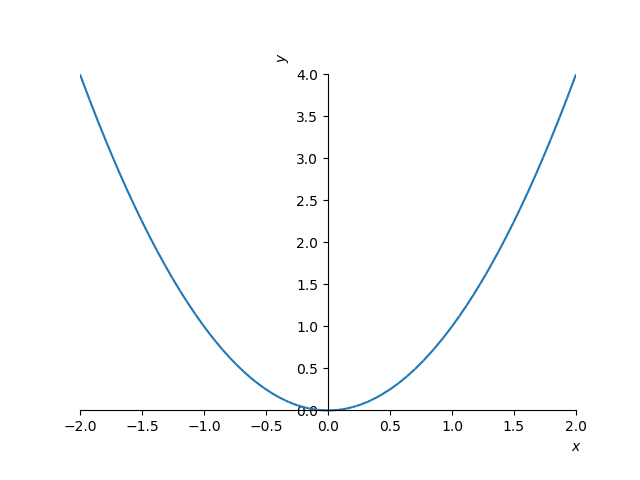
\includegraphics[width=0.7\textwidth]{./cap_funcao/dados/fig_ex_grafico/fig_ex_grafico_x2}
      \caption{Esboço do gráfico de $f(x)=x^2$.}
    \end{figure}

    \ifispython
    Com o {\sympy}, podemos plotar este gráfico com o seguinte código.
    \begin{lstlisting}
      from sympy import *
      x = Symbol('x', real=True)
      plot(x**2, (x,-2, 2))
    \end{lstlisting}
    \fi

  \item $\displaystyle y=\frac{1}{x}$

    \begin{figure}[H]
      \centering
      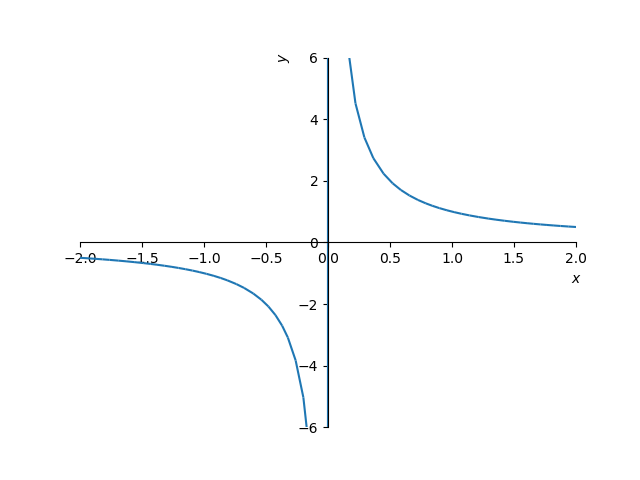
\includegraphics[width=0.7\textwidth]{./cap_funcao/dados/fig_ex_grafico/fig_ex_grafico_1x}
      \caption{Esboço do gráfico de $\displaystyle y = \frac{1}{x}$.}
    \end{figure}

    \ifispython
    Com o {\sympy}, podemos plotar este gráfico com o seguinte código
    \begin{lstlisting}
      from sympy import *
      x = Symbols('x', real=True)
      plot(1/x, (x,-2, 2), ylim=[-6, 6])
    \end{lstlisting}
    \fi

  \item $y = \sqrt{1-x^2}$

    \begin{figure}[H]
      \centering
      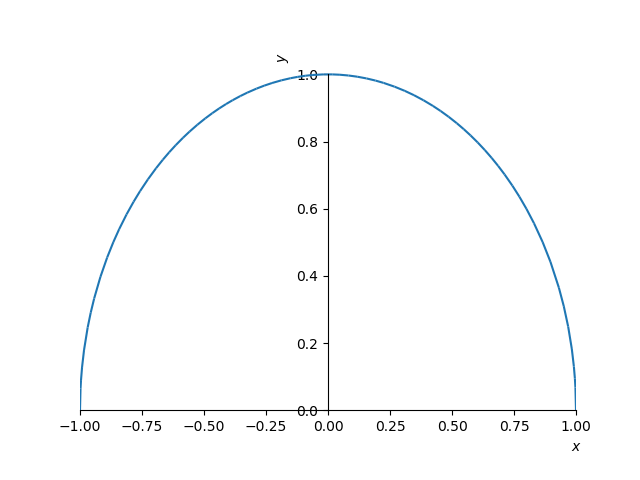
\includegraphics[width=0.7\textwidth]{./cap_funcao/dados/fig_ex_grafico/fig_ex_grafico_s1x2}
      \caption{Esboço do gráfico de $y = \sqrt{1-x^2}$.}
    \end{figure}

    \ifispython
    Com o {\sympy}, podemos plotar este gráfico com o seguinte código
    \begin{lstlisting}
      from sympy import *
      x = Symbols('x', real=True)
      plot(sqrt(1 - x**2), (x, -1, 1))
    \end{lstlisting}
    \fi
    
  \end{enumerate}
\end{ex}

\subsection{Categorias de funções}

\begin{flushright}
  [Vídeo] | [Áudio] | \href{https://phkonzen.github.io/notas/contato.html}{[Contatar]}
\end{flushright}

\subsubsection{Funções algébricas}

\emph{Funções algébricas} são funções definidas a partir de somas, subtrações, multiplicações, divisões ou extração de raízes de funções polinomiais. Funções polinomiais e as funções algébricas derivadas são estudas nas próximas seções.

\begin{ex}
  São exemplos de funções algébrigas:
  \begin{enumerate}[a)]
  \item $\displaystyle f(x) = 2$
  \item $\displaystyle g(x) = 2x - 1$
  \item $\displaystyle h(x) = 2 - x^3 + x$
  \item $\displaystyle f_1(u) = \frac{u^2 + 2u + 1}{u - 1}$
  \item $\displaystyle y = 2^z - \sqrt{z - 1}$
  \end{enumerate}
\end{ex}

\subsubsection{Funções transcendentes}

\emph{Funções transcendentes} são funções que não são algébricas. Como exemplos, temos as funções trigonométricas, exponencial e logarítmica, as quais são introduzidas nas próximas seções.

\begin{ex}
  São exemplos de funções transcendentes:
  \begin{enumerate}[a)]
  \item $\displaystyle f(x) = e^{-x^2}$
  \item $\displaystyle y = \log_2(2x - 1)$
  \item $\displaystyle g(v) = \sen(v) - \cos(v)$
  \item $\displaystyle h(u) = \arctg(u)$
  \end{enumerate}
\end{ex}

\subsubsection{Funções definidas por partes}

\emph{Funções definidas por partes} são funções definidas por diferentes expressões matemáticas em diferentes partes de seu domínio.

Um exemplo fundamental de função definida por partes é a \emph{função valor absoluto}\footnote{Esta função também pode ser definida por $|x| = \sqrt{x^2}$.}
\begin{equation}
  |x| = \left\{
    \begin{array}{ll}
      x &, x\leq 0\\
      -x &, x<0
    \end{array}
\right.
\end{equation}
Vejamos o esboço do seu gráfico dado na Figura \ref{fig:cap_funcao_funabs}.

\begin{figure}[H]
  \centering
  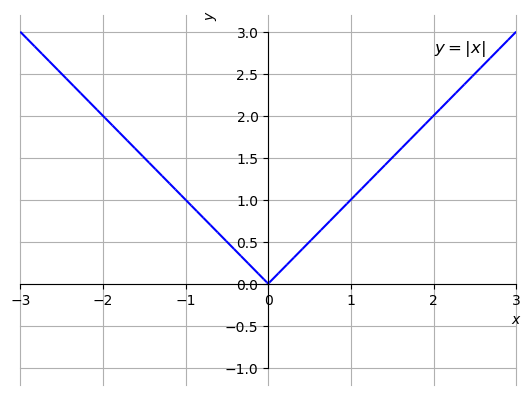
\includegraphics[width=0.7\textwidth]{./cap_funcao/dados/fig_cap_funcao_funabs/fig_cap_funcao_funabs}
  \caption{Esboço do gráfico da função valor absoluto $y=|x|$.}
  \label{fig:cap_funcao_funabs}
\end{figure}

\ifispython
Com o {\sympy}, a função valor absoluto é definida por \lstinline!abs()! ou \lstinline!Abs()!. Por exemplo, temos 
\begin{lstlisting}
  In : from sympy import *
  In : abs(-1)
  Out: 1
\end{lstlisting}
Use o {\sympy} para plotar o gráfico da função valor absoluto! Verifique com a Figura \ref{fig:cap_funcao_funabs}.
\fi

\subsection*{Exercícios}

\begin{flushright}
  [Vídeo] | [Áudio] | \href{https://phkonzen.github.io/notas/contato.html}{[Contatar]}
\end{flushright}

\begin{exer}
  Determine o domínio e a imagem da função identidade, i.e. $f(x) = x$. Então, faça o esboço de seu gráfico.
\end{exer}
\begin{resp}
  Domínio: $\mathbb{R}$; Imagem: $\mathbb{R}$
\end{resp}

\begin{exer}
  Determine o domínio e a imagem da função $f(x) = x^2 + 1$. Então, faça o esboço de seu gráfico.
\end{exer}
\begin{resp}
  Domínio: $\mathbb{R}$; Imagem: $[1, \infty)$.
\end{resp}

\begin{exer}
  Determine o domínio e a imagem da função $f(x) = 1 - x^2$. Então, faça o esboço de seu gráfico.
\end{exer}
\begin{resp}
  Domínio: $\mathbb{R}$; Imagem: $(-\infty, 1]$.
\end{resp}

\begin{exer}
  Determine o domínio e a imagem da função
  \begin{equation}
    h(x) = \frac{1}{x-1} - 2.
  \end{equation}
  Então, faça o esboço de seu gráfico.
\end{exer}
\begin{resp}
  Domínio: $(-\infty, 1)\cup (1, \infty)$; Imagem: $(-\infty, -2)\cup (-2, \infty)$.
\end{resp}

\begin{exer}
  Determine o domínio e a imagem da função valor absoluto.
\end{exer}
\begin{resp}
  Domínio: $\mathbb{R}$; Imagem: $[0, \infty)$.
\end{resp}

\section{Função afim}\label{cap_funcao_sec_funafim}

\begin{flushright}
  [Vídeo] | [Áudio] | \href{https://phkonzen.github.io/notas/contato.html}{[Contatar]}
\end{flushright}

Uma \emph{função afim} é uma função da forma
\begin{equation}
f(x) = mx + b,
\end{equation}
sendo $m$ e $b$ parâmetros\footnote{números reais.} dados. O parâmetro $m$ é chamado de \pmb{coeficiente angular} e o parâmetro $b$ é chamado de \pmb{coeficiente constante}\footnote{Mais corretamente, coeficiente do termo constante.}.

Quando $m=0$, temos uma \emph{função constante} $f(x) = b$. Esta tem domínio $(-\infty, \infty)$ e imagem $\{b\}$. Quando $b=0$, temos uma \pmb{função linear} $f(x)=mx$, cujo domínio é $(-\infty, \infty)$ e imagem é $(-\infty, \infty)$.

De forma geral, toda função linear com $m\neq 0$ tem $(-\infty, \infty)$ como domínio e imagem.

\begin{ex}\label{ex:funafim}
  A Figura \ref{fig:ex_funafim} mostra esboços dos gráficos das funções afins $f(x)=-5/2$, $f(x)=2$ e $f(x)=2x-1$.
  
  \begin{figure}[H]
    \centering
    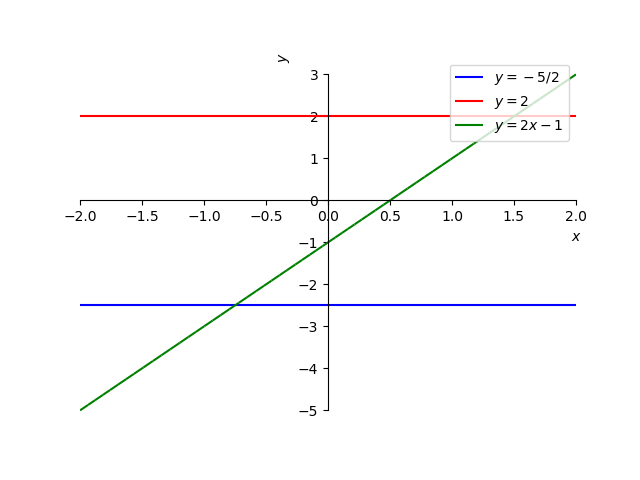
\includegraphics[width=0.7\textwidth]{./cap_funcao/dados/fig_ex_funafim/fig_ex_funafim}
    \caption{Esboços dos gráficos das funções afins $y=-5/2$, $y=2$ e $y=2x-1$ discutidas no Exemplo \ref{ex:funafim}.}
    \label{fig:ex_funafim}
  \end{figure}

  \ifispython
  Com o {\sympy}, podemos plotar o gráfico mostrado na Figura \ref{fig:ex_funafim} com o seguinte código:
  \begin{lstlisting}
    from sympy import *
    x = Symbol('x')
    p = plot(-5/2, (x,-2,2), line_color="blue", show=False)
    q = plot(2, (x,-2,2), line_color="red", show=False)
    p.extend(q)
    q = plot(2*x-1, (x,-2,2), line_color="green", show=False)
    p.extend(q)
    p[0].label = "$y=-5/2$"
    p[1].label = "$y=2$"
    p[2].label = "$y=$"
    p.legend = True
    p.show() 
  \end{lstlisting}
  \fi
\end{ex}

O lugar geométrico do gráfico de uma função afim é uma reta (ou linha). O coeficiente angular $m$ controla a \emph{inclinação da reta} em relação ao eixo $x$\footnote{eixo das abscissas}. Quando $m=0$, temos uma reta horizontal. Quando $m>0$ temos uma reta com inclinação positiva (crescente) e, quando $m<0$ temos uma reta com inclinação negativa.

\begin{ex}\label{ex:funlinear}
  A Figura \ref{fig:ex_funlinear} mostra esboços dos gráficos das funções lineares $f_1(x)=\frac{1}{2}x$, $f_2(x) = x$, $f_3(x) = 2x$, $f_4(x)=-2x$, $f_5(x)=-x$ e $f_6(x)=-\frac{1}{2}x$.
  
  \begin{figure}[H]
    \centering
    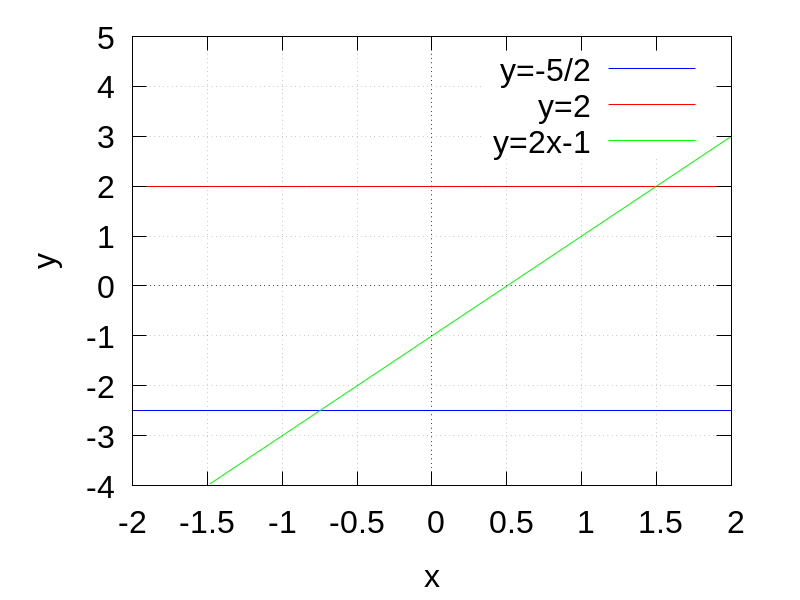
\includegraphics[width=0.7\textwidth]{./cap_funcao/dados/fig_ex_funlinear/fig_ex_funlinear}
    \caption{Esboços dos gráficos das funções lineares discutidas no Exemplo \ref{ex:funlinear}.}
    \label{fig:ex_funlinear}
  \end{figure}

  \ifispython
  Verifique, plotando os gráficos com o {\sympy}!
\end{ex}

\begin{figure}[H]
  \centering
  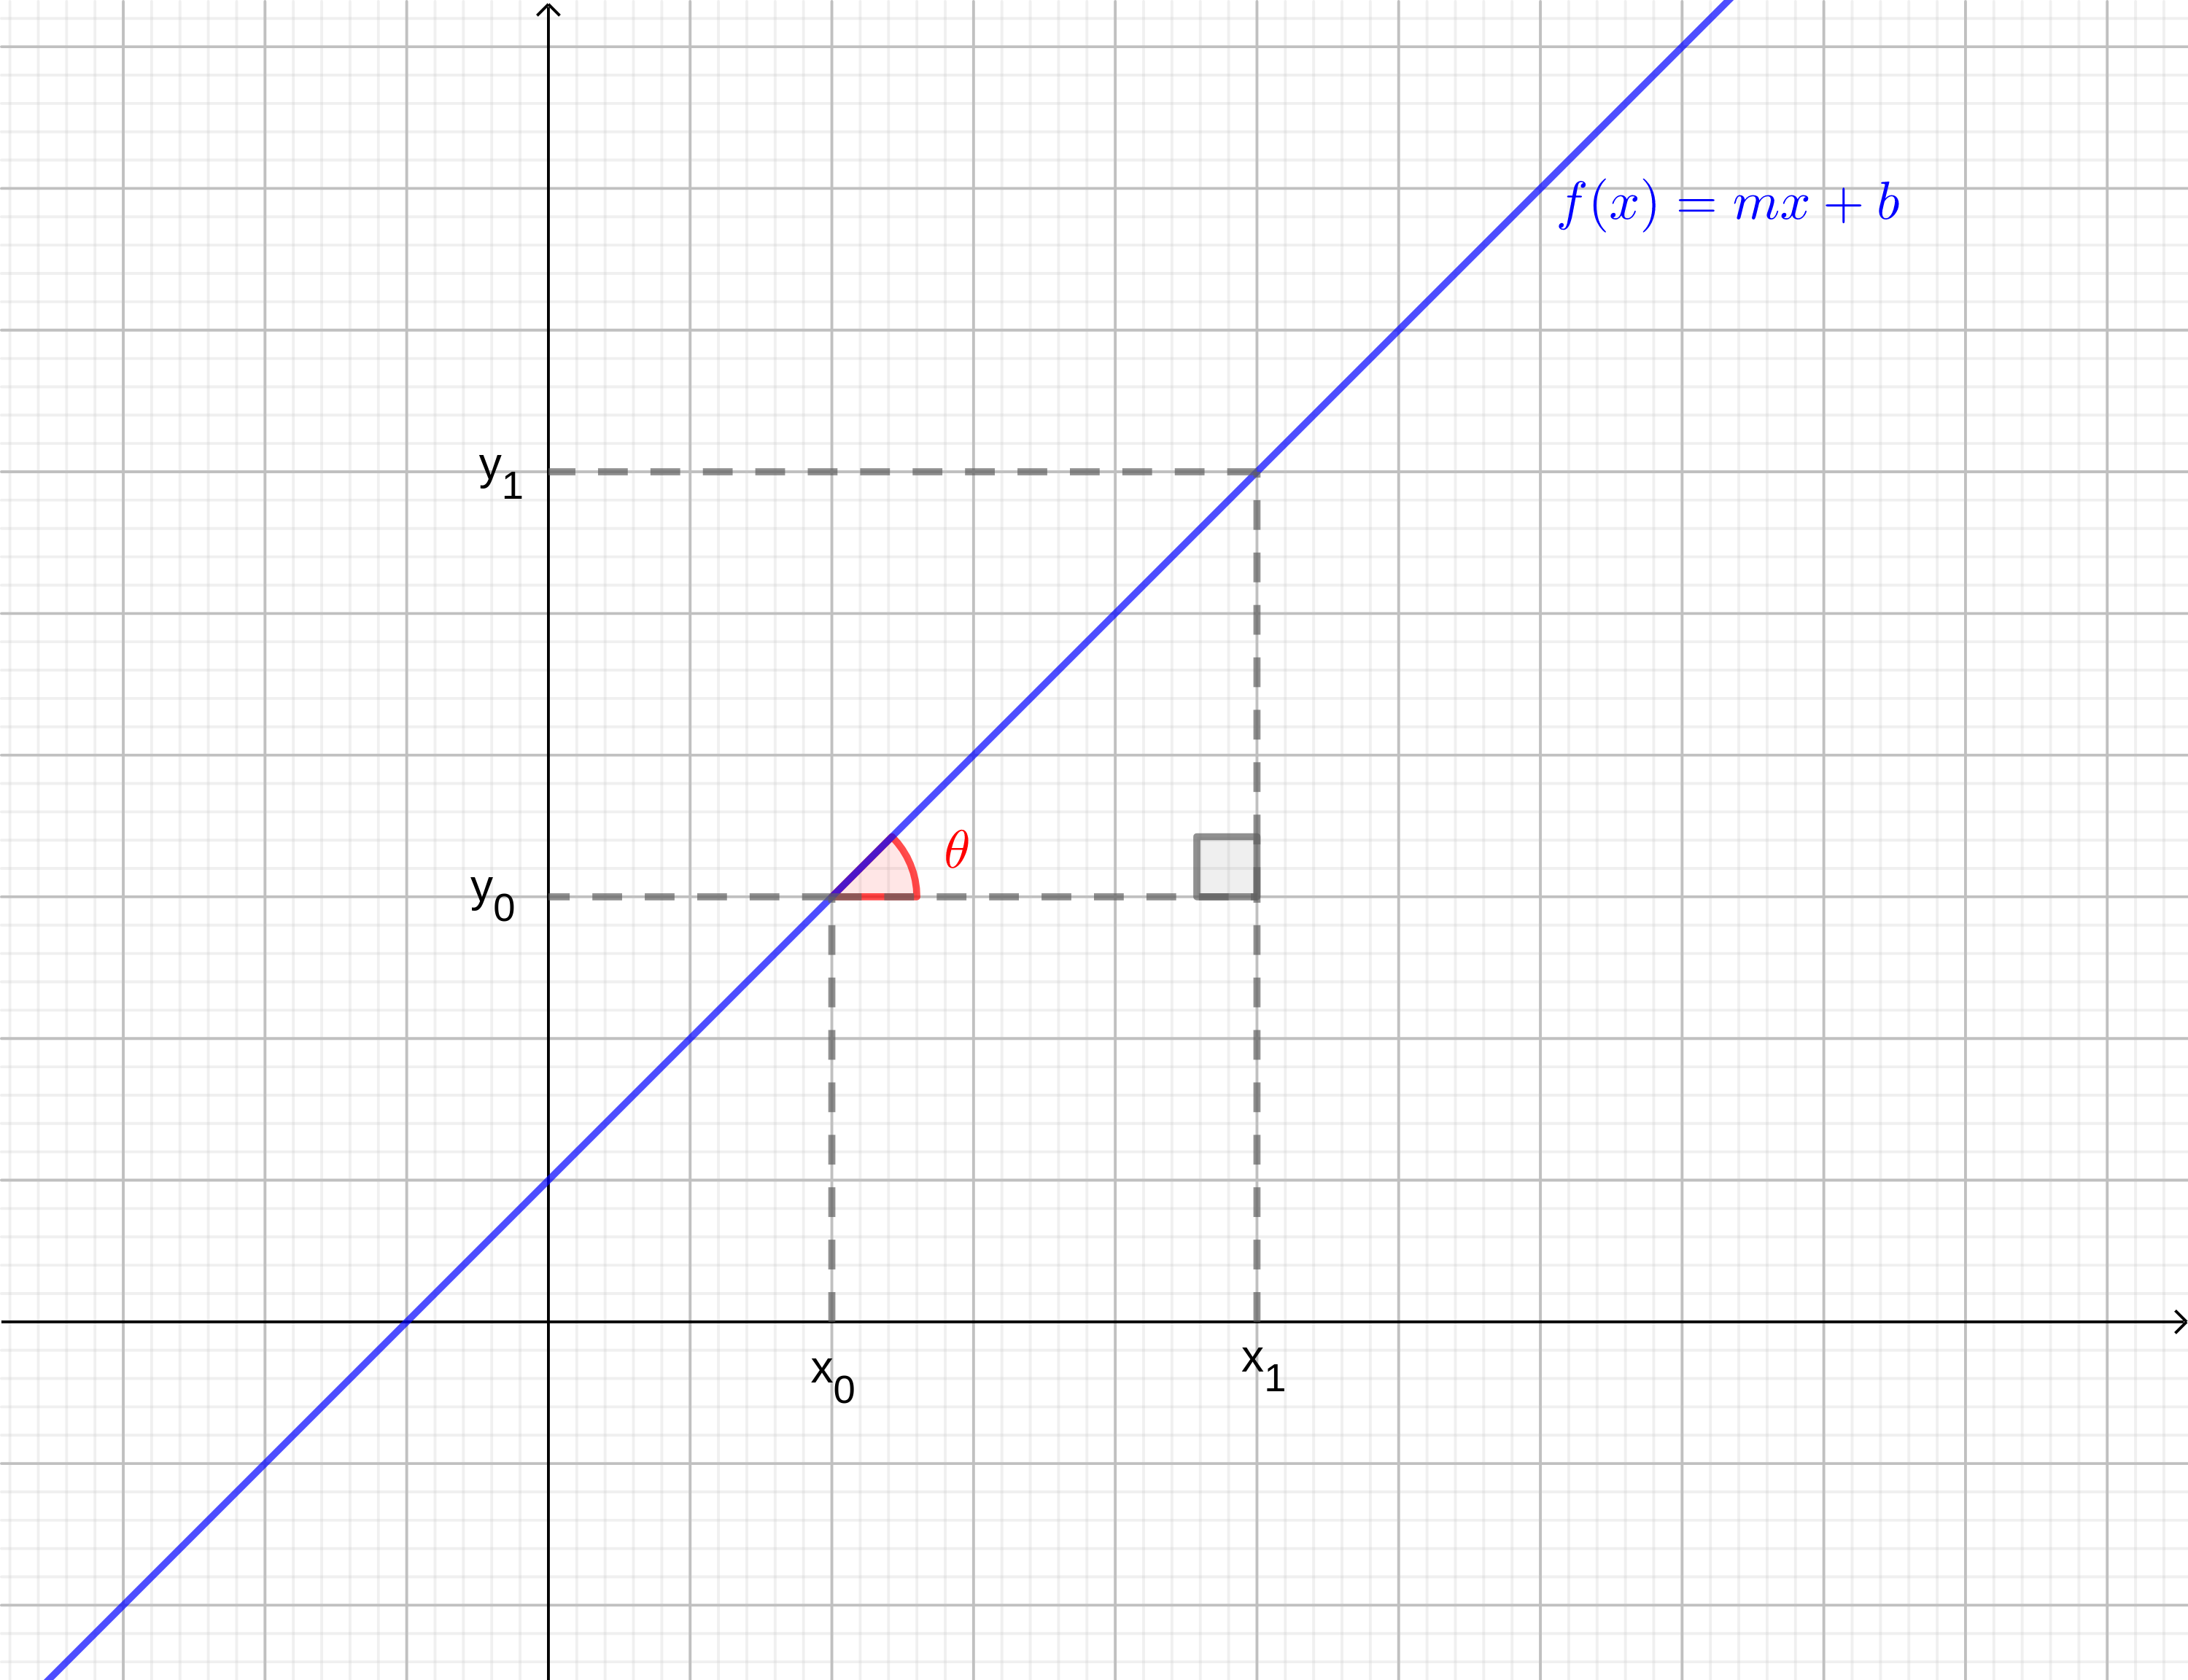
\includegraphics[width=0.7\textwidth]{./cap_funcao/dados/fig_declividade/fig_declividade}
  \caption{Declividade e o coeficiente angular.}
  \label{fig:declividade}
\end{figure}

A inclinação de uma reta é, normalmente, medida pelo \emph{ângulo de declividade} (veja a Figura \ref{fig:declividade}). Para definirmos este ângulo, sejam $(x_0, y_0)$ e $(x_1, y_1)$, $x_0<x_1$, pontos sobre uma dada reta, gráfico da função afim $f(x)=mx+b$. O ângulo de declividade (ou, simplesmente, a declividade) da reta é, por definição, o ângulo formado pelo segmento que parte de $(x_0, y_0)$ e termina em $(x_1, y_0)$ e o segmento que parte de $(x_0, y_0)$ e termina em $(x_1, y_1)$. Denotando este ângulo por $\theta$, temos
\begin{align}
  \tg\theta &= \frac{\text{cateto oposto}}{\text{cateto adjacente}}\\
            &= \frac{y_1-y_0}{x_1-x_0}\\
            &= \frac{mx_1+b-(mx_0+b)}{x_1-x_0}\\
            &= m,
\end{align}
o que justifica chamar $m$ de coeficiente angular.

Quaisquer dois pontos $(x_0, y_0)$ e $(x_1, y_1)$, com $x_0\neq x_1$, determinam uma única função afim (reta) que passa por estes pontos. Para encontrar a expressão desta função, basta resolver o seguinte sistema linear
\begin{align}
  mx_0 + b &= y_0\\
  mx_1 + b &= y_1
\end{align}
Subtraindo a primeira equação da segunda, obtemos
\begin{gather}
  m(x_0-x_1) = y_0-y_1\\
  m = \frac{y_0-y_1}{x_0-x_1}
\end{gather}
Daí, substituindo o valor de $m$ na primeira equação do sistema, obtemos
\begin{gather}
  \frac{y_0-y_1}{x_0-x_1}x_0 + b = y_0 \\
  b = -\frac{y_0-y_1}{x_0-x_1}x_0 + y_0
\end{gather}
Ou seja, a expressão da função linear (\emph{equação da reta}) que passa pelos pontos $(x_0, y_0)$ e $(x_1, y_1)$ é
\begin{equation}\label{eq:funafim_eq}
  y = \underbrace{\frac{y_0-y_1}{x_0-x_1}}_{m}(x-x_0) + y_0.
\end{equation}

\begin{ex}
  Vamos traçar o esboço da reta que representa o gráfico da função afim $f(x) = -x-1$. Para tanto, basta traçarmos a reta que passa por quaisquer dois pontos distintos de seu gráfico. Por exemplo, no caso da função $f(x) = -x -1$, temos
  \begin{center}
  \begin{tabular}[H]{r|c}
    $x$ & $y = -x-1$\\\hline
    -1  & 0\\
    1   & -2\\\hline
  \end{tabular}
\end{center}
Assim sendo, marcamos os pontos $(-1, 0)$ e $(1, -2)$ em um plano cartesiano e traçamos a reta que passa por eles. Veja a Figura \ref{fig:exeresol_funafim_grafico}.

\begin{figure}[H]
  \centering
  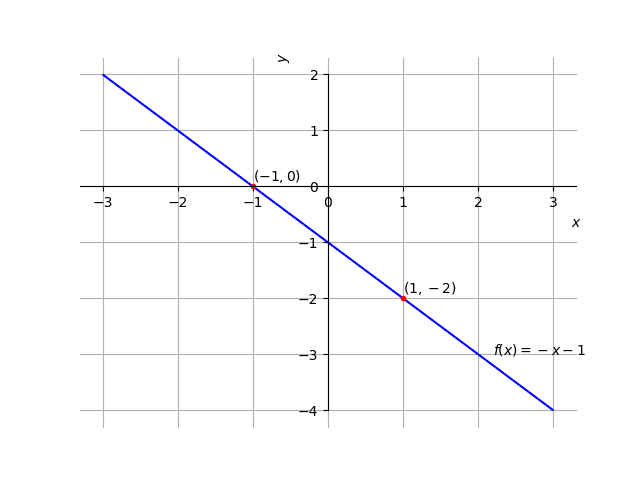
\includegraphics[width=0.7\textwidth]{./cap_funcao/dados/fig_exeresol_funafim_grafico/fig_exeresol_funafim_grafico}
  \caption{Esboço do gráfico da função afim $f(x)=-x-1$.}
  \label{fig:exeresol_funafim_grafico}
\end{figure}

\ifispython
Plote o gráfico com o {\sympy} e compare com o seu esboço!
\fi
\end{ex}

\begin{ex}
  Vamos determinar a função afim $f(x) = mx + b$, cujo gráfico contém os pontos $(1, -1)$ e $(2, 1)$. Para tanto, vamos usar \eqref{eq:funafim_eq}. Tomamos
  \begin{gather}
    (x_0, y_0) = (1, -1)\\
    (x_1, y_1) = (2, 1)
  \end{gather}
  Então, substituindo em \eqref{eq:funafim_eq} temos
  \begin{equation}
    m = \frac{y_1 - y_0}{x_1 - x_0} = \frac{1 - (-1)}{2 - 1} = 2.
  \end{equation}
  De \eqref{eq:funafim_eq}, temos
  \begin{align}
    f(x) &= m(x-x_0) + y_0\\
         &= 2(x - 1) + (-1) \\
         &= 2x -3.
  \end{align}
  Ou seja, a função afim desejada é $f(x) = 2x - 3$.

  \ifispython
  Com o {\sympy}, podemos resolver este exercício utilizando o seguinte código:
\begin{verbatim}
from sympy import *
x = Symbol('x')
x0 = 1
y0 = -1
x1 = 2
y1 = 1
m = (y1-y0)/(x1-x0)
f = Lambda(x, m*(x-x0) + y0)
print(f"f(x) = {f(x)}")
\end{verbatim}
  \fi
\end{ex}

\subsection*{Exercícios}

\begin{flushright}
  [Vídeo] | [Áudio] | \href{https://phkonzen.github.io/notas/contato.html}{[Contatar]}
\end{flushright}

\begin{exer}
  Determine o domínio e a imagem de cada uma das seguintes funções afins:
  \begin{enumerate}[a)]
  \item $f(x) = -100x + 1$
  \item $y = -\pi$
  \item $h(v) = 2 + x$
  \end{enumerate}
\end{exer}
\begin{resp}
  a) $D=\mathbb{R}$; $I=\mathbb{R}$; b) $D=\mathbb{R}$, $I=\{\pi\}$; c) $D=\mathbb{R}$; $I=\mathbb{R}$
\end{resp}

\begin{exer}
  Faça um esboço do gráfico de cada uma das seguintes funções:
  \begin{enumerate}[a)]
  \item $f_1(x) = x$
  \item $f_2(x) = -x$
  \item $f_3(x) = x-1$
  \item $f_4(x) = -x+1$
  \end{enumerate}
\end{exer}

\begin{exer}
  Determine a função afim $f(x)=mx+b$, cujo gráfico contém os pontos $(-2, 1)$ e $(0, -2)$.
\end{exer}
\begin{resp}
  $f(x) = -\frac{3}{2}x - 2$
\end{resp}

\begin{exer}
  Verifique se as retas $y = -x - 1$ e $y = 2x - 3$ se interceptam e, caso afirmativo, determine o ponto de interseção.
\end{exer}
\begin{resp}
  $(2/3,-5/3)$
\end{resp}

\begin{exer}
  Determine o ponto de interseção dos gráficos das funções afins $f(x) = 2x + 1$ e $g(x) = 2x -1$.
\end{exer}
\begin{resp}
  não há
\end{resp}



\section{Função potência}\label{cap_funcao_sec_funpot}

\begin{flushright}
  [Vídeo] | [Áudio] | \href{https://phkonzen.github.io/notas/contato.html}{[Contatar]}
\end{flushright}

Uma função da forma $f(x)=x^n$, onde $n\neq 0$ é uma constante, é chamada de \emph{função potência}.

Funções potências têm comportamentos característicos, conforme o valor de $n$. Quando $n$ é um inteiro positivo ímpar, seu domínio e sua imagem são $(-\infty, \infty)$. Veja a Figura \ref{fig:funpot_impar}.

\begin{figure}[H]
  \centering
  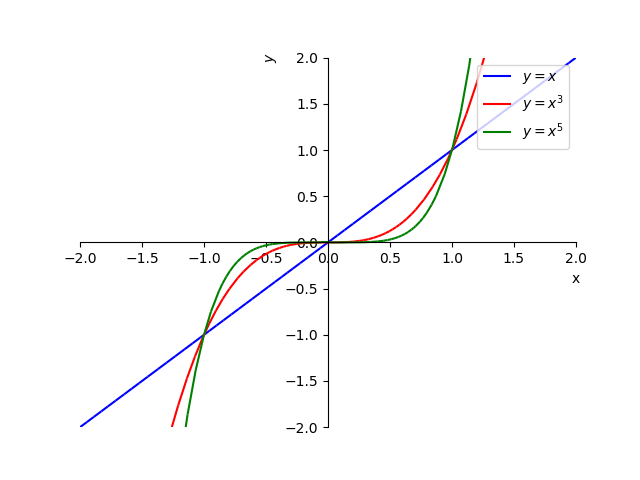
\includegraphics[width=0.7\textwidth]{./cap_funcao/dados/fig_funpot_impar/fig_funpot_impar}
  \caption{Esboços dos gráficos das funções potências $y=x$, $y=x^3$ e $y=x^5$.}
  \label{fig:funpot_impar}
\end{figure}

Funções potências com $n$ positivo par estão definidas em toda parte e têm imagem $[0, \infty)$. Veja a Figura \ref{fig:funpot_par}.

\begin{figure}[H]
  \centering
  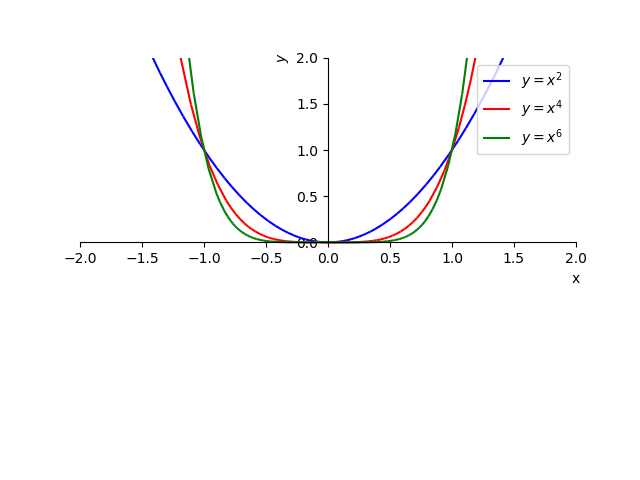
\includegraphics[width=0.7\textwidth]{./cap_funcao/dados/fig_funpot_par/fig_funpot_par}
  \caption{Esboços dos gráficos das funções potências $y=x^2$, $y=x^4$ e $y=x^6$.}
  \label{fig:funpot_par}
\end{figure}

Funções potências com $n$ inteiro negativo ímpar não são definidas em $x=0$, tendo domínio e imagem igual a $(-\infty, 0)\cup (0, \infty)$. Também, quando $n$ inteiro negativo par, a função potência não está definida em $x=0$, tem domínio $(-\infty, 0)\cup (0, \infty)$, mas imagem $(0, \infty)$. Veja a Figura \ref{fig:funpot_negativo}.

\begin{figure}[H]
  \centering
  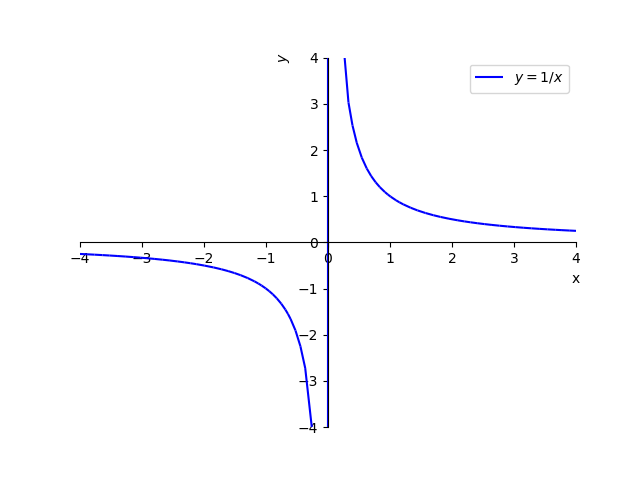
\includegraphics[width=0.5\textwidth]{./cap_funcao/dados/fig_funpot_negativo/fig_funpot_negativo_impar}~
    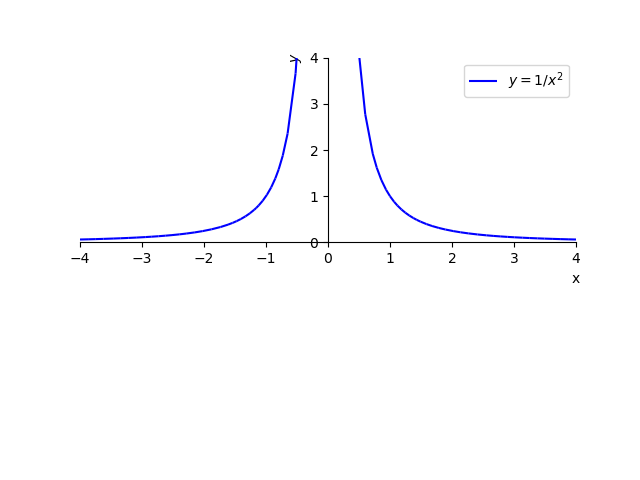
\includegraphics[width=0.5\textwidth]{./cap_funcao/dados/fig_funpot_negativo/fig_funpot_negativo_par}
  \caption{Esboços dos gráficos das funções potências $y=1/x$ (esquerda), $y=1/x^2$ (direita).}
  \label{fig:funpot_negativo}
\end{figure}

Há, ainda, comportamentos característicos quando $n=1/2$, $1/3$, $3/2$ e $2/3$. Veja a Figura \ref{fig:funpot_racional}.

\begin{figure}[H]
  \centering
  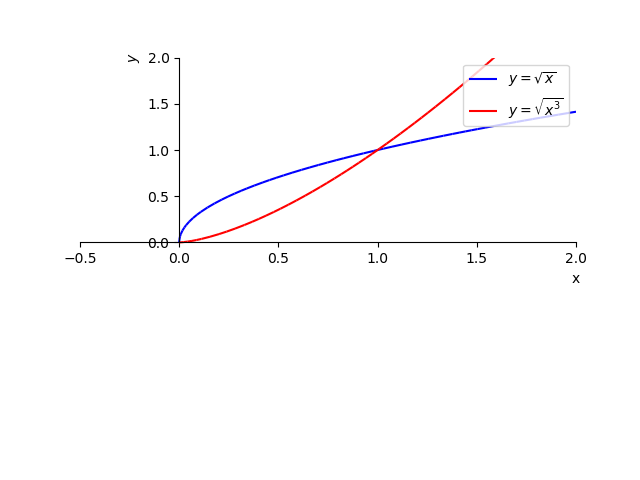
\includegraphics[width=0.5\textwidth]{./cap_funcao/dados/fig_funpot_racional/fig_funpot_racional_par}~
    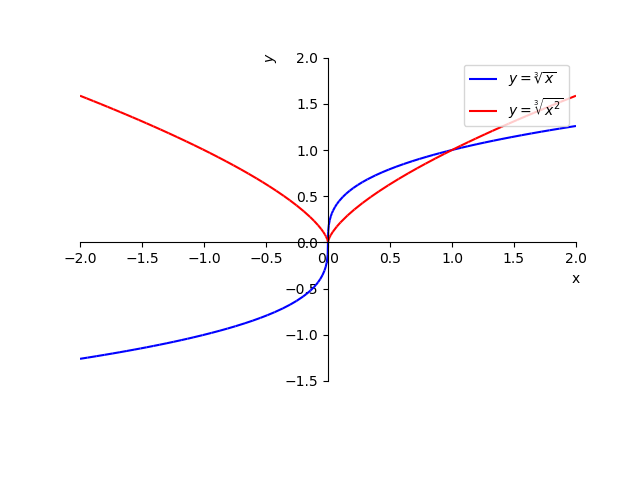
\includegraphics[width=0.5\textwidth]{./cap_funcao/dados/fig_funpot_racional/fig_funpot_racional_impar}
  \caption{Esboços dos gráficos das funções potências. Esquerda $y=\sqrt{x}$ e $y=\sqrt{x^3}$. Direita: $y=\sqrt[3]{x}$ e $y=\sqrt[3]{x^2}$.}
  \label{fig:funpot_racional}
\end{figure}


\subsection*{Exercícios resolvidos}

\begin{flushright}
  [Vídeo] | [Áudio] | \href{https://phkonzen.github.io/notas/contato.html}{[Contatar]}
\end{flushright}

\begin{exeresol}\label{exeresol:funpot_graf}
  Determine o domínio e faça um esboço do gráfico de cada uma das seguintes funções:
  \begin{enumerate}[a)]
  \item $\displaystyle f(x) = x^{5/2}$;
  \item $\displaystyle g(x) = x^{5/3}$.
  \end{enumerate}
\end{exeresol}
\begin{resol}
  \begin{enumerate}[a)]
  \item Vamos analisar a função $f(x) = x^{5/2}$. Como $x^{5/2} = \sqrt{x^5}$ e não existe a raiz quadrada de número negativo, temos que $x^5$ deve ser não negativo. Daí, $x$ deve ser não negativo. Logo, o domínio de $f(x) = x^{5/2}$ é $[0, \infty)$. Veja o esboço desta função na Figura \ref{fig:exeresol_funpot_graf_a}.

    \begin{figure}[H]
      \centering
      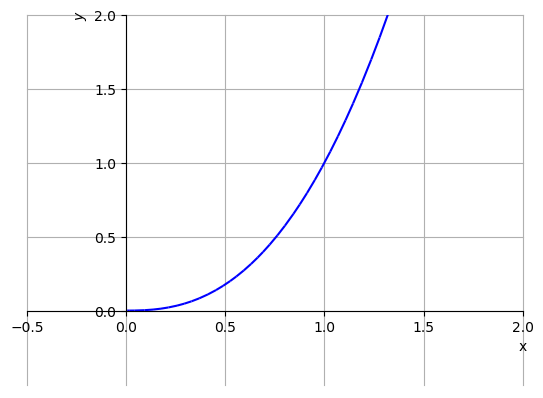
\includegraphics[width=0.5\textwidth]{./cap_funcao/dados/fig_exeresol_funpot_graf/fig_exeresol_funpot_graf_a}
      \caption{Esboço do gráfico de $f(x) = x^{5/2}$.}
      \label{fig:exeresol_funpot_graf_a}
    \end{figure}

    \ifispython
    Para plotar o gráfico de $f(x)$ com o \sympy, basta digitar, por exemplo:
\begin{verbatim}
plot(x**(5/2),(x,0,2))
\end{verbatim}
    \fi
  \item Vamos analisar a função $g(x) = x^{5/3}$. Como $x^{5/3} = \sqrt[3]{x^5}$, não temos restrição sobre os valores de $x$. Logo, o domínio da função $g$ é $(-\infty, \infty)$. Veja o esboço desta função na Figura \ref{fig:exeresol_funpot_graf_b}.

    \begin{figure}[H]
      \centering
      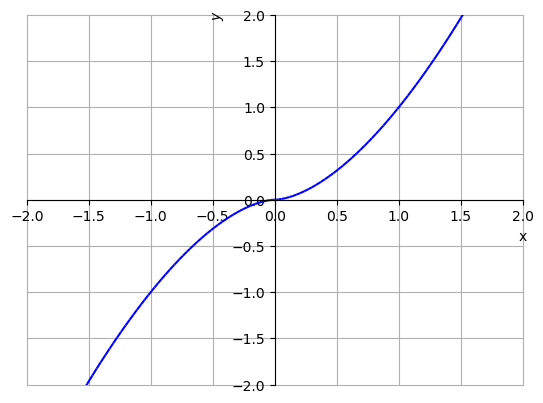
\includegraphics[width=0.5\textwidth]{./cap_funcao/dados/fig_exeresol_funpot_graf/fig_exeresol_funpot_graf_b}
      \caption{Esboço do gráfico de $g(x) = x^{5/3}$.}
      \label{fig:exeresol_funpot_graf_b}
    \end{figure}

    \ifispython
    Para plotar o gráfico de $g(x)$ com o \sympy, digitamos:
\begin{verbatim}
p = plot(x**(5/3),(x,0,2),line_color="blue",show=False)
q = plot(-(-x)**(5/3),(x,-2,0),line_color="blue",show=False)
p.extend(q)
p.show()
\end{verbatim}
    Você sabe o porquê não pode-se usar, simplesmente, o seguinte comando?
\begin{verbatim}
plot(x**(5/3),(x,-2,2))
\end{verbatim}
    \fi
  \end{enumerate}
\end{resol}

\begin{exeresol}\label{exeresol:funpot_intersep}
  Determine a equação da reta que passa pelos pontos de interseção dos gráficos das funções $f(x) = 1/x$ e $g(x) = \sqrt[3]{x}$.
\end{exeresol}
\begin{resol}
  Para determinarmos a reta precisamos, antes, dos pontos de interseção. As funções se interceptam nos pontos de abscissa $x$ tais que
  \begin{align}
    f(x) = g(x) &\Rightarrow \frac{1}{x} = \sqrt[3]{x}\\
                &\Rightarrow 1 = x\sqrt[3]{x}\\
                &\Rightarrow 1 = x\cdot x^{\frac{1}{3}}\\
                &\Rightarrow x^{1+\frac{1}{3}} = 1\\
                &\Rightarrow x^{\frac{4}{3}} = 1\\
                &\Rightarrow x^4 = \sqrt[3]{1}\\
                &\Rightarrow x^4 = 1\\
                &\Rightarrow x_0 = -1\quad\text{ou}\quad x_1=1.
  \end{align}
  Ou seja, os gráficos se interceptam nos pontos de abscissas $x_0 = -1$ e $x_1 = 1$. Veja o esboço dos gráficos das funções na Figura \ref{fig:exeresol_funpot_intersep}. Agora, podemos usar qualquer uma das funções para obter as ordenadas dos pontos de interseção. Usando $f(x)$, temos
  \begin{equation}
    (x_0, y_0) = (x_0, f(x_0)) = (-1, -1)\quad\text{e}\quad (x_1, y_1) = (x_1, f(x_1)) = (1, 1).
  \end{equation}

  \begin{figure}[H]
    \centering
    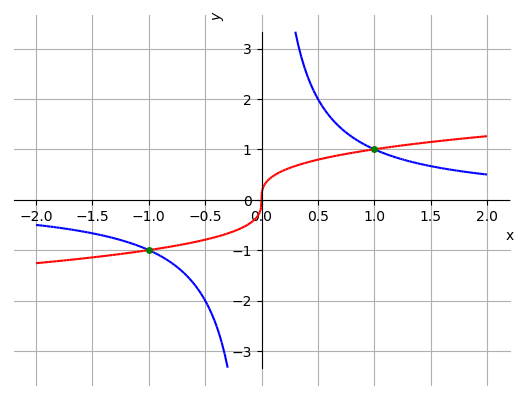
\includegraphics[width=0.5\textwidth]{./cap_funcao/dados/fig_exeresol_funpot_intersep/fig_exeresol_funpot_intersep}
    \caption{Interseção dos gráficos das funções $f(x) = 1/x$ (azul) e $g(x) = \sqrt[3]{x}$ (vermelho).}
    \label{fig:exeresol_funpot_intersep}
  \end{figure}

  Agora, basta determinarmos a equação da reta que passa pelos pontos $(x_0, y_0) = (-1, -1)$ e $(x_1, y_1) = (1, 1)$. De \eqref{eq:funafim_eq}, temos que a equação da reta é tal que
  \begin{align}
    y = \frac{y_1-y_0}{x_1-x_0}(x-x_0)+y_0 &\Rightarrow y = \frac{1-(-1)}{1-(-1)}(x-(-1))+(-1)\\
                                           &\Rightarrow y = x+1-1 \Rightarrow y = x.
  \end{align}
  Ou seja, a que passa pelos pontos de interseção dos gráficos das funções $f(x)$ e $g(x)$ tem equação $y = x$.

  \ifispython
  Os seguintes comandos, mostrar como podemos resolver este problema usando o \sympy\footnote{Veja a Observaçao \ref{cap_funcao_python}.}:
\begin{verbatim}
f = lambda x: 1/x
# x nao negativo
g1 = lambda x: cbrt(x)
# x negativo
g2 = lambda x: -cbrt(-x)

x0 = solve(f(x)-g2(x))[0]
x1 = solve(f(x)-g1(x))[0]

y0 = f(x0)
y1 = f(x1)

print('y = ',(y1-y0)/(x1-x0)*(x-x0)+y0)
\end{verbatim}
  \fi
\end{resol}

\subsection*{Exercícios}

\begin{flushright}
  [Vídeo] | [Áudio] | \href{https://phkonzen.github.io/notas/contato.html}{[Contatar]}
\end{flushright}

\begin{exer}
  Determine o domínio, a imagem e faça um esboço do gráfico de cada uma das seguintes funções:
  \begin{enumerate}[a)]
  \item $f(x) = x^7$;
  \item $g(x) = x^8$.
  \end{enumerate}
\end{exer}
\begin{resp}
  a) domínio: $(-\infty, \infty)$; imagem: $(-\infty, \infty)$. b) domínio: $(-\infty, \infty)$; imagem: $[0, \infty)$. Dica: use o \href{https://www.sympygamma.com/}{SymPy Gamma} para verificar os esboços de seus gráficos.
\end{resp}

\begin{exer}
  Determine o domínio, a imagem e faça um esboço do gráfico de cada uma das seguintes funções:
  \begin{enumerate}[a)]
  \item $\displaystyle f(x) = \frac{1}{x^7}$;
  \item $\displaystyle g(x) = \frac{1}{x^8}$.
  \end{enumerate}
\end{exer}
\begin{resp}
  a) domínio: $(-\infty, \infty)\setminus\{0\}$; imagem: $(-\infty, \infty)\setminus\{0\}$. b) domínio: $(-\infty, \infty)\setminus\{0\}$; imagem: $(0, \infty)$. Dica: use o \href{https://www.sympygamma.com/}{SymPy Gamma} para verificar os esboços de seus gráficos.
\end{resp}

\begin{exer}
  Determine o domínio, a imagem e faça um esboço do gráfico de cada uma das seguintes funções:
  \begin{enumerate}[a)]
  \item $\displaystyle f(x) = \sqrt{x^2}$;
  \item $\displaystyle g(x) = \sqrt[3]{x^3}$.
  \end{enumerate}
\end{exer}
\begin{resp}
  a) domínio: $(-\infty, \infty)$; imagem: $[0, \infty)$. b) domínio: $(-\infty, \infty)$; imagem: $(-\infty, \infty)$. Dica: use o \href{https://www.sympygamma.com/}{SymPy Gamma} para verificar os esboços de seus gráficos.
\end{resp}


\section{Função polinomial}\label{cap_funcao_sec_funpoli}

\begin{flushright}
  [Vídeo] | [Áudio] | \href{https://phkonzen.github.io/notas/contato.html}{[Contatar]}
\end{flushright}

Uma \emph{função polinomial} (\emph{polinômio}) tem a forma
\begin{equation}
  p(x) = a_nx^n + a_{n-1}x^{n-1} + \cdots + a_1x + a_0,
\end{equation}
onde $a_i$ são coeficientes reais, $a_n\neq 0$ e $n$ é inteiro não negativo, este chamado de \emph{grau do polinômio}.

Polinômios são definidos em toda parte\footnote{Uma função é dita ser definida em toda parte quando seu domínio é $(\infty, \infty)$}. Polinômios de grau ímpar tem imagem $(-\infty, \infty)$. Entretanto, a imagem polinômios de grau par dependem de cada caso. Iremos estudar mais propriedades de polinômios ao longo do curso de cálculo. Veja a Figura \ref{fig:poli_graficos}.

\begin{figure}[H]
  \centering
  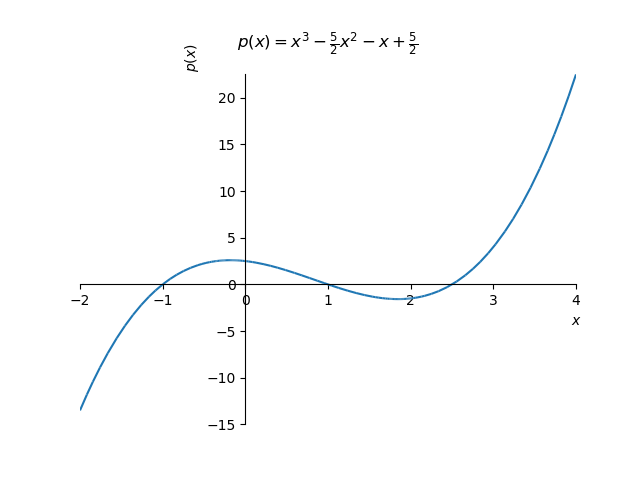
\includegraphics[width=0.5\textwidth]{./cap_funcao/dados/fig_poli_graficos/fig_poli_impar}~
    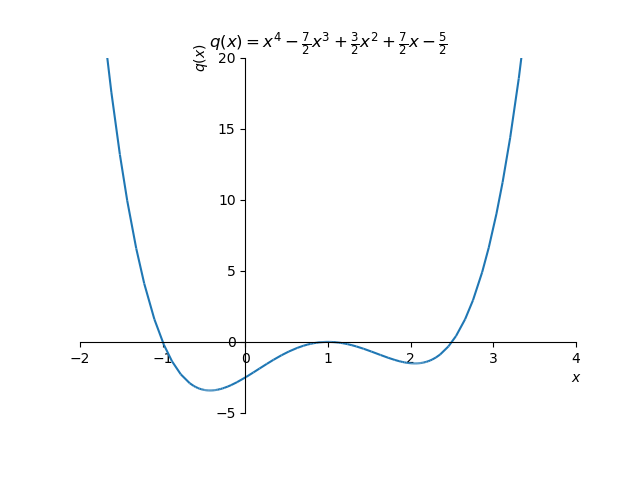
\includegraphics[width=0.5\textwidth]{./cap_funcao/dados/fig_poli_graficos/fig_poli_par}
  \caption{Esboços dos gráficos das funções polinomiais. Esquerda $p(x) = x^{3} - 2.5 x^{2} - 1.0 x + 2.5$. Direita: $q(x) = x^{4} - 3.5 x^{3} + 1.5 x^{2} + 3.5 x - 2.5$.}
  \label{fig:poli_graficos}
\end{figure}

Quando $n=0$, temos um polinômio de grau 0 (ou uma função constante). Quando $n=1$, temos um polinômio de grau 1 (ou, uma função afim). Ainda, quando $n=2$ temos uma \emph{função quadrática} (ou \emph{polinômio quadrático}) e, quando $n=3$, temos uma \emph{função cúbica} (ou \emph{polinômio cúbico}).

\subsection{Função quadrática}

\begin{flushright}
  [Vídeo] | [Áudio] | \href{https://phkonzen.github.io/notas/contato.html}{[Contatar]}
\end{flushright}

Os polinômios de grau 2 são, também, chamados de \pmb{funções quadráticas}, i.e. funções da forma
\begin{equation}
  f(x) = ax^2 + bx + c,
\end{equation}
onde $a$ é chamado de \pmb{coeficiente do termo quadrático}, $b$ o \pmb{coeficiente do termo linear} e $c$ o \pmb{coeficiente do termo constante}.

Os zeros de uma função quadrática podem ser calculados pela \pmb{fórmula de Bhaskara}
\begin{equation}\label{eq:Bhaskara}
  x_0, x_1 = \frac{-b \pm \sqrt{b^2 - 4ac}}{2a}.
\end{equation}


O esboço do gráfico de uma função quadrática é uma \pmb{parábola côncava para cima} quando $a > 0$ e, \pmb{côncava para baixo} quando $x < 0$. Veja a Figura \ref{fig:funquad_concavidade}.

\begin{figure}[H]
  \centering
  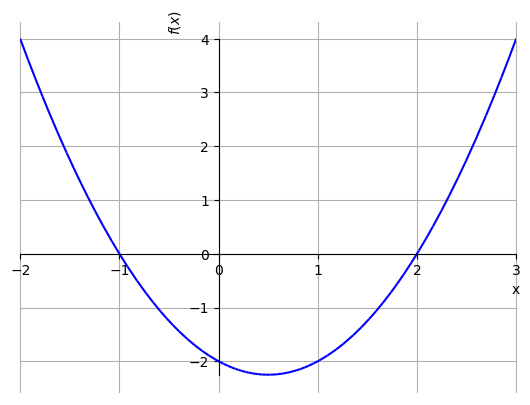
\includegraphics[width=0.5\textwidth]{./cap_funcao/dados/fig_funquad_concavidade/fig_funquad_concavidade_cima}~
    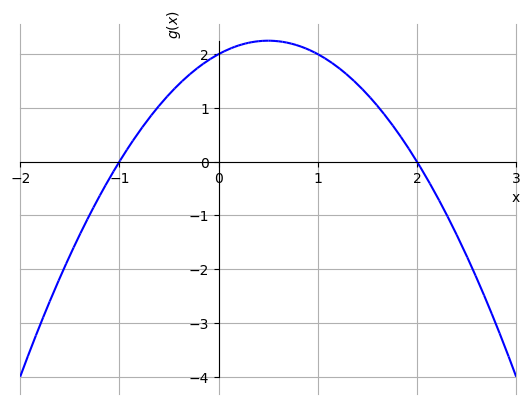
\includegraphics[width=0.5\textwidth]{./cap_funcao/dados/fig_funquad_concavidade/fig_funquad_concavidade_baixo}
  \caption{Esboço dos gráficos das funções quadráticas $f(x) = x^2-x-2$ (esquerda) e $g(x)=-x^2+x+2$ (direita).}
  \label{fig:funquad_concavidade}
\end{figure}

O \pmb{vértice} da função quadrática $f(x)$ com coeficiente quadrático positivo (com coeficiente quadrático negativo) é o ponto no qual ela atinge seu {\bf valor máximo (mínimo)} em todo o seu domínio natural. Quando $f$ têm zeros reais, o ponto de abscissa do vértice é o ponto médio entre os zeros $x_0$ e $x_1$ da função, i.e. o vértice $V = (x_v, y_v)$ é tal que
\begin{equation}
  x_v = \frac{x_0 + x_1}{2},\quad\text{e}\quad y_v = f(x_v). 
\end{equation}
O valor $x_v$ é a abscissa do ponto em que a função quadrática $f$ atinge o valor máximo (valor mínimo) $y_v$.


\subsection*{Exercícios resolvidos}

\begin{flushright}
  [Vídeo] | [Áudio] | \href{https://phkonzen.github.io/notas/contato.html}{[Contatar]}
\end{flushright}

\begin{exeresol}
  Determine os zeros do polinômio $f(x) = x^3-x^2-2x$.
\end{exeresol}
\begin{resol}
  Determinar os zeros da função $f$ significa entrar todos os valores de $x$ tais que $f(x)=0$ (estes são as abscissas dos pontos nos quais o gráfico de $f$ intersepta o eixo das abscissas). Temos
  \begin{align}
    f(x)=0 &\Rightarrow x^3-x^2-2x=0\\
           &\Rightarrow x(x^2-x-2)=0\\
           &\Rightarrow x=0\quad\text{ou}\quad x^2-x-2=0.
  \end{align}
  Então, usando a fórmula de Bhaskara \eqref{eq:Bhaskara} na equação $x^2-x-2=0$, obtemos
  \begin{align}
    x &= \frac{-b\pm\sqrt{b^2-4ac}}{2a} \\
      &= \frac{1\pm\sqrt{1-4\cdot 1\cdot (-2)}}{2}\\
      &= \frac{1\pm\sqrt{9}}{2}\\
      &= \frac{1\pm 3}{2}\\
      &= -1\quad\text{ou}\quad 2
  \end{align}
  Com isso, temos que os zeros da função $f$ ocorrem nos pontos $x_0 = -1$, $x_1=0$ e $x_2=2$.

  \ifispython
  Com o \sympy, podemos calcular os zeros da função $f$ com o seguinte comando:
\begin{verbatim}
solve(x**3-x**2-2*x)
\end{verbatim}
  \fi
\end{resol}

\begin{exeresol}
  Determine o valor mínimo da função $f(x) = x^2 - x - 2$.
\end{exeresol}
\begin{resol}
  Como $f$ é uma função quadrática com coeficiente quadrático positivo, temos que seu gráfico é uma parábola côncava para cima. Logo, $f$ atinge seu valor mínimo no seu vértice. Por sorte, os zeros de $f$ são $x_0 = -1$ e $x_1 = 2$. Logo, o vértice tem abscissa
  \begin{equation}
    x = \frac{x_0 + x_1}{2} = \frac{1}{2}.
  \end{equation}
  Ou seja, a abscissa do ponto de mínimo de $f$ é $1/2$ e seu valor mínimo é
  \begin{equation}
    f\left(\frac{1}{2}\right) = \left(\frac{1}{2}\right)^2-\frac{1}{2}-2 = \frac{1-2-8}{4} = -\frac{9}{4}.
  \end{equation}

  \ifispython
  Podemos resolver este exercício com o seguinte código \sympy:
\begin{verbatim}
f = lambda x: x**2-x-2
z = solve(f(x))
f((z[0]+z[1])/2)
\end{verbatim}
  \fi
\end{resol}

\subsection*{Exercícios}

\begin{flushright}
  [Vídeo] | [Áudio] | \href{https://phkonzen.github.io/notas/contato.html}{[Contatar]}
\end{flushright}

\begin{exer}
  Determine os zeros do polinômio $f(x) = -x^3+x^2+2x$.
\end{exer}
\begin{resp}
  $-1$, $0$, $2$
\end{resp}

\begin{exer}
  Determine o valor máximo da função $f(x) = -x^2 + x + 2$.
\end{exer}
\begin{resp}
  $9/4$
\end{resp}

\section{Função racional}\label{cap_funcao_sec_funracio}

\begin{flushright}
  [Vídeo] | [Áudio] | \href{https://phkonzen.github.io/notas/contato.html}{[Contatar]}
\end{flushright}

Uma \emph{função racional} tem a forma
\begin{equation}
  f(x) = \frac{p(x)}{q(x)},
\end{equation}
onde $p(x)$ e $q(x)\not\equiv 0$ são polinômios.

Funções racionais não estão definidas nos zeros de $q(x)$. Além disso, suas imagens dependem de cada caso. Estudaremos o comportamento de funções racionais ao longo do curso de cálculo. Como exemplo, veja a Figura \ref{fig:racional_grafico} para um esboço do gráfico da função racional
\begin{equation}
  f(x) = \frac{x^2-x-2}{x^3-x^2+x-1}.
\end{equation}

\begin{figure}[H]
  \centering
  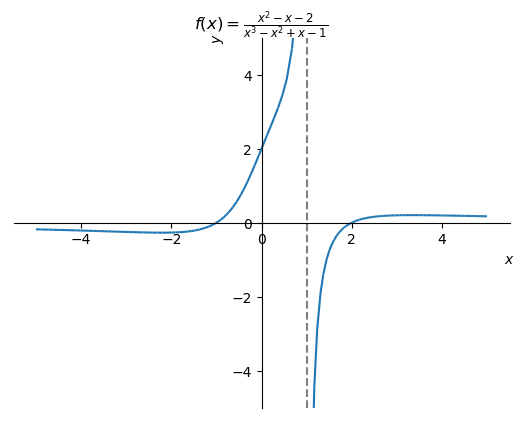
\includegraphics[width=0.8\textwidth]{./cap_funcao/dados/fig_racional_grafico/fig_racional_grafico}
  \caption{Esboço do gráfico da função racional $f(x) = \frac{x^{2} - x - 2}{x^{3} - x^{2} + x - 1}$.}
  \label{fig:racional_grafico}
\end{figure}

Com o estudo do cálculo de limites, veremos que a reta $y = 0$ (eixo das abscissas) é uma assíntota horizontal e a reta $x=1$ (reta tracejada) é uma assíntota vertical ao gráfico desta função. Esta singularidade no ponto $x=1$ está relacionada ao fato de que o denominador se anula em $x=1$. Ainda, para $x\neq 1$ temos
\begin{equation}
  \frac{x^3 - x^2 + x - 1}{x-1} = x^2 + 1,
\end{equation}
Com isso, podemos concluir que o domínio da função $f(x)$ é $\mathbb{R}\setminus\{0\}$.


\subsection*{Exercícios resolvidos}

\begin{flushright}
  [Vídeo] | [Áudio] | \href{https://phkonzen.github.io/notas/contato.html}{[Contatar]}
\end{flushright}

\begin{exer}
  Determine o domínio da função racional
  \begin{equation}
    f(x) = \frac{x^3-x^2+x-1}{x^2-1}.
  \end{equation}
\end{exer}
\begin{resol}
  Como $f(x)$ é uma função racional, ela não está definida nos zeros do polinômio que constitui seu denominador. I.e., nos pontos
  \begin{equation}
    x^2-1=0\Rightarrow x = \pm 1.
  \end{equation}
  Logo, o domínio de $f(x)$ é o conjunto $\mathbb{R}\setminus\{-1, 1\}$.
\end{resol}

\begin{exer}
  Determine o domínio e faça o esboço do gráfico da função racional
  \begin{equation}
    g(x) = \frac{x-1}{x-1}.
  \end{equation}
\end{exer}
\begin{resol}
  Tendo em vista que o denominador se anula em $x=1$, o domínio de $g$ é $(-\infty, 0)\cup (0, \infty)$. Agora, para fazermos um esboço de seu gráfico, observamos que $g(x)=1$ para $x\neq 1$. I.e., $g$ é uma função constante para valores de $x\neq 1$ e não está definida em $x=1$. Veja a Figura \ref{fig:exeresol_funracio_graf} para o esboço do gráfico da função $g$.

  \begin{figure}[H]
    \centering
    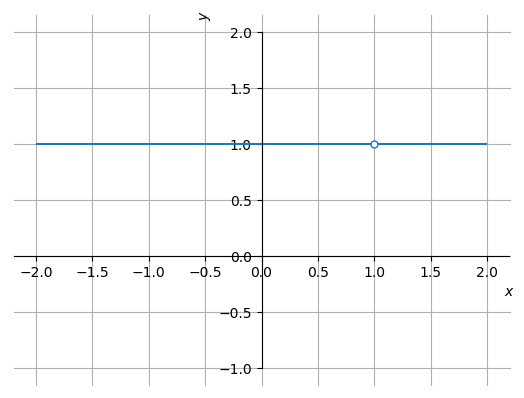
\includegraphics[width=0.8\textwidth]{./cap_funcao/dados/fig_exeresol_funracio_graf/fig_exeresol_funracio_graf}
    \caption{Esboço do gráfico da função $g(x) = (x-1)/(x-1)$.}
    \label{fig:exeresol_funracio_graf}
  \end{figure}

  \ifispython
  Com o \sympy, o comando
\begin{verbatim}
plot((x-1)/(x-1),(x,-2,2))
\end{verbatim}
  plota uma linha constante, sem identificar a singularidade em $x=1$. Isto ocorre, pois os gráficos com o \sympy~ são obtidos a partir de uma amostra discreta de pontos. Ocorre que esta amostra pode não conter as singularidades. No caso de conter, a execução pode não plotar o gráfico e retornar um erro.

  Devemos ficar atentos a esboços de gráficos obtidos no computador, muitas vezes os gráficos podem estar errados. Cabe ao usuário identificar e analisar pontos e região de interesse.
  \fi
\end{resol}

\subsection*{Exercícios}

\begin{flushright}
  [Vídeo] | [Áudio] | \href{https://phkonzen.github.io/notas/contato.html}{[Contatar]}
\end{flushright}

\begin{exer}
  Determine o domínio da função racional
  \begin{equation}
    f(x) = \frac{x^2-1}{x^3-x}.
  \end{equation}
\end{exer}
\begin{resp}
  $\mathbb{R}\setminus\{0\}$
\end{resp}


\section{Funções trigonométricas}\label{cap_funcao_sec_funtri}

\begin{flushright}
  [Vídeo] | [Áudio] | \href{https://phkonzen.github.io/notas/contato.html}{[Contatar]}
\end{flushright}

\subsection{Seno e cosseno}

\begin{flushright}
  [Vídeo] | [Áudio] | \href{https://phkonzen.github.io/notas/contato.html}{[Contatar]}
\end{flushright}

As funções trigonométricas seno $y=\sen(x)$ e cosseno $y=\cos(x)$ podem ser definidas a partir do círculo trigonométrico (veja a Figura \ref{fig:cos_seno}). Seja $x$ o ângulo\footnote{Em geral utilizaremos a medida em radianos para ângulos.} de declividade da reta que passa pela origem do plano cartesiano (reta $r$ na Figura \ref{fig:cos_seno}). Seja, então, $(a,b)$ o ponto de interseção desta reta com a circunferência unitária\footnote{Circunferência do círculo de raio 1.}. Então, definimos:
\begin{equation}
  \sen(x) = a,\qquad \cos(x) = b.
\end{equation}
A partir da definição, notemos que ambas funções têm domínio $(-\infty, \infty)$ e imagem $[-1, 1]$.

\begin{figure}[H]
  \centering
  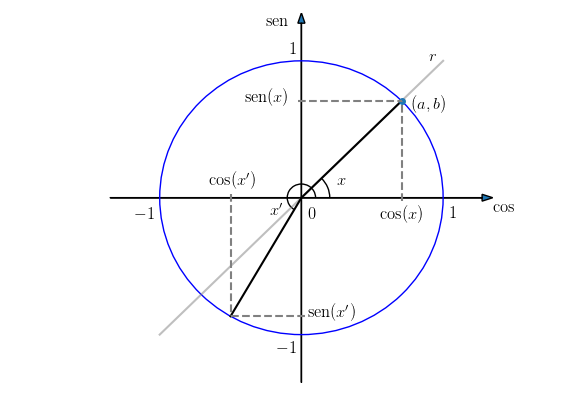
\includegraphics[width=0.8\textwidth]{./cap_funcao/dados/fig_cos_seno/fig_cos_seno}
  \caption{Funções seno e cosseno no círculo trigonométrico.}
  \label{fig:cos_seno}
\end{figure}

Na Figura \ref{fig:cos_seno_valores} podemos extrair os valores das funções seno e cosseno para os ângulos fundamentais. Por exemplo, temos
\begin{align}
  &\sen\left(\frac{\pi}{6}\right) = \frac{1}{2},\qquad \cos\left(\frac{\pi}{6}\right) = \frac{\sqrt{3}}{2},\\
  &\sen\left(\frac{3\pi}{4}\right) = \frac{\sqrt{2}}{2},\qquad \cos\left(\frac{\pi}{4}\right) = -\frac{\sqrt{2}}{2},\\
  &\sen\left(\frac{8\pi}{6}\right) = -\frac{\sqrt{3}}{2},\qquad \cos\left(\frac{8\pi}{6}\right) = -\frac{1}{2},\\
  &\sen\left(\frac{11\pi}{6}\right) = -\frac{1}{2},\qquad \cos\left(\frac{11\pi}{6}\right) = \frac{\sqrt{3}}{2},\\
\end{align}
\ifispython
As funções seno e cosseno estão definidas no \sympy~ como \verb+sin+ e $\verb+cos+$, respectivamente. Por exemplo, para computar o seno de $\pi/6$, digitamos:
\begin{verbatim}
sin(pi/6)
\end{verbatim}
\fi

\begin{figure}[H]
  \centering
  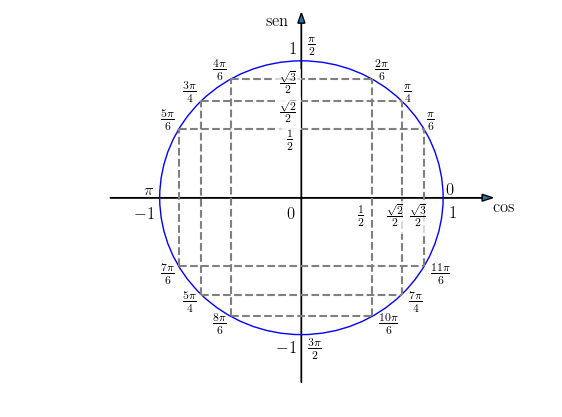
\includegraphics[width=0.8\textwidth]{./cap_funcao/dados/fig_cos_seno_valores/fig_cos_seno_valores}
  \caption{Funções seno e cosseno no círculo trigonométrico.}
  \label{fig:cos_seno_valores}
\end{figure}

Uma \emph{função} $f(x)$ é dita \emph{periódica} quando existe um número $p$, chamado de período da função, tal que
\begin{equation}
  f(x+p) = f(x)
\end{equation}
para qualquer valor de $x$ no domínio da função. Da definição das funções seno e cosseno, notemos que ambas são periódicas com período $2\pi$, i.e.
\begin{equation}
  \sen(x+2\pi) = \sen(x),\qquad \cos(x+2\pi) = \cos(x),
\end{equation}
para qualquer valor de $x$.

Na Figura \ref{fig:cos_seno_graficos}, temos os esboços dos gráficos das funções seno e cosseno.

\begin{figure}[H]
  \centering
  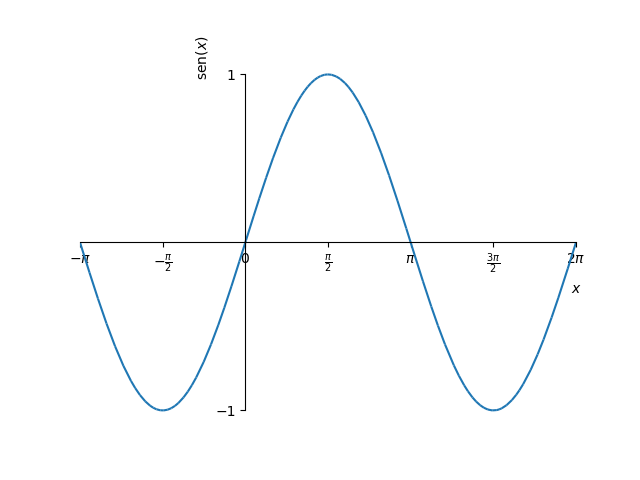
\includegraphics[width=0.5\textwidth]{./cap_funcao/dados/fig_cos_seno_graficos/fig_seno_grafico}~
  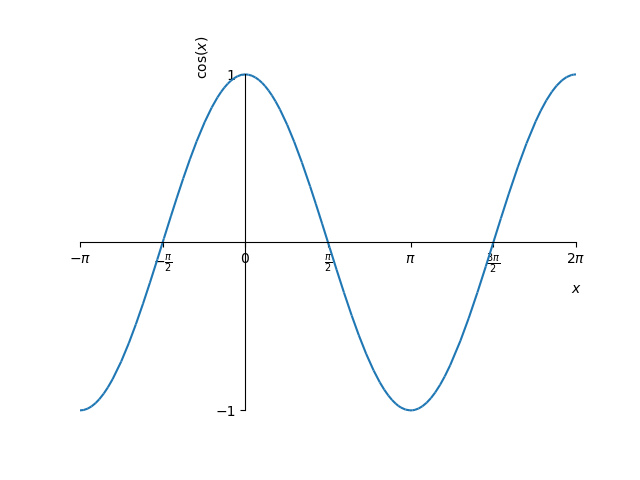
\includegraphics[width=0.5\textwidth]{./cap_funcao/dados/fig_cos_seno_graficos/fig_cosseno_grafico}
  \caption{Esboços dos gráficos das funções seno (esquerda) e cosseno (direita).}
  \label{fig:cos_seno_graficos}
\end{figure}

\subsection{Tangente, cotangente, secante e cossecante}

\begin{flushright}
  [Vídeo] | [Áudio] | \href{https://phkonzen.github.io/notas/contato.html}{[Contatar]}
\end{flushright}

Das funções seno e cosseno, definimos as funções \emph{tangente}, \emph{cotangente}, \emph{secante} e \emph{cossecante} como seguem:
\begin{align}
  \tg(x) := \frac{\sen(x)}{\cos(x)},\qquad \cotg(x) := \frac{\cos(x)}{\sen(x)},\\
  \sec(x) := \frac{1}{\cos(x)},\qquad \cosec(x) := \frac{1}{\sen(x)}.
\end{align}

\ifispython
No \sympy, as funções tangente, cotangente, secante e cossecante podem ser computadas com as funções $\verb+tan+$, $\verb+cot+$, $\verb+sec+$ e $\verb+csc+$, respectivamente. Por exemplo, podemos computar o valor de $\cosec(\pi/4)$ com o comando
\begin{verbatim}
csc(pi/4)
\end{verbatim}
\fi

Na Figura \ref{fig:co_tg_graficos}, temos os esboços dos gráficos das funções tangente e cotangente. Observemos que a função tangente não está definida nos pontos $(2k+1)\pi/2$, para todo $k$ inteiro. Já, a função cotangente não está definida nos pontos $k\pi$, para todo $k$ inteiro. Ambas estas funções têm imagem $(-\infty, \infty)$ e período $\pi$.

\begin{figure}[H]
  \centering
  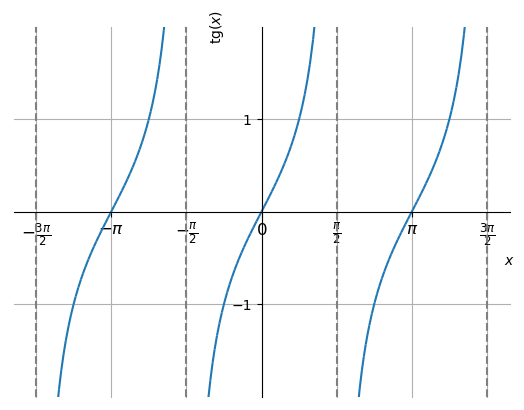
\includegraphics[width=0.5\textwidth]{./cap_funcao/dados/fig_co_tg_graficos/fig_tg_grafico}~
  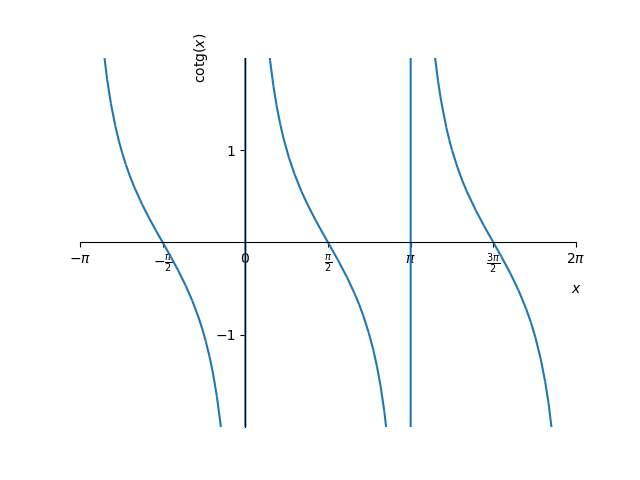
\includegraphics[width=0.5\textwidth]{./cap_funcao/dados/fig_co_tg_graficos/fig_cotg_grafico}
  \caption{Esboços dos gráficos das funções tangente (esquerda) e cotangente(direita).}
  \label{fig:co_tg_graficos}
\end{figure}

Na Figura \ref{fig:co_sec_graficos}, temos os esboços dos gráficos das funções secante e cossecante. Observemos que a função secante não está definida nos pontos $(2k+1)\pi/2$, para todo $k$ inteiro. Já, a função cossecante não está definida nos pontos $k\pi$, para todo $k$ inteiro. Ambas estas funções têm imagem $(-\infty, 1]\cup [1, \infty)$ e período $\pi$.

\begin{figure}[H]
  \centering
  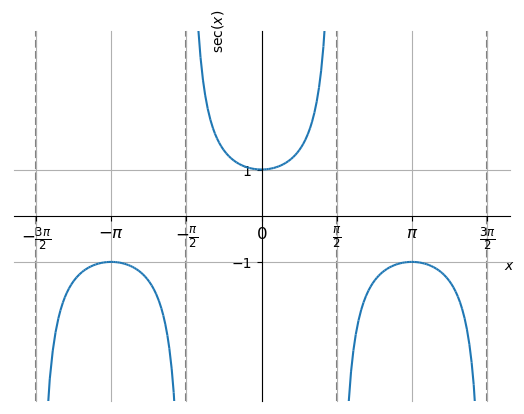
\includegraphics[width=0.5\textwidth]{./cap_funcao/dados/fig_co_sec_graficos/fig_sec_grafico}~
  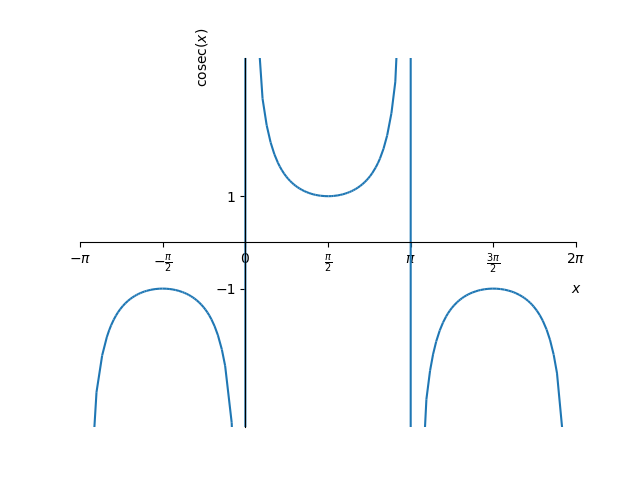
\includegraphics[width=0.5\textwidth]{./cap_funcao/dados/fig_co_sec_graficos/fig_cosec_grafico}
  \caption{Esboços dos gráficos das funções tangente (esquerda) e cotangente(direita).}
  \label{fig:co_sec_graficos}
\end{figure}

\subsection{Identidades trigonométricas}

\begin{flushright}
  [Vídeo] | [Áudio] | \href{https://phkonzen.github.io/notas/contato.html}{[Contatar]}
\end{flushright}

Aqui, vamos apresentar algumas identidades trigonométricas que serão utilizadas ao longo do curso de cálculo. Comecemos pela identidade fundamental
\begin{equation}
  \sen^2 x + \cos^2 x = 1.
\end{equation}
Desta decorrem as identidades
\begin{align}
  &\tg^2(x) + 1 = \sec^2 x,\\
  &1 + \cotg^2(x) = \cosec^2(x).
\end{align}

Das seguintes fórmulas para adição/subtração de ângulos
\begin{align}
  &\cos(x\pm y) = \cos(x)\cos(y) \mp \sen(x)\sen(y),\\
  &\sen(x\pm y) = \sen(x)cos(y) \pm \cos(x)\sen(y),
\end{align}
seguem as fórmulas para ângulo duplo
\begin{align}
  &\cos(2x) = \cos^2x - \sen^2x,\\
  &\sen(2x) = 2\sen x\cos x.
\end{align}

Também, temos as fórmulas para o ângulo metade
\begin{align}
  &\cos^2 x = \frac{1 + \cos 2x}{2},\\
  &\sen^2 x = \frac{1 - \cos 2x}{2}.\label{eq:id_trig_cos_x2}
\end{align}

\subsection*{Exercícios resolvidos}

\begin{flushright}
  [Vídeo] | [Áudio] | \href{https://phkonzen.github.io/notas/contato.html}{[Contatar]}
\end{flushright}

\begin{exeresol}
  Mostre que
  \begin{equation}
    \cos x - 1 = -2\sen^2 \frac{x}{2}.
  \end{equation}
\end{exeresol}
\begin{resol}
  A identidade trigonométrica
  \begin{equation}
    \sen^2 x = \frac{1 - \cos 2x}{2},
  \end{equation}
  aplicada a metade do ângulo, fornece
  \begin{equation}
    \sen^2 \frac{x}{2} = \frac{1 - \cos x}{2}.
  \end{equation}
  Então, isolando $\cos x$, obtemos
  \begin{align}
    \sen^2 \frac{x}{2} = \frac{1 - \cos x}{2} &\Rightarrow 1 - \cos x = 2\sen^2 \frac{x}{2}\\
                                              &\Rightarrow \cos x - 1 = -2\sen^2 \frac{x}{2}.
  \end{align}
\end{resol}

\subsection*{Exercícios}

\begin{flushright}
  [Vídeo] | [Áudio] | \href{https://phkonzen.github.io/notas/contato.html}{[Contatar]}
\end{flushright}

\begin{exer}
  Mostre que $\sen x$ é  uma função ímpar, i.e.
  \begin{equation}
    \sen x = \sen(-x)
  \end{equation}
  para todo número real $x$.
\end{exer}
\begin{resp}
  Dica: analise o ciclo trigonométrico.
\end{resp}

\begin{exer}
  Mostre que $\cos x$ é  uma função par, i.e.
  \begin{equation}
    \cos x = -\cos(-x)
  \end{equation}
  para todo número real $x$.
\end{exer}
\begin{resp}
  Dica: analise o ciclo trigonométrico.
\end{resp}

\section{Operações com funções}\label{cap_funcao_sec_opfun}

\begin{flushright}
  [Vídeo] | [Áudio] | \href{https://phkonzen.github.io/notas/contato.html}{[Contatar]}
\end{flushright}

\subsection{Somas, diferenças, produtos e quocientes}

\begin{flushright}
  [Vídeo] | [Áudio] | \href{https://phkonzen.github.io/notas/contato.html}{[Contatar]}
\end{flushright}

Sejam dadas as funções $f$ e $g$ com domínio em comum $D$. Então, definimos as funções
\begin{itemize}
\item $(f\pm g)(x) := f(x) \pm g(x)$ para todo $x\in D$;
\item $(fg)(x) := f(x)g(x)$ para todo $x\in D$;
\item $\displaystyle \left(\frac{f}{g}\right)(x) := \frac{f(x)}{g(x)}$ para todo $x\in D$ tal que $g(x)\neq 0$.
\end{itemize}

\begin{ex}
  Sejam $f(x)=x^2$ e $g(x)=x$. Temos:
  \begin{itemize}
  \item $(f+g)(x) = x^2 + x$ e está definida em toda parte.
  \item $(g-f)(x) = x - x^2$ e está definida em toda parte.
  \item $(fg)(x) = x^3$ e está definida em toda parte.
  \item $\left(\frac{f}{g}\right)(x) = \frac{x^2}{x}$ e tem domínio $(-\infty, \infty)\setminus \{0\}$\footnote{Observemos que não podemos simplificar o $x$, pois a função $y=x$ é diferente da função $y=x^2/x$.}.
  \end{itemize}
\end{ex}

\subsection{Funções compostas}

\begin{flushright}
  [Vídeo] | [Áudio] | \href{https://phkonzen.github.io/notas/contato.html}{[Contatar]}
\end{flushright}

Sejam dadas as funções $f$ e $g$. Definimos a \emph{função composta} de $f$ com $g$ por
\begin{equation}
  (f\circ g)(x) := f(g(x)).
\end{equation}
Seu domínio consiste dos valores de $x$ que pertençam ao domínio da $g$ e tal que $g(x)$ pertença ao domínio da $f$.

\begin{ex}
  Sejam $f(x) = x^2$ e $g(x) = x+1$. A função composta $(f\circ g)(x) = f(g(x)) = f(x+1) = (x+1)^2$.
\end{ex}

\subsection{Translações, contrações, dilatações e reflexões de gráficos}

\begin{flushright}
  [Vídeo] | [Áudio] | \href{https://phkonzen.github.io/notas/contato.html}{[Contatar]}
\end{flushright}

Algumas operações com funções produzem resultados bastante característico no gráfico de funções. Com isso, podemos usar estas operações para construir gráficos de funções mais complicadas a partir de funções básicas.

\subsection{Translações}

\begin{flushright}
  [Vídeo] | [Áudio] | \href{https://phkonzen.github.io/notas/contato.html}{[Contatar]}
\end{flushright}

Dada uma função $f$ e uma constante $k\neq 0$, temos que a o gráfico de $y = f(x) + k$ é uma translação vertical do gráfico de $f$. Se $k>0$, observamos uma translação vertical para cima. Se $k<0$, observamos uma translação vertical para baixo.

\begin{ex}
  Seja $f(x) = x^2$. A Figura \ref{fig:ex_trans_vert}, contém os esboços dos gráficos de $f(x)$ e $f(x)+k = x^2+k$ para $k=1$.

  \begin{figure}[H]
    \centering
    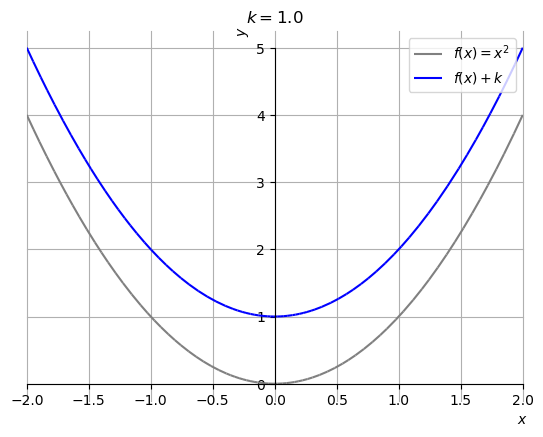
\includegraphics[width=0.7\textwidth]{./cap_funcao/dados/fig_ex_transvert/fig_ex_transvert}
    \caption{Esboço do gráfico de $f(x) = x^2$ e $f(x)+k$ com $k=1$.}
    \label{fig:ex_trans_vert}
  \end{figure}

  \ifispython
  O seguinte código \verb+Python+, faz os esboços dos gráficos de $f(x)$ e $f(x)+k$:
\begin{verbatim}
k = 1
f = lambda x: x**2

p = plot(f(x),(x,-2,2),line_color="gray",show=False)
q = plot(f(x)+k,(x,-2,2),line_color="blue",show=False)
p.extend(q)
p.title = ("$k = %1.1f$" % k)
p.xlabel = '$x$'
p.ylabel = '$y$'
p[0].label = "$f(x) = x^2$"
p[1].label = "$f(x)+k$"
p.save('fig.png')

fig = p._backend.fig
ax = fig.axes[0]
ax.grid()
ax.legend(loc="upper right")
fig.savefig('fig.png', bbox_inches='tight')
\end{verbatim}
  Podemos alterar o valor de $k$ e a função $f$ para vermos o efeito das translações verticais.
  \fi
\end{ex}

Translações horizontais de gráficos podem ser produzidas pela soma de uma constante não nula ao argumento da função. Mais precisamente, dada uma função $f$ e uma constante $k\neq 0$, temos que o gráfico de $y=f(x+k)$ é uma translação horizontal do gráfico de $f$ em $k$ unidades. Se $k>0$, observamos uma translação horizontal para a esquerda. Se $k<0$, observamos uma translação horizontal para a direita.

\begin{ex}
  Seja $f(x) = x^2$. A Figura \ref{fig:ex_transhoriz}, contém os esboços dos gráficos de $f(x)$ e $f(x+k) = (x+k)^2$ para $k=1$.

  \begin{figure}[H]
    \centering
    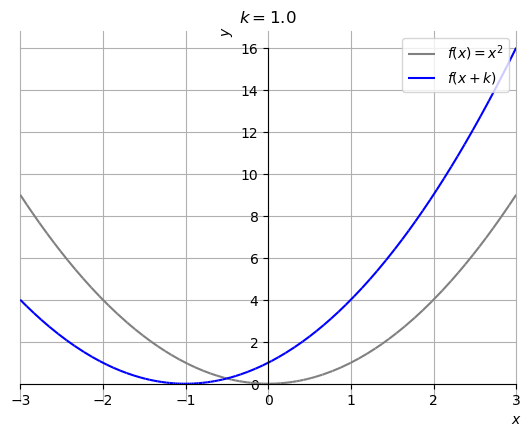
\includegraphics[width=0.7\textwidth]{./cap_funcao/dados/fig_ex_transhoriz/fig_ex_transhoriz}
    \caption{Esboço do gráfico de $f(x) = x^2$ e $f(x+k)$ com $k=1$.}
    \label{fig:ex_transhoriz}
  \end{figure}

  \ifispython
  O seguinte código \verb+Python+, faz os esboços dos gráficos de $f(x)$ e $f(x+k)$:
\begin{verbatim}
k = 1
f = lambda x: x**2

p = plot(f(x),(x,-3,3),line_color="gray",show=False)
q = plot(f(x+k),(x,-3,3),line_color="blue",show=False)
p.extend(q)
p.title = ("$k = %1.1f$" % k)
p.xlabel = '$x$'
p.ylabel = '$y$'
p[0].label = "$f(x) = x^2$"
p[1].label = "$f(x+k)$"
p.save('fig.png')

fig = p._backend.fig
ax = fig.axes[0]
ax.grid()
ax.legend(loc="upper right")
fig.savefig('fig.png', bbox_inches='tight')
\end{verbatim}
  Podemos alterar o valor de $k$ e a função $f$ para vermos o efeito das translações horizontais.
  \fi
\end{ex}

\subsection{Dilatações e contrações}

\begin{flushright}
  [Vídeo] | [Áudio] | \href{https://phkonzen.github.io/notas/contato.html}{[Contatar]}
\end{flushright}

Sejam dados uma função $f$ e uma constante $\alpha$. Então, o gráfico de:
\begin{itemize}
\item $y = \alpha f(x)$ é uma dilatação vertical do gráfico de $f$, quando $\alpha > 1$;
\item $y = \alpha f(x)$ é uma contração vertical do gráfico de $f$, quando $0<\alpha < 1$;
\item $y = f(\alpha x)$ é uma contração horizontal do gráfico de $f$, quando $\alpha > 1$;
\item $y = f(\alpha x)$ é uma dilatação horizontal do gráfico de $f$, quando $0<\alpha < 1$.
\end{itemize}

\begin{ex}
  Seja $f(x) = x^2$. A Figura \ref{fig:ex_dilavert}, contém os esboços dos gráficos de $f(x)$ e $\alpha\cdot f(x) = \alpha \cdot x^2$ para $\alpha = 2$.

  \begin{figure}[H]
    \centering
    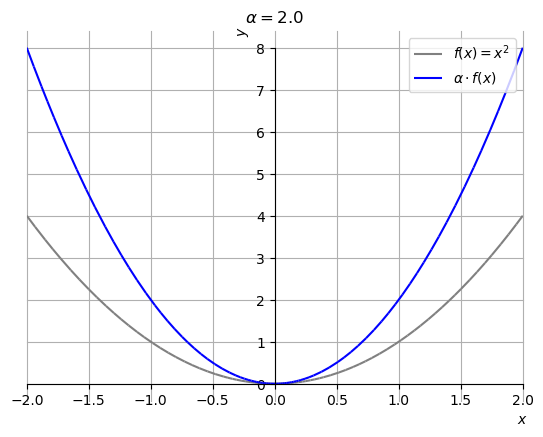
\includegraphics[width=0.7\textwidth]{./cap_funcao/dados/fig_ex_dilavert/fig_ex_dilavert}
    \caption{Esboço do gráfico de $f(x) = x^2$ e $\alpha\cdot f(x)$ com $\alpha=2$.}
    \label{fig:ex_dilavert}
  \end{figure}

  \ifispython
  O seguinte código \verb+Python+, faz os esboços dos gráficos de $f(x)$ e $\alpha\cdot f(x)$:
\begin{verbatim}
alpha = 2
f = lambda x: x**2

p = plot(f(x),(x,-2,2),line_color="gray",show=False)
q = plot(alpha*f(x),(x,-2,2),line_color="blue",show=False)
p.extend(q)
p.title = ("$\\alpha = %1.1f$" % alpha)
p.xlabel = '$x$'
p.ylabel = '$y$'
p[0].label = "$f(x) = x^2$"
p[1].label = "$\\alpha\\cdot f(x)$"
p.save('fig_ex_dilavert.png')

fig = p._backend.fig
ax = fig.axes[0]
ax.grid()
ax.legend(loc="upper right")
fig.savefig('fig_ex_dilavert.png', bbox_inches='tight')
\end{verbatim}
  Podemos alterar o valor de \verb+alpha+ e a função \verb+f+ para vermos o efeito das dilatações/contrações verticais.
  \fi
\end{ex}

\begin{ex}
  Seja $f(x) = x^2-2x+1$. A Figura \ref{fig:ex_dilahoriz}, contém os esboços dos gráficos de $f(x)$ e $f(\alpha\cdot x) = (\alpha \cdot x)^2-2(\alpha\cdot x) + 1$ para $\alpha = \frac{1}{2}$.

  \begin{figure}[H]
    \centering
    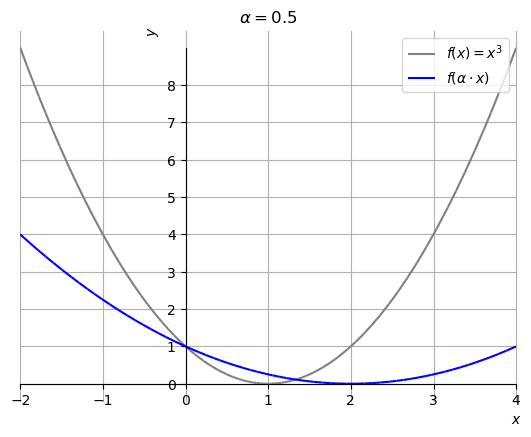
\includegraphics[width=0.7\textwidth]{./cap_funcao/dados/fig_ex_dilahoriz/fig_ex_dilahoriz}
    \caption{Esboço do gráfico de $f(x) = x^2-2x+1$ e $f(\alpha\cdot x)$ com $\alpha=\frac{1}{2}$.}
    \label{fig:ex_dilahoriz}
  \end{figure}

  \ifispython
  O seguinte código \verb+Python+, faz os esboços dos gráficos de $f(x)$ e $f(\alpha\cdot x)$:
\begin{verbatim}
alpha = 0.5
f = lambda x: x**2-2*x+1

p = plot(f(x),(x,-2,4),line_color="gray",show=False)
q = plot(f(alpha*x),(x,-2,4),line_color="blue",show=False)
p.extend(q)
p.title = ("$\\alpha = %1.1f$" % alpha)
p.xlabel = '$x$'
p.ylabel = '$y$'
p[0].label = "$f(x) = x^3$"
p[1].label = "$f(\\alpha\\cdot x)$"
p.save('fig_ex_dilahoriz.png')

fig = p._backend.fig
ax = fig.axes[0]
ax.grid()
ax.set_yticks(range(0,9))
ax.legend(loc="upper right")
fig.savefig('fig_ex_dilahoriz.png', bbox_inches='tight')
\end{verbatim}
  Podemos alterar o valor de \verb+alpha+ e a função \verb+f+ para vermos o efeito das dilatações/contrações horizontais.
  \fi
\end{ex}


\subsection{Reflexões}

\begin{flushright}
  [Vídeo] | [Áudio] | \href{https://phkonzen.github.io/notas/contato.html}{[Contatar]}
\end{flushright}

Seja dada uma função $f$. O gráfico da função $y = -f(x)$ é uma reflexão em torno do eixo das abscissas do gráfico da função $f$. Já, o gráfico da função $y = f(-x)$ é uma reflexão em torno do eixo das ordenadas do gráfico da função $f$.

\begin{ex}
  Seja $f(x) = x^2-2x+2$. A Figura \ref{fig:ex_reflex}, contém os esboços dos gráficos de $f(x)$ e $-f(x) = -x^2+2x-2$.

  \begin{figure}[H]
    \centering
    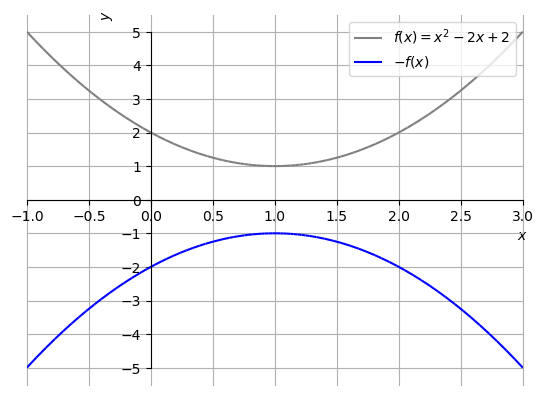
\includegraphics[width=0.7\textwidth]{./cap_funcao/dados/fig_ex_reflex/fig_ex_reflex}
    \caption{Esboço do gráfico de $f(x) = x^2-2x+2$ e $-f(x)$.}
    \label{fig:ex_reflex}
  \end{figure}

  \ifispython
  O seguinte código \verb+Python+, faz os esboços dos gráficos de $f(x)$ e $-f(x)$:
\begin{verbatim}
f = lambda x: x**2-2*x+2

p = plot(f(x),(x,-1,3),line_color="gray",show=False)
q = plot(-f(x),(x,-1,3),line_color="blue",show=False)
p.extend(q)
p.xlabel = '$x$'
p.ylabel = '$y$'
p[0].label = "$f(x) = x^2-2x+2$"
p[1].label = "$-f(x)$"
p.save('fig_ex_reflex.png')

fig = p._backend.fig
ax = fig.axes[0]
ax.grid()
ax.set_yticks(range(-5,6))
ax.legend(loc="upper right")
fig.savefig('fig_ex_reflex.png', bbox_inches='tight')
\end{verbatim}
  Podemos alterar a função \verb+f+ para vermos o efeito das reflexões em torno de eixo das abscissas.
  \fi
\end{ex}


\begin{ex}
  Seja $f(x) = x^2-2x+2$. A Figura \ref{fig:ex_refley}, contém os esboços dos gráficos de $f(x)$ e $f(-x) = x^2+2x+2$.

  \begin{figure}[H]
    \centering
    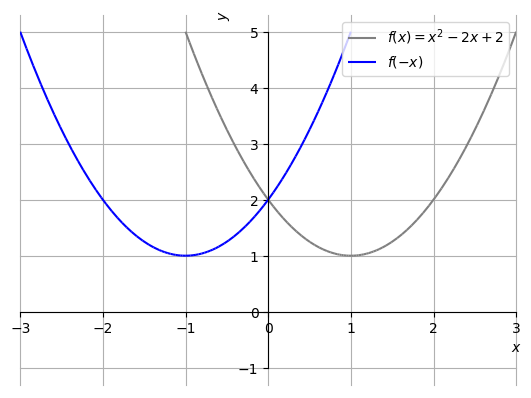
\includegraphics[width=0.7\textwidth]{./cap_funcao/dados/fig_ex_refley/fig_ex_refley}
    \caption{Esboço do gráfico de $f(x) = x^2-2x+2$ e $f(-x)$.}
    \label{fig:ex_reflex}
  \end{figure}

  \ifispython
  O seguinte código \verb+Python+, faz os esboços dos gráficos de $f(x)$ e $f(-x)$:
\begin{verbatim}
f = lambda x: x**2-2*x+2

p = plot(f(x),(x,-1,3),line_color="gray",show=False)
q = plot(f(-x),(x,-3,1),line_color="blue",show=False)
p.extend(q)
q = plot(-1,(x,-3,3),line_color="none",show=False)
p.extend(q)
p.xlabel = '$x$'
p.ylabel = '$y$'
p[0].label = "$f(x) = x^2-2x+2$"
p[1].label = "$f(-x)$"
p[2].label = ""
p.save('fig_ex_refley.png')

fig = p._backend.fig
ax = fig.axes[0]
ax.grid()
ax.set_yticks(range(-1,6))
ax.legend(loc="upper right")
fig.savefig('fig_ex_refley.png', bbox_inches='tight')
\end{verbatim}
  Podemos alterar a função \verb+f+ para vermos o efeito das reflexões em torno de eixo das ordenadas.
  \fi
\end{ex}

\subsection*{Exercícios resolvidos}

\begin{flushright}
  [Vídeo] | [Áudio] | \href{https://phkonzen.github.io/notas/contato.html}{[Contatar]}
\end{flushright}

\begin{exeresol}
  Sejam
  \begin{equation}
    f(x) = \frac{x^2 - \sqrt{x-1}}{x}\quad\text{e}\quad g(x) = x^2 + 1.
  \end{equation}
  Determine a função composta $(f\circ g)$ e seu domínio.
\end{exeresol}
\begin{resol}
  Começamos determinando a função composta
  \begin{align}
    (f\circ g)(x) &:= f(g(x))\\
                  &= f(x^2 + 1)\\
                  &= \frac{(x^2 + 1)^2 - \sqrt{x^2+1-1}}{x^2 + 1}\\
                  &= \frac{x^4 + 2x^2 + 1 - \sqrt{x^2}}{x^2 + 1}\\
                  &= \frac{x^4 + 2x^2 + 1 - |x|}{x^2 + 1}.
  \end{align}
  Agora, observamos que $g$ está definida em toda parte e tem imagem $[1, \infty)$. Como o domínio da $f$ é $[1, \infty)$, temos que $(f\circ g)$ está definida em toda parte.
\end{resol}

\begin{exeresol}
  Faça o esboço do gráfico de $f(x) = 2(x-1)^3+1$.
\end{exeresol}
\begin{resol}
  Começamos trançando o gráfico de $f_1(x) = x^3$. Então, obtemos o gráfico de $f_2(x) = (x-1)^3$ por translação de uma unidade à direita. O gráfico de $f_3(x) = 2(x-1)^3$ é obtido por dilatação vertical de 2 vezes. Por fim, o gráfico de $f_4(x) = 2(x-1)^3+1$ é obtido por translação de uma unidade para cima. Veja a Figura \ref{fig:exeresol_opfun_graf}.

  \begin{figure}[H]
    \centering
    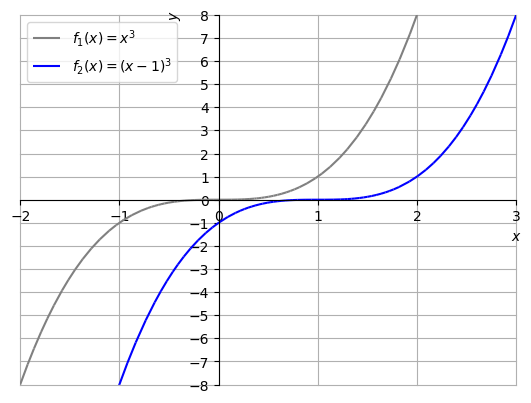
\includegraphics[width=0.49\textwidth]{./cap_funcao/dados/fig_exeresol_opfun_graf/fig_exeresol_opfun_graf_1}~
    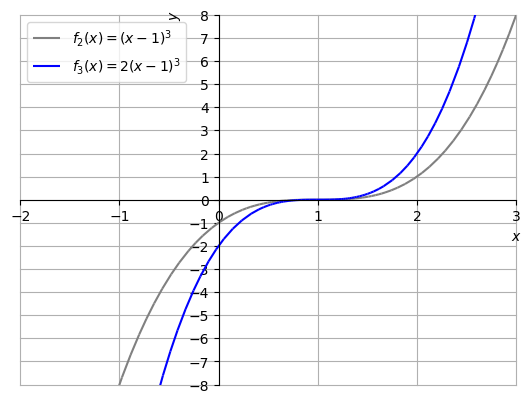
\includegraphics[width=0.49\textwidth]{./cap_funcao/dados/fig_exeresol_opfun_graf/fig_exeresol_opfun_graf_2}\\
    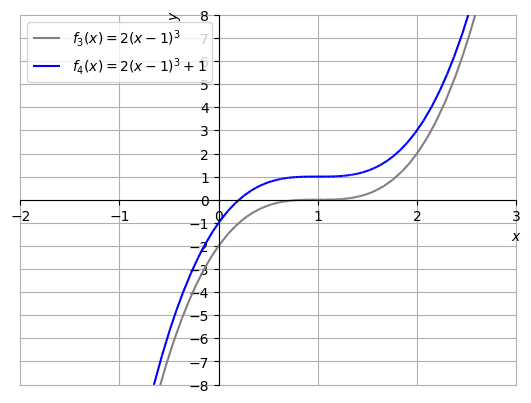
\includegraphics[width=0.49\textwidth]{./cap_funcao/dados/fig_exeresol_opfun_graf/fig_exeresol_opfun_graf_3}
    \caption{Construção do esboço do gráfico de $f(x) = 2(x-1)^3+1$.}
    \label{fig:exeresol_opfun_graf}
  \end{figure}
\end{resol}

\subsection*{Exercícios}

\begin{flushright}
  [Vídeo] | [Áudio] | \href{https://phkonzen.github.io/notas/contato.html}{[Contatar]}
\end{flushright}

\begin{exer}
  Sejam $f(x) = \sqrt{x}+1$ e $g(x) = x^2 -1$. Determine a função $(f\circ g)$ e seu domínio.
\end{exer}
\begin{resp}
  $(f\circ g)(x) = \sqrt{x^2-1}+1$; domínio: $(-\infty, 1]\cup [1, \infty)$.
\end{resp}

\begin{exer}
  Faça um esboço do gráfico de $g(x) = 2x^3 - 1$.
\end{exer}
\begin{resp}
  Dica: verifique sua resposta com um pacote de matemática simbólica, por exemplo, com o \sympy.
\end{resp}

\section{Propriedades de funções}\label{cap_funcao_sec_funprop}

\begin{flushright}
  [Vídeo] | [Áudio] | \href{https://phkonzen.github.io/notas/contato.html}{[Contatar]}
\end{flushright}

\subsection{Funções crescentes ou decrescentes}

\begin{flushright}
  [Vídeo] | [Áudio] | \href{https://phkonzen.github.io/notas/contato.html}{[Contatar]}
\end{flushright}

Uma da função $f$ é dita ser crescente quando $f(x_1)<f(x_2)$ para todos $x_1<x_2$ no seu domínio. É dita não decrescente quando $f(x_1)\leq f(x_2)$ para todos os $x_1<x_2$ no seu domínio. Analogamente, é dita decrescente quando $f(x_1)>f(x_2)$ para todos $x_1<x_2$. E, por fim, é dita não crescente quando $f(x_1)\geq f(x_2)$ para todos $x_1<x_2$, sempre no seu domínio.

\begin{ex}
  Vejamos os seguintes casos:
  \begin{itemize}
  \item A \emph{função identidade} $f(x)=x$ é crescente.
  \item A seguinte função definida por partes
    \begin{equation}
      f(x) = \left\{
        \begin{array}{ll}
          x+1 &,x\leq 0,\\
          2 &,0<x\leq 1,\\
          (x-1)^2+2 &, x>1
        \end{array}
\right.
\end{equation}
é não decrescente.
  \end{itemize}
\end{ex}

Também, definem-se os conceitos análogos de uma função ser crescente ou decrescente em um dado intervalo.

\begin{ex}
  A função $f(x) = x^2$ é uma função decrescente no intervalo $(-\infty, 0]$ e crescente no intervalo $[0, \infty)$.
\end{ex}

\subsection{Funções pares ou ímpares}

\begin{flushright}
  [Vídeo] | [Áudio] | \href{https://phkonzen.github.io/notas/contato.html}{[Contatar]}
\end{flushright}

Uma dada \emph{função} $f$ é dita \emph{par} quando $f(x)=f(-x)$ para todo $x$ no seu domínio. Ainda, é dita \emph{ímpar} quando $f(x)=-f(-x)$ para todo $x$ no seu domínio.

\begin{ex}
  Vejamos os seguintes casos:
  \begin{itemize}
  \item $f(x) = x^2$ é uma função par.
  \item $f(x) = x^3$ é uma função par.
  \item $f(x) = \sen x$ é uma função ímpar.
  \item $f(x) = \cos x$ é uma função par.
  \item $f(x) = x+1$ não é par nem ímpar.
  \end{itemize}
\end{ex}

\subsection{Funções injetoras}

\begin{flushright}
  [Vídeo] | [Áudio] | \href{https://phkonzen.github.io/notas/contato.html}{[Contatar]}
\end{flushright}

Uma dada {\bf função} $f$ é dita {\bf injetora} quando $f(x_1)\neq f(x_2)$ para todos $x_1\neq x_2$ no seu domínio.

\begin{ex}
  Vejamos os seguintes casos:
  \begin{itemize}
  \item $f(x) = x^2$ não é uma função injetora.
  \item $f(x) = x^3$ é uma função injetora.
  \item $f(x) = e^x$ é uma função injetora.
  \end{itemize}
\end{ex}

Função injetoras são funções invertíveis. Mais precisamente, dada uma função injetora $y = f(x)$, existe uma única função $g$ tal que
\begin{equation}
  g(f(x)) = x,
\end{equation}
para todo $x$ no domínio da $f$. Tal função $g$ é chamada de \emph{função inversa} de $f$ é comumente denotada por $f^{-1}$.\footnote{Observe que, em geral, $f^{-1} \neq \frac{1}{f}$.}

\begin{ex}
  Vamos calcular a função a função inversa de $f(x) = x^3 + 1$. Para tando, escrevemos
  \begin{equation}
    y = x^3 + 1.
  \end{equation}
  Então, isolando $x$, temos
  \begin{equation}
    x = \sqrt[3]{y - 1}.
  \end{equation}
  Desta forma, concluímos que $f^{-1}(x) = \sqrt[3]{x-1}$. Verifique que $f^{-1}(f(x)) = x$ para todo $x$ no domínio de $f$!
\end{ex}

\begin{obs}
 Os gráficos de uma dada função injetora $f$ e de sua inversa $f^{-1}$ são simétricos em relação a \emph{reta identidade} $y=x$.
\end{obs}

\subsection*{Exercícios resolvidos}

\begin{flushright}
  [Vídeo] | [Áudio] | \href{https://phkonzen.github.io/notas/contato.html}{[Contatar]}
\end{flushright}

\begin{exeresol}
  Defina os intervalos em que a função $f(x) = -|x+1|$ é crescente ou decrescente.
\end{exeresol}
\begin{resol}
  A função $f$ é uma translação à esquerda, seguida de uma reflexão em torno do eixo das abscissas da função $f(x) = |x|$. Veja a Figura \ref{fig:exeresol_funprop_mono}.

  \begin{figure}[H]
    \centering
    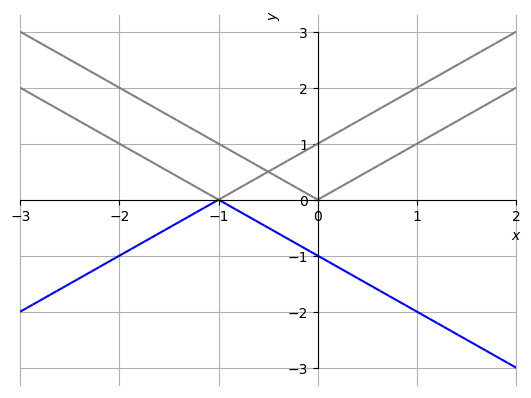
\includegraphics[width=0.6\textwidth]{./cap_funcao/dados/fig_exeresol_funprop_mono/fig_exeresol_funprop_mono.png}
    \caption{Esboço do gráfico de $f(x) = -|x+1|$.}
    \label{fig:exeresol_funprop_mono}
  \end{figure}

  Do esboço do gráfico de $f$, podemos inferir que $f$ é crescente no intervalo $(-\infty, -1]$ e decrescente no intervalo $[-1, \infty)$.
\end{resol}

\begin{exeresol}
  Analise a paridade da função $tg(x)$.
\end{exeresol}
\begin{resol}
  Da paridade das funções seno e cosseno, temos
  \begin{equation}
    \tg(-x) = \frac{\sen(-x)}{\cos(-x)} = \frac{-\sen x}{\cos x} = -\frac{\sen x}{\cos x} = -\tg x.
  \end{equation}
  Logo, a tangente é uma função ímpar.
\end{resol}

\begin{exeresol}
  Calcule a função inversa de $f(x) = \sqrt{x+1}$.
\end{exeresol}
\begin{resol}
  Para obtermos a função inversa de uma função $f$, resolvemos $y = f(x)$ para $x$. Ou seja,
  \begin{align}
    y = f(x) &\Rightarrow y = \sqrt{x+1}\\
             &\Rightarrow y^2 = x+1\\
             &\Rightarrow x = y^2 - 1.
  \end{align}
  Logo, temos $f^{-1}(x) = x^2 - 1$ restrita ao conjunto imagem da $f$, i.e. o domínio de $f^{-1}$ é $[0, \infty)$.
\end{resol}

\subsection*{Exercícios}

\begin{flushright}
  [Vídeo] | [Áudio] | \href{https://phkonzen.github.io/notas/contato.html}{[Contatar]}
\end{flushright}

\begin{exer}
  Determine os intervalos de crescimento ou decrescimento da função
  \begin{equation}
    f(x) = \left\{
      \begin{array}{ll}
        (x+1)^2 &, -\infty < x \leq 1,\\
        -x+5 &, 1 \leq x < \infty
      \end{array}
\right.
  \end{equation}
\end{exer}
\begin{resp}
  decrescente: $(-\infty, -1]\cup [1, \infty)$; crescente: $[-1, 1]$.
\end{resp}

\begin{exer}
  Analise a paridade da função $\cosec x$.
\end{exer}
\begin{resp}
  função ímpar
\end{resp}

\begin{exer}
  Seja $f(x) = 2\sqrt{x-1}-1$. Calcule $f^{-1}$ e determine seu domínio.
\end{exer}
\begin{resp}
  $f^{-1}(x) = \frac{1}{2}x^2 + x - \frac{1}{2}$; domínio $[-1, \infty)$
\end{resp}

\section{Funções exponenciais}\label{cap_funcao_sec_funexp}

\begin{flushright}
  [Vídeo] | [Áudio] | \href{https://phkonzen.github.io/notas/contato.html}{[Contatar]}
\end{flushright}

Uma \emph{função exponencial} tem a forma
\begin{equation}
  f(x) = a^x,
\end{equation}
onde $a\neq 1$ é uma constante positiva e é chamada de \emph{base} da função exponencial.

Funções exponenciais estão definidas em toda parte e têm imagem $(0, \infty)$. O gráfico de uma função exponencial sempre contém os pontos $(-1,1/a)$, $(0,1)$ e $(1,a)$. Veja a Figura \ref{fig:exponencial_graficos}.

\begin{figure}[H]
  \centering
  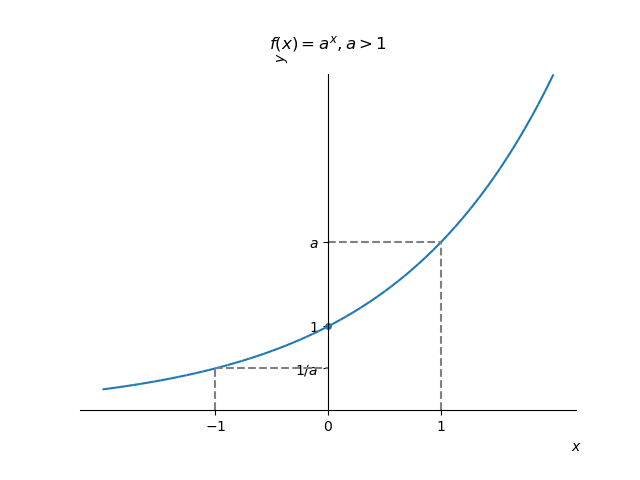
\includegraphics[width=0.5\textwidth]{./cap_funcao/dados/fig_exponencial_graficos/fig_exponencial_2}~
  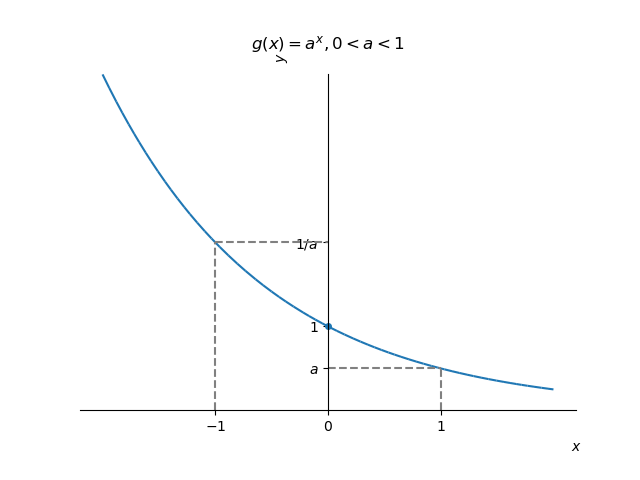
\includegraphics[width=0.5\textwidth]{./cap_funcao/dados/fig_exponencial_graficos/fig_exponencial_12}
  \caption{Esboços dos gráficos de funções exponenciais: (esquerda) $f(x) = a^x$, $a>1$; (direita) $g(x) = a^x$, $0<a<1$.}
  \label{fig:exponencial_graficos}
\end{figure}

\begin{obs}
  Quando a base é o número de Euler $e \approx 2,718281828459045$, chamamos $f(x) = e^x$ de função exponencial natural.

  \ifispython
  No \sympy\footnote{Veja a Observação \ref{obs:cap_funcao_python}}, o número de Euler é obtido com a constante \verb+E+:
\begin{verbatim}
>>> float(E)
2.718281828459045
\end{verbatim}
  \fi
\end{obs}

\subsection*{Exercícios resolvidos}

\begin{flushright}
  [Vídeo] | [Áudio] | \href{https://phkonzen.github.io/notas/contato.html}{[Contatar]}
\end{flushright}

\begin{exeresol}
  Faça um esboço do gráfico de $f(x) = e^{-2x+1}-1$.
\end{exeresol}
\begin{resol}
  Primeiramente, observamos que $f(x) = e^{-2x+1}-1 = e^{-2\left(x-\frac{1}{2}\right)}-1$. Então, partindo do gráfico de $e^{-x}$, fazemos uma translação de $\frac{1}{2}$ unidades à direita, seguida de uma contração horizontal de $\frac{1}{2}$ vezes e, por fim, uma translação para baixo de uma unidade. Veja a Figura \ref{fig:exeresol_funexp_graf}.

  \begin{figure}[H]
    \centering
    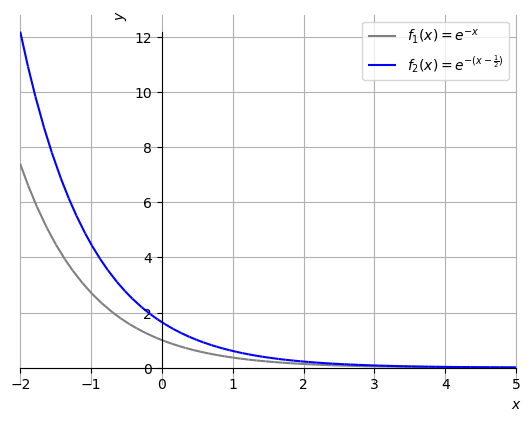
\includegraphics[width=0.49\textwidth]{./cap_funcao/dados/fig_exeresol_funexp_graf/fig_exeresol_funexp_graf_1}~
    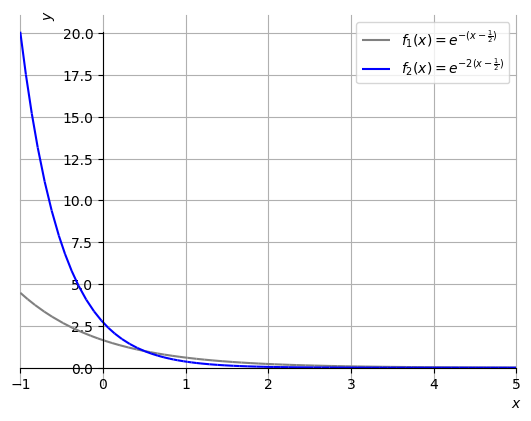
\includegraphics[width=0.49\textwidth]{./cap_funcao/dados/fig_exeresol_funexp_graf/fig_exeresol_funexp_graf_2}\\
    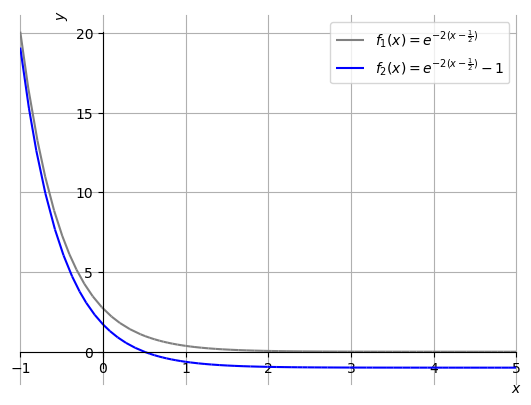
\includegraphics[width=0.49\textwidth]{./cap_funcao/dados/fig_exeresol_funexp_graf/fig_exeresol_funexp_graf_3}
    \caption{Esboço do gráfico de $f(x) = e^{-2x+1}-1$.}
    \label{fig:exeresol_funexp_graf}
  \end{figure}
\end{resol}

\subsection*{Exercícios}

\begin{flushright}
  [Vídeo] | [Áudio] | \href{https://phkonzen.github.io/notas/contato.html}{[Contatar]}
\end{flushright}

\begin{exer}
  Faça um esboço do gráfico de $f(x) = 2e^{x-1}+2$.
\end{exer}
\begin{resp}
  Dica: use um pacote de matemática simbólica para verificar sua resposta.
\end{resp}

\section{Funções logarítmicas}\label{cap_funcao_sec_funlog}

\begin{flushright}
  [Vídeo] | [Áudio] | \href{https://phkonzen.github.io/notas/contato.html}{[Contatar]}
\end{flushright}

A \emph{função logarítmica} $y = \log_a x$, $a>0$ e $a\neq 1$, é a função inversa da função exponencial $y = a^x$. Veja a Figura \ref{fig:log_graficos}. O domínio da função logarítmica é $(0,\infty)$ e a imagem $(-\infty, \infty)$.

\begin{figure}[H]
  \centering
  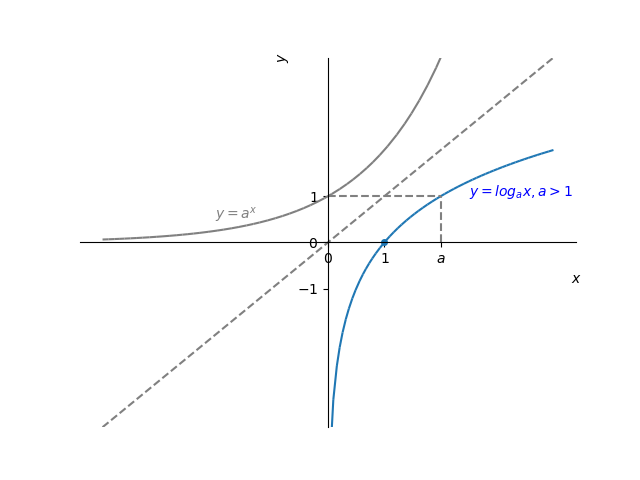
\includegraphics[width=0.5\textwidth]{./cap_funcao/dados/fig_log_graficos/fig_log_2}~
  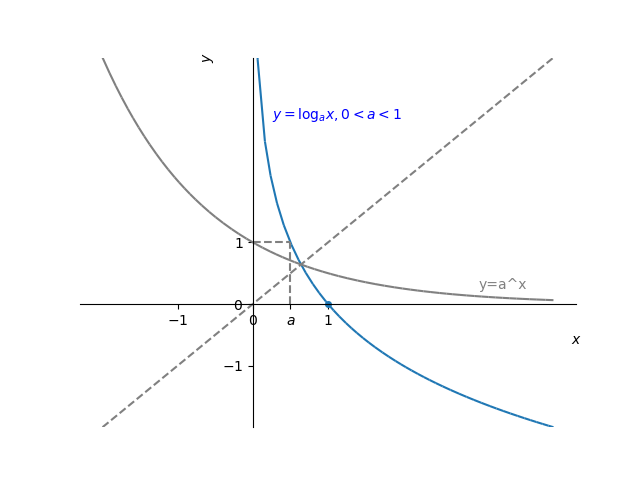
\includegraphics[width=0.5\textwidth]{./cap_funcao/dados/fig_log_graficos/fig_log_12}
  \caption{Esboços dos gráficos de funções logarítmicas: (esquerda) $y = \log_a x$, $a>1$; (direita) $y = \log_a x$, $0<a<1$.}
  \label{fig:log_graficos}
\end{figure}

\begin{obs}
  Quando a base é o número de Euler $e \approx 2,718281828459045$, chamamos $y = \log_e x$ de função exponencial natural e denotamo-la por $y = \ln x$.

  \ifispython
  No \sympy, podemos computar $\log_a x$ com a função \verb+log(x,a)+. O $\ln x$ é computado com $\verb+log(x)+$.
  \fi
\end{obs}

\begin{obs}
  Vejamos algumas propriedades dos logaritmos:
  \begin{itemize}
  \item $\displaystyle \log_a x = y \Leftrightarrow a^y = x$;
  \item $\displaystyle \log_a 1 = 0$;
  \item $\displaystyle \log_a a = 1$;
  \item $\displaystyle \log_a a^x = x$;
  \item $\displaystyle a^{\log_a^x} = x$;
  \item $\displaystyle \log_a xy = \log_a x + \log_a y$;
  \item $\displaystyle \log_a \frac{x}{y} = \log_a x - \log_a y$;
  \item $\displaystyle \log_a x^r = r\cdot\log_a x$.
  \item $\displaystyle \log_a x = \frac{\log_b x}{\log_b a}$
  \end{itemize}
\end{obs}

\subsection*{Exercícios resolvidos}

\begin{flushright}
  [Vídeo] | [Áudio] | \href{https://phkonzen.github.io/notas/contato.html}{[Contatar]}
\end{flushright}

\begin{exeresol}
  Faça o esboço do gráfico de $f(x) = \ln(x+2)+1$ e determine seu domínio.
\end{exeresol}
\begin{resol}
  Para fazermos o esboço do gráfico de $f(x) = \ln(x+2)+1$, podemos começar com o gráfico de $f_1(x) = \ln x$. Então, podemos transladá-lo 2 unidades à esquerda, de forma a obtermos $f_2(x) = \ln(x+2) = f_1(x+2)$. Por fim, transladamos o gráfico de $f_2(x)$ uma unidade para cima, obtendo o esboço do gráfico de $f(x) = \ln(x+2)+1=f_2(x)+1$. Veja a Figura \ref{fig:exeresol_lograf}.

  \begin{figure}[H]
    \centering
    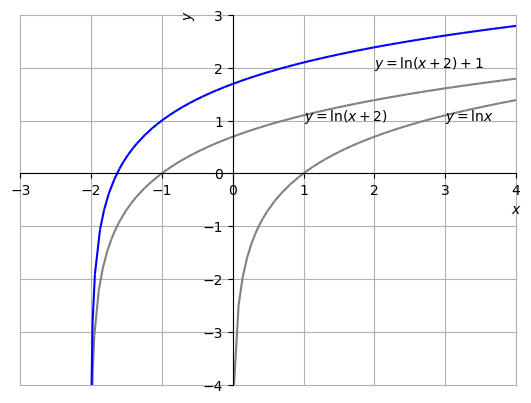
\includegraphics[width=0.5\textwidth]{./cap_funcao/dados/fig_exeresol_lograf/fig_exeresol_lograf}
    \caption{Esboço do gráfico de $f(x) = \ln(x+2)+1$.}
    \label{fig:exeresol_lograf}
  \end{figure}

Ainda, o domínio de $\ln x$ é $(0, \infty)$. Como, $f(x) = \ln(x+2)+1$ é uma translação de duas unidades à esquerda e uma para cima de $\ln x$, temos que o domínio de $f(x)$ é $(-2, \infty)$.
\end{resol}

\begin{exeresol}
  Resolva a seguinte equação para $x$
  \begin{equation}
    \ln(x+2) + 1 = 1. 
  \end{equation}
\end{exeresol}
\begin{resol}
  Podemos calcular a solução pelos seguintes passos:
  \begin{align}
    \ln(x+2)+1=1 &\Rightarrow \ln(x+2)=0\\
                 &\Rightarrow x+2=e^0\\
                 &\Rightarrow x=1-2=-1.\\
  \end{align}

  \ifispython
  Com o \sympy, podemos computar a solução com o seguinte comando:
\begin{verbatim}
solve(Eq(log(x+2)+1,1),x)
\end{verbatim}
  \fi
\end{resol}

\subsection*{Exercícios}

\begin{flushright}
  [Vídeo] | [Áudio] | \href{https://phkonzen.github.io/notas/contato.html}{[Contatar]}
\end{flushright}

\begin{exer}
  Faça o esboço do gráfico de $f(x) = \log(x-2)-1$ e determine seu domínio.
\end{exer}
\begin{resp}
  Dica: use um pacote computacional de matemática simbólica para verificar o esboço de seu gráfico. Domínio: $(2, \infty)$.
\end{resp}

\begin{exer}
  Resolva a seguinte equação para $x$
  \begin{equation}
    \ln(x+1)^2=0.
  \end{equation}
\end{exer}
\begin{resp}
  $0$
\end{resp}

%Este trabalho está licenciado sob a Licença Atribuição-CompartilhaIgual 4.0 Internacional Creative Commons. Para visualizar uma cópia desta licença, visite http://creativecommons.org/licenses/by-sa/4.0/deed.pt_BR ou mande uma carta para Creative Commons, PO Box 1866, Mountain View, CA 94042, USA.

\chapter{Limites}\label{cap_lim}
\thispagestyle{fancy}

\section{Noção de limites}\label{cap_lim_sec_lim}

\begin{flushright}
  \href{https://youtu.be/OxqOaaEIOjo}{[YouTube]} | \href{https://archive.org/details/nocaolim}{[Vídeo]} | [Áudio] | \href{https://phkonzen.github.io/notas/contato.html}{[Contatar]}
\end{flushright}

Seja $f$ uma função definida em um intervalo aberto em torno de um dado ponto $x_0$, exceto talvez em $x_0$. Quando o valor de $f(x)$ é {\bf arbitrariamente próximo} de um número $L$ para $x$ {\bf suficientemente próximo} de $x_0$, escrevemos
\begin{equation}
  \lim_{\color{blue}x\to x_0} f(x) = {\color{red}L}
\end{equation}
e dizemos que o {\bf limite da função $f$ é $L$ quando $x$ tende a $x_0$}. Veja a Figura \ref{fig:lim}.

\begin{figure}[H]
  \centering
  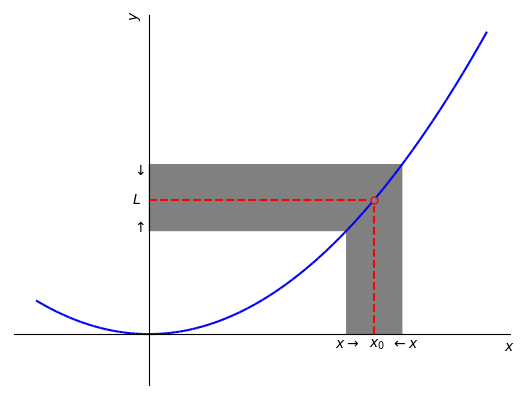
\includegraphics[width=0.7\textwidth]{./cap_lim/dados/fig_lim/fig_lim}
  \caption{Ilustração da noção de limite de uma função.}
  \label{fig:lim}
\end{figure}

\begin{ex}\label{ex:lim0}
  Consideremos a função
  \begin{equation}
    f(x) = \frac{(x^2-1)(x-2)}{(x-1)(x-2)}.
  \end{equation}
  Na Figura \ref{fig:ex_lim0}, temos um esboço do gráfico desta função.

  \begin{figure}[H]
    \centering
    \includegraphics[width=0.7\textwidth]{./cap_lim/dados/fig_ex_lim0/fig_ex_lim0}
    \caption{Esboço do gráfico da função $f(x)$ dada no Exemplo \ref{ex:lim0}.}
    \label{fig:ex_lim0}
  \end{figure}


  Vejamos os seguintes casos:
  \begin{itemize}
  \item $\displaystyle \lim_{x\to 0} f(x) = 1 = f(0)$.
    
    \begin{tabular}{r|ccc|c|ccc}
      $x$ & $-0,01$ & $-0,001$ & $-0,0001$ & $\rightarrow 0 \leftarrow$ & $0,0001$ & $0,001$ & $0,01$\\\hline
      $f(x)$ & $0,99$ & $0,999$ & $0,9999$ & $\rightarrow 1 \leftarrow$ & $1,0001$ & $1,001$ & $1,01$
    \end{tabular}

    \ifispython
    Com o {\python}+{\sympy}, podemos computar este limite com o comando
    \begin{lstlisting}
      In : from sympy import *
      ...: x = Symbol('x')
      ...: f = Lambda(x, (x**2-1)*(x-2)/ \
      ...:            ((x-1)*(x-2)))
      ...: limit(f(x), x, 0)
      Out: 1
    \end{lstlisting}
    \fi
  \item $\displaystyle \lim_{x\to 1} f(x) = 2$, embora $f(1)$ não esteja definido.
    
    \begin{tabular}{r|ccc|c|ccc}
      $x$ & $0,9$ & $0,99$ & $0,999$ & $\rightarrow 1 \leftarrow$ & $1,0001$ & $1,001$ & $1,01$\\\hline
      $f(x)$ & $1,9$ & $1,99$ & $1,999$ & $\rightarrow 2 \leftarrow$ & $2,0001$ & $2,001$ & $2,01$
    \end{tabular}
  \item $\displaystyle \lim_{x\to 2} f(x) = 3$, embora $f(2)$ também não esteja definido. Verifique!
  \end{itemize}
\end{ex}

\subsection{Limites da função constante e da função identidade}\label{sslfc}

\begin{flushright}
  \href{https://youtu.be/_7YiqVx8e8M}{[YouTube]} | \href{https://archive.org/details/lim_fconst_fid}{[Vídeo]} | [Áudio] | \href{https://phkonzen.github.io/notas/contato.html}{[Contatar]}
\end{flushright}

Da noção de limite, podemos inferir que
\begin{equation}
  \lim_{x\to x_0} k = k,
\end{equation}
seja qual for a constante $k$. Veja a Figura \ref{fig:lim_funk}.

\begin{figure}[H]
  \centering
  \includegraphics[width=0.7\textwidth]{./cap_lim/dados/fig_lim_funk/fig_lim_funk}
  \caption{Esboço do gráfico de uma função constante $f(x) = k$.}
  \label{fig:lim_funk}
\end{figure}

\begin{ex}
  Vejamos os seguintes casos:
  \begin{enumerate}[a)]
  \item $\displaystyle \lim_{x\to -1} 1 = 1$
    \ifispython
    No {\python}, podemos computar este limite com os seguintes comandos.
    \begin{lstlisting}
      In : from sympy import *
      ...: x = Symbol("x")
      ...: limit(1, x, -1)
      ...: 
      Out: 1
    \end{lstlisting}
    \fi
  \item $\displaystyle \lim_{x\to 2} -3 = -3$
  \item $\displaystyle \lim_{x\to \pi} \left(\sqrt{2} - e\right) = \sqrt{2}-e$
  \end{enumerate}
\end{ex}

Também da noção de limites, podemos inferir que
\begin{equation}
  \lim_{x\to x_0} x = x_0,
\end{equation}
seja qual for o ponto $x_0$. Vejamos a Figura \ref{fig:lim_funid}.

\begin{figure}[H]
  \centering
  \includegraphics[width=0.7\textwidth]{./cap_lim/dados/fig_lim_funid/fig_lim_funid}
  \caption{Noção de limite para a função identidade $f(x)=x$.}
  \label{fig:lim_funid}
\end{figure}

\begin{ex}
  Vejamos os seguintes casos:
  \begin{enumerate}[a)]
  \item $\displaystyle \lim_{x\to -1} x = -1$
    \ifispython
    Com o {\python}, podemos computar este limite com os seguintes comandos.
    \begin{lstlisting}
      In : from sympy import *
      ...: x = Symbol("x")
      ...: limit(x, x, -1)
      ...: 
      Out: -1
    \end{lstlisting}
    \fi
  \item $\displaystyle \lim_{x\to 2} x = 2$
  \item $\displaystyle \lim_{x\to \pi} x = \pi$
  \end{enumerate}
\end{ex}

\subsection*{Exercícios resolvidos}

\begin{flushright}
  [Vídeo] | [Áudio] | \href{https://phkonzen.github.io/notas/contato.html}{[Contatar]}
\end{flushright}

\begin{exeresol}
  Estime o valor do limite
  \begin{equation}
    \lim_{x\to 1} e^x.
  \end{equation}
\end{exeresol}
\begin{resol}
  Da noção de limite, podemos buscar inferir o limite de uma função em um ponto $x_0$, computando seus valores próximos deste ponto. Por exemplo, construímos a seguinte tabela:
  
  \begin{tabular}{r|ccc|c|ccc}
    $x$ & $0,9$ & $0,99$ & $0,999$ & $\rightarrow 1 \leftarrow$ & $1,0001$ & $1,001$ & $1,01$\\\hline
    $f(x)$ & $2,460$ & $2,691$ & $2,716$ & $\rightarrow 2,72 \leftarrow$ & $2,719$ & $2,721$ & $2,746$
  \end{tabular}
  
  Com isso, inferimos que
  \begin{equation}
    \lim_{x\to 1} e^x \approx 2,72.
  \end{equation}
  Mais adiante, veremos que $\lim_{x\to 1} e^x = e \approx 2,718281828459045 ...$.
  
  \ifispython
  Verifique usando {\python}+{\sympy}!
  \fi
\end{resol}

\begin{exeresol}
  Considere que uma dada função $f$ tenha o seguinte esboço de gráfico:

  \begin{center}
    \includegraphics[width=0.7\textwidth]{./cap_lim/dados/fig_exeresol_nocaolim/fig_exeresol_nocaolim}
  \end{center}

  Então, infira o valores de
  \begin{enumerate}[a)]
  \item $\displaystyle \lim_{x\to -2} f(x)$
  \item $\displaystyle \lim_{x\to -1} f(x)$
  \item $\displaystyle \lim_{x\to 1} f(x)$
  \end{enumerate}
\end{exeresol}
\begin{resol}
  \begin{enumerate}[a)]
  \item $\displaystyle \lim_{x\to -2} f(x)$

    Para valores suficientemente próximos de $-2$ e a direita de $-2$ (i.e. $x>-2$), podemos observar que $f(x)=1$. Para tais valores de $x$ a esquerda de $-2$ (i.e. $x<-2$), vemos que os valores de $f(x)$ tornam-se próximos de $1$. Isto é, temos que os valores de $f(x)$ podemos ser tomados arbitrariamente próximos de $L=1$, se tomarmos $x$ suficientemente próximo de $-2$. Concluímos que
    \begin{equation}
      \lim_{x\to -2} = 1.
    \end{equation}

  \item $\displaystyle \lim_{x\to -1} f(x)$

    Mesmo sendo $f(-1)=2$, observamos que os valores de $f(x)$ podem ser tomados arbitrariamente próximos de $1$, se escolhemos valores de $x$ suficientemente próximos de $-1$. Logo,
    \begin{equation}
      \lim_{x\to -1} f(x) = 1.
    \end{equation}

    \item $\displaystyle \lim_{x\to 1} f(x)$

      Aqui, para valores de $x$ suficientemente próximos de $x_0=1$ e a esquerda ($x<1$), vemos que os valores de $f(x)$ são próximos de $L=2$. Entretanto, para valores de $x$ suficientemente próximos de $x_0=1$ e a direita ($x>1$), temos que os valores de $f(x)$ são próximos de $L=1$. Ou seja, não é possível escolher um valor $L$ tal que $f(x)$ esteja arbitrariamente próxima ao tomarmos $x$ suficientemente próximo de $x_0=1$, pois $L$ dependerá de $x$ estar a esquerda ou a direita de do ponto $x_0 = 1$. Concluímos que este limite não existe, e escrevemos
      \begin{equation}
        \not\exists\lim_{x\to 1} f(x).
      \end{equation}
  \end{enumerate}
\end{resol}

\subsection*{Exercícios}

\begin{flushright}
  [Vídeo] | [Áudio] | \href{https://phkonzen.github.io/notas/contato.html}{[Contatar]}
\end{flushright}

\begin{exer}\label{exer:limgraf}
  Considere que uma dada função $f$ tenha o seguinte esboço de gráfico:
  \includegraphics[width=0.8\textwidth]{./cap_lim/dados/fig_exer_limgraf/fig_exer_limgraf}

  Forneça o valor dos seguintes limites:
  \begin{enumerate}[a)]
  \item $\displaystyle \lim_{x\to -1} f(x)$
  \item $\displaystyle \lim_{x\to 1} f(x)$
  \item $\displaystyle \lim_{x\to 2} f(x)$
  \item $\displaystyle \lim_{x\to 3} f(x)$
  \end{enumerate}
\end{exer}
\begin{resp}
  a)~$-1$; b)~$-1$; c)~$2$; d)~$\nexists$
\end{resp}

\begin{exer}
  Considerando a mesma função do exercício anterior (Exercício \ref{exer:limgraf}), forneça
  \begin{enumerate}
  \item $\displaystyle \lim_{x\to -\frac{3}{2}} f(x)$
  \item $\displaystyle \lim_{x\to 0} f(x)$
  \item $\displaystyle \lim_{x\to \frac{3}{4}} f(x)$
  \end{enumerate}
\end{exer}
\begin{resp}
  a)~$-\frac{3}{2}$; b)~$-1$; c)~$-1$
\end{resp}

\begin{exer}
  Forneça o valor dos seguintes limites:
  \begin{enumerate}[a)]
  \item $\displaystyle \lim_{x\to 2} 2$
  \item $\displaystyle \lim_{x\to -2} 2$
  \item $\displaystyle \lim_{x\to 2} -3$
  \item $\displaystyle \lim_{x\to e} \pi$
  \end{enumerate}
\end{exer}
\begin{resp}
  a)~2; b)~2; c)~-3; d)~$\pi$
\end{resp}

\begin{exer}
  Forneça o valor dos seguintes limites:
  \begin{enumerate}[a)]
  \item $\displaystyle \lim_{x\to 2} x$
  \item $\displaystyle \lim_{x\to -2} x$
  \item $\displaystyle \lim_{x\to -3} x$
  \item $\displaystyle \lim_{x\to e} x$
  \end{enumerate}
\end{exer}
\begin{resp}
  a)~2; b)~-2; c)~-3; d)~$e$
\end{resp}

\begin{exer}
  Com base na noção de limites, calcule:
  \begin{enumerate}[a)]
  \item $\displaystyle\lim_{x\to 1} |x|$
  \item $\displaystyle\lim_{x\to -1} |x|$
  \item $\displaystyle\lim_{x\to 10^{-10}} |x|$
  \end{enumerate}
\end{exer}
\begin{resp}
  a) $1$; b) $1$; c) $10^{-10}$
\end{resp}

\section{Regras para o cálculo de limites}\label{cap_lim_sec_regras}

\subsection{Regras de cálculo}

\begin{flushright}
  \href{https://youtu.be/chAoC7xoeYM}{[YouTube]} | \href{https://archive.org/details/video_20220629_1213}{[Vídeo]} | [Áudio] | \href{https://phkonzen.github.io/notas/contato.html}{[Contatar]}
\end{flushright}

Sejam dados os seguintes limites
\begin{gather}
  \lim_{x\to x_0} f(x) = L_1\\
  \lim_{x\to x_0} g(x) = L_2
\end{gather}
com $x_0, L_1, L_2$ números reais. Então, valem as seguintes regras:
\begin{itemize}
\item Regra da multiplicação por um escalar:
  \begin{align}
    \lim_{x\to x_0} k\cdot f(x) &= k\cdot \lim_{x\to x_0} f(x)\\
                          &= k\cdot L_1,
  \end{align}
  para qualquer número real $k$.
\item Regra da soma/subtração:
  \begin{align}
    \lim_{x\to x_0} f(x) \pm g(x) &= \lim_{x\to x_0} f(x) \pm \lim_{x\to x_0} g(x) \\
                                  &= L_1 \pm L_2
  \end{align}
\item Regra do produto:
  \begin{align}
    \lim_{x\to x_0} f(x) \cdot g(x) &= \lim_{x\to x_0} f(x) \cdot \lim_{x\to x_0} g(x) \\
                                    &= L_1 \cdot L_2
  \end{align}
\item Regra do quociente:
  \begin{align}
    \lim_{x\to x_0} \frac{f(x)}{g(x)} &= \frac{\lim_{x\to x_0} f(x)}{\lim_{x\to x_0} g(x)} \\
    &= \frac{L_1}{L_2},\qquad L_2\neq 0
  \end{align}
\item Regra da potenciação:
  \begin{align}
    \lim_{x\to x_0} (f(x))^s &= \left(\lim_{x\to x_0} f(x)\right)^s\\
    &= L_1^s,\qquad L_1^s\in\mathbb{R}
  \end{align}
\end{itemize}

Podemos usar essas regras para calcularmos limites.

\begin{ex}
  Consideremos os seguintes casos:
  \begin{enumerate}[a)]
  \item $\displaystyle \lim_{x\to -1} 2x$
  \begin{align}
    \lim_{x\to -1} 2x &= 2\lim_{x\to -1} x\\
    &= 2\cdot(-1) = -2
  \end{align}
  \ifispython
  Com o {\python}+{\sympy}, podemos computar este limite com
  \begin{lstlisting}
    from sympy import *
    x = Symbol("x")
    limit(2*x,x,-1)
  \end{lstlisting}
  \fi
\item $\displaystyle \lim_{x\to 2} x^2 - 1$
  \begin{align}
    \lim_{x\to 2} x^2 - 1 &= \lim_{x\to 2} x^2 - \lim_{x\to 2} 1\\
                          &= \left(\lim_{x\to 2} x\right)^2 - 1\\
                          &= 2^2 - 1 = 3.
  \end{align}
  \ifispython
  Com o {\python}+{\sympy}, podemos computar este limite com os seguintes comandos.
  \begin{lstlisting}
    from sympy import *
    x = Symbol("x")
    limit(x**2-1,x,2)
  \end{lstlisting}
  \fi
\item $\displaystyle \lim_{x\to 0} \sqrt{1-x^2}$.
  \begin{align}
    \lim_{x\to 0} \sqrt{1-x^2} &= \sqrt{\lim_{x\to 0} 1-x^2}\\
                                &= \sqrt{\lim_{x\to 0} 1 - \left(\lim_{x\to 0} x\right)^2}\\
                                &= \sqrt{1 - (0)^2} \\
                                &= 1.
  \end{align}
  \ifispython
  Com o {\python}+{\sympy}, podemos computar este limite com
  \begin{lstlisting}
    from sympy import *
    x = Symbol("x")
    limit(sqrt(1-x**2),x,0)
  \end{lstlisting}
  \fi  
\item $\displaystyle \lim_{x\to 0} \frac{(x^2-1)(x-2)}{(x-1)(x-2)}$
  \begin{align}
    \lim_{x\to 0} \frac{(x^2-1)(x-2)}{(x-1)(x-2)} &= \frac{\displaystyle\lim_{x\to 0}\left[(x^2-1)\cdot(x-2)\right]}{\displaystyle\lim_{x\to 0} \left[(x-1)\cdot(x-2)\right]}\\
                                                  &= \frac{\displaystyle\lim_{x\to 0} (x^2-1)\cdot\lim_{x\to 0}(x-2)}{\displaystyle\lim_{x\to 0}(x-1)\cdot\lim_{x\to 0}(x-2)}\\
    &= \frac{2}{2} = 1.
  \end{align}
  \end{enumerate}
\end{ex}

\begin{prop}\normalfont{(Limites de polinômios)}\label{prop:lim_poli}
  Se
  \begin{equation}
    p(x) = a_nx^n + a_{n-1}x^{n-1} + \cdots + a_0,
  \end{equation}
  então
  \begin{align}
    \lim_{x\to b} p(x) &= p(b)\\
                       &= a_nb^n + a_{n-1}b^{n-1} + \cdots + a_0,
  \end{align}
  para qualquer dado número real $b$.
\end{prop}
\begin{dem}
  Segue das regras da soma, da multiplicação por escalar e da potenciação.
  \begin{align}
    \lim_{x\to b} p(x) &= \lim_{x\to b} a_nx^n + a_{n-1}x^{n-1} + \cdots + a_0\\
                       &= \lim_{x\to b} a_nx^n + \lim_{x\to b} a_{n-1}x^{n-1} + \cdots + \lim_{x\to b} a_0\\
                       &= a_n\left(\lim_{x\to b} x\right)^n + a_{n-1}\left(\lim_{x\to b} x\right)^{n-1} + \cdots + a_0\\
                       &= a_nb^n + a_{n-1}b^{n-1} + \cdots + a_0 = p(b).
  \end{align}
\end{dem}

\begin{ex}
  \begin{align}
    \lim_{x\to \sqrt{2}} 2x^4 - 2x^2 + x &= 2(\sqrt{2})^4 - 2(\sqrt{2})^2 + \sqrt{2}\\
                                         &= 4+\sqrt{2}.
  \end{align}
  \ifispython
  Com o {\python}+{\sympy}, podemos computar este limite com os seguintes comandos.
  \begin{lstlisting}
    from sympy import *
    x = Symbol("x")
    limit(2*x**4-2*x**2+x,x,sqrt(2))
  \end{lstlisting}
  \fi
\end{ex}

\begin{prop}\normalfont{(Limite de funções racionais)}
  Sejam $r(x) = p(x)/q(x)$ uma função racional e $b$ um número real tal que $q(b)\neq 0$. Então,
  \begin{equation}
    \lim_{x\to b} \frac{p(x)}{q(x)} = \frac{p(b)}{q(b)}.
  \end{equation}
\end{prop}
\begin{dem}
  Segue da regra do \emph{limite do quociente} e da Proposição \ref{prop:lim_poli}.
  \begin{align}
    \lim_{x\to b} \frac{p(x)}{q(x)} &= \frac{\displaystyle\lim_{x\to b} p(x)}{\displaystyle\lim_{x\to b} q(x)} \\
                                    &= \frac{p(b)}{q(b)}.
  \end{align}
\end{dem}

\begin{ex}
  \begin{align}
    \lim_{x\to 0} \frac{(x^2-1)(x-2)}{(x-1)(x-2)} &= \frac{(0^2-1)(0-2)}{(0-1)(0-2)}\\
                                                  &= \frac{2}{2} = 1.
  \end{align}
  \ifispython
  Com o {\python}+{\sympy}, podemos computar este limite com os comandos.
  \begin{lstlisting}
    from sympy import *
    x = Symbol("x")
    limit((x**2-1)*(x-2)/((x-1)*(x-2)),x,0)
  \end{lstlisting}
  \fi
\end{ex}

\subsection{Indeterminação $0/0$}

\begin{flushright}
  \href{https://youtu.be/dW3CfM2JjKY}{[YouTube]} | \href{https://archive.org/details/video_20220701_1415}{[Vídeo]} | [Áudio] | \href{https://phkonzen.github.io/notas/contato.html}{[Contatar]}
\end{flushright}

Quando $\displaystyle \lim_{x\to a} f(a)=0$ e $\displaystyle \lim_{x\to a} g(a)=0$, dizemos que
\begin{equation}
  \lim_{x\to a} \frac{f(x)}{g(x)}
\end{equation}
é uma {\bf indeterminação do tipo $0/0$}. Em vários destes casos, podemos calcular o limite eliminando o fator em comum $(x-a)$.

\begin{ex}
  \begin{align}
    \lim_{x\to 2}\frac{(x^2-1)\cancel{(x-2)}}{(x-1)\cancel{(x-2)}} &= \lim_{x\to 2} \frac{x^2-1}{x-1}\\
                                                                   &= \frac{2^2-1}{2-1} = 3.
  \end{align}
  \ifispython
  Com o {\python}+{\sympy}, podemos computar o limite acima com os seguintes comandos.
  \begin{lstlisting}
    from sympy import *
    x = Symbol("x")
    limit((x**2-1)*(x-2)/((x-1)*(x-2)),x,2)
  \end{lstlisting}
  \fi
\end{ex}

Quando o fator em comum não aparece explicitamente, podemos tentar trabalhar algebricamente de forma a explicitá-lo.

\begin{ex}
  No caso do limite
  \begin{align}
    \lim_{x\to 1} \frac{x^3-3x^2-x+3}{x^2+x-2}
  \end{align}
  temos que o denominador $p(x) = x^3-3x^2-x+3$ se anula em $x=1$, assim como o denominador $q(x) = x^2+x-2$. Assim sendo, $(x-1)$ é um fator comum entre $p(x)$ e $q(x)$. Para explicitá-lo, calculamos
  \begin{align}
    \frac{p(x)}{x-1} &= \frac{x^3-3x^2-x+3}{x-1}\\
                     &= x^2-2x-3
  \end{align}
  e
  \begin{align}
    \frac{q(x)}{x-1} &= \frac{x^2+x-2}{x-1}\\
                     &= x+2.
  \end{align}
  \ifispython
  Com o {\python}+{\sympy}, podemos computar estas divisões com os seguintes comandos.
  \begin{lstlisting}
    from sympy import *
    x = Symbol("x")
    simplify((x**3-3*x**2-x+3)/(x-1))
    simplify((x**2+x-2)/(x-1))
  \end{lstlisting}
  \fi
  Realizadas as divisões, temos
  \begin{equation}
    p(x) = (x-1)(x^2-2x-3)
  \end{equation}
  e
  \begin{equation}
    q(x)=(x-1)(x+2).
  \end{equation}
  Com isso, segue que
  \begin{align}
    \lim_{x\to 1} \frac{x^3-3x^2-x+3}{x^2+x-2} &= \lim_{x\to 1} \frac{(x-1)(x^2-2x-3)}{(x-1)(x+2)} \\
    &= \lim_{x\to 1} \frac{x^2-2x-3}{x+2} = -\frac{4}{3}.
  \end{align}
  \ifispython
  Use {\python}+{\sympy} para computar este limite!
  \fi
\end{ex}

\begin{ex}
  No caso de
  \begin{equation}
    \lim_{x\to 0} \frac{\sqrt{1-x}-1}{x}
  \end{equation}
  temos uma indeterminação do tipo $0/0$ envolvendo uma raiz. Neste caso, podemos calcular o limite usando de racionalização.
  \begin{align}
    \lim_{x\to 0} \frac{\sqrt{1-x}-1}{x} &= \lim_{x\to 0} \frac{\sqrt{1-x}-1}{x}\frac{\sqrt{1-x}+1}{\sqrt{1-x}+1}\\
                                         &= \lim_{x\to 0} \frac{1-x-1}{x(\sqrt{1-x}+1)} \\
                                         &- \lim_{x\to 0} \frac{-x}{x(\sqrt{1-x}+1)}\\
    &= \lim_{x\to 0} \frac{-1}{\sqrt{1-x}+1} = -\frac{1}{2}.
  \end{align}
  \ifispython
  Verifique computando com o {\python}+{\sympy}. 
  \fi
\end{ex}

\subsection*{Exercícios resolvidos}

\begin{flushright}
  [Vídeo] | [Áudio] | \href{https://phkonzen.github.io/notas/contato.html}{[Contatar]}
\end{flushright}

\begin{exeresol}
  Calcule
  \begin{equation}
    \lim_{x\to -1} \frac{x - x^2}{\sqrt{x^2+3}}.
  \end{equation}
\end{exeresol}
\begin{resol}
  Usando das propriedades de limites, calculamos
  \begin{align}
    \lim_{x\to -1} \frac{x-x^2}{\sqrt{x^2+3}} &= \frac{\displaystyle\lim_{x\to -1} x-x^2}{\displaystyle\lim_{x\to -1} \sqrt{x^2+3}} \\
                                              &= \frac{-1-(-1)^2}{\displaystyle\sqrt{\lim_{x\to -1} x^2+3}} \\
                                              &= \frac{-2}{\sqrt{4}} \\
                                              &= -1.
  \end{align}
\end{resol}

\begin{exeresol}
  Assumindo que o $\lim_{x\to 2} f(x) = L$ e que
  \begin{equation}
    \lim_{x\to 2} \frac{f(x)-2}{x+2} = 1,
  \end{equation}
  forneça o valor de $L$.
\end{exeresol}
\begin{resol}
  Das propriedades de limites, temos
  \begin{gather}
    \lim_{x\to 2} \frac{f(x)-2}{x+2} = 1\\
    \frac{\displaystyle\lim_{x\to 2} f(x)-2}{\displaystyle\lim_{x\to 2} x+2} = 1\\
    \frac{\lim_{x\to 2} f(x) - \lim_{x\to 2} 2}{2+2} = 1\\
    \frac{L-2}{4} = 1\\
    L-2 = 4\\
    L = 6.
  \end{gather}
\end{resol}


\begin{exeresol}
  Calcule
  \begin{equation}
    \lim_{x\to -1} \frac{x+1}{2-\sqrt{x^2+3}}.
  \end{equation}
\end{exeresol}
\begin{resol}
  Neste caso, não podemos usar a regra do quociente, pois
  \begin{equation}
    \lim_{x\to -1} 2-\sqrt{x^2+3} = 0.
  \end{equation}
  Agora, como também temos
  \begin{equation}
    \lim_{x\to -1} x+1 = 0,
  \end{equation}
  concluímos se tratar de uma indeterminação $0/0$. Por racionalização, obtemos
  \begin{align}
    \lim_{x\to -1} \frac{x+1}{2-\sqrt{x^2+3}} &= \lim_{x\to -1} \frac{x+1}{2-\sqrt{x^2+3}}\frac{2+\sqrt{x^2+3}}{2+\sqrt{x^2+3}} \\
                                              &= \lim_{x\to -1} \frac{(x+1)(2+\sqrt{x^2+3})}{4 - (x^2+3)}\\
                                              &= \lim_{x\to -1} \frac{(x+1)(2+\sqrt{x^2+3})}{1-x^2}\\
                                              &= \lim_{x\to -1} \frac{(x+1)(2+\sqrt{x^2+3})}{(1+x)(1-x)}\\
                                              &= \lim_{x\to -1} \frac{2+\sqrt{x^2+3}}{1-x} \\
                                              &= \frac{4}{2} = 2.
  \end{align}
\end{resol}

\subsection*{Exercícios}

\begin{flushright}
  [Vídeo] | [Áudio] | \href{https://phkonzen.github.io/notas/contato.html}{[Contatar]}
\end{flushright}

\begin{exer}
  Sabendo que
  \begin{equation}
    \lim_{x\to -2} f(x) = 2,
  \end{equation}
  calcule:
  \begin{enumerate}[a)]
  \item $\displaystyle \lim_{x\to -2} 2\cdot f(x)$.
  \item $\displaystyle \lim_{x\to -2} \pi\cdot f(x)$.
  \item $\displaystyle \lim_{x\to -2} -e^{\sqrt{2}}\cdot f(x)$.
  \end{enumerate}
\end{exer}
\begin{resp}
  a)~$4$; b)~$2\pi$; c)~$-2e^{\sqrt{2}}$
\end{resp}

\begin{exer}
  Considerando que
  \begin{equation}
    \lim_{x\to 3} f(x) = -2
  \end{equation}
  e
  \begin{equation}
    \lim_{x\to 3} g(x) = \frac{1}{2},
  \end{equation}
  calcule:
  \begin{enumerate}[a)]
  \item $\displaystyle\lim_{x\to 3} f(x)+g(x)$
  \item $\displaystyle\lim_{x\to 3} g(x)-f(x)$
  \item $\displaystyle\lim_{x\to 3} f(x)-2g(x)$
  \end{enumerate}
\end{exer}
\begin{resp}
  a)~$-3/2$; b)~$5/2$; c)~$-3$
\end{resp}

\begin{exer}
  Considerando que
  \begin{equation}
    \lim_{x\to 0} f(x) = 3
  \end{equation}
  e
  \begin{equation}
    \lim_{x\to 0} g(x) = -2,
  \end{equation}
  calcule:
  \begin{enumerate}[a)]
  \item $\displaystyle\lim_{x\to 0} f(x)\cdot g(x)$
  \item $\displaystyle\lim_{x\to 0} g(x)\cdot (\frac{1}{2}\cdot f(x))$
  \end{enumerate}
\end{exer}
\begin{resp}
  a)~$-6$; b)~$-3$;
\end{resp}

\begin{exer}
  Considerando que
  \begin{equation}
    \lim_{x\to 0} f(x) = -2
  \end{equation}
  e
  \begin{equation}
    \lim_{x\to 0} g(x) = -3,
  \end{equation}
  calcule:
  \begin{enumerate}[a)]
  \item $\displaystyle\lim_{x\to 0} \frac{f(x)}{g(x)}$
  \item $\displaystyle\lim_{x\to 0} \frac{g(x)}{2f(x)}$
  \end{enumerate}
\end{exer}
\begin{resp}
  a)~$2/3$; b)~$3/4$;
\end{resp}

\begin{exer}
  Considerando que
  \begin{equation}
    \lim_{x\to -1} f(x) = -1
  \end{equation}
  e
  \begin{equation}
    \lim_{x\to -1} g(x) = 4,
  \end{equation}
  calcule:
  \begin{enumerate}[a)]
  \item $\displaystyle\lim_{x\to -1} \sqrt{g(x)}$
  \item $\displaystyle\lim_{x\to -1} \sqrt[3]{f(x)}$
  \item $\displaystyle\lim_{x\to -1} (f(x))^{\frac{4}{3}}$
  \end{enumerate}
\end{exer}
\begin{resp}
  a)~$2$; b)~$-1$; c)~$1$
\end{resp}

\begin{exer}
  Calcule os limites:
  \begin{enumerate}[a)]
  \item $\displaystyle\lim_{x\to -2} -3x$\\
  \item $\displaystyle\lim_{x\to -2} x^2-3x$\\    
  \item $\displaystyle\lim_{x\to -2} x^2-3x+\sqrt{x^2}$\\    
  \end{enumerate}
\end{exer}
\begin{resp}
  a)~$6$; b)~$10$; c)~$12$
\end{resp}

\begin{exer}
  Calcule os limites:
  \begin{enumerate}[a)]
  \item $\displaystyle\lim_{x\to -1} \frac{x}{x-1}$\\
  \item $\displaystyle\lim_{x\to -1} \frac{x^2+x-2}{x^2-3x+2}$\\    
  \end{enumerate}
\end{exer}
\begin{resp}
  a)~$1/2$; b)~$-1/3$;
\end{resp}

\begin{exer}
  Calcule os limites:
  \begin{enumerate}[a)]
  \item $\displaystyle\lim_{x\to 1} \frac{x^2-1}{x-1}$\\
  \item $\displaystyle\lim_{x\to -1} \frac{x^2-1}{2x+2}$\\
  \item $\displaystyle\lim_{x\to 1} \frac{x^2+x-2}{x^2-3x+2}$\\    
  \end{enumerate}
\end{exer}
\begin{resp}
  a)~$2$; b)~$-1$; c)~$-3$;
\end{resp}

\begin{exer}
  Calcule o limite
  \begin{equation}
    \lim_{x\to 6} \frac{2-\sqrt{x-2}}{x-6}.
  \end{equation}
\end{exer}
\begin{resp}
  $-1/4$
\end{resp}

\begin{exer}
  Diga se é verdadeira ou falsa a seguinte afirmação. Se existem
  \begin{gather}
    \lim_{x\to 1} f(x) = L\\
    \lim_{x\to -1} g(x) = M
  \end{gather}
  então
  \begin{equation}
    \lim_{x\to 1} f(x) + g(x) = L + M.
  \end{equation}
  Justifique sua resposta.
\end{exer}
\begin{resp}
  Falso. Construa um contraexemplo para mostrar que a afirmação não é verdadeira. 
\end{resp}


\section{Limites laterais}\label{cap_lim_sec_lateral}

\begin{flushright}
  \href{https://youtu.be/BFJPIejdyZM}{[YouTube]} | \href{https://archive.org/details/video_20220708_1407}{[Vídeo]} | [Áudio] | \href{https://phkonzen.github.io/notas/contato.html}{[Contatar]}
\end{flushright}

Seja dada uma função $f$ definida para todo $x$ em um intervalo aberto $(a, x_0)$. O {\bf limite lateral à esquerda} de $f$ no ponto $x_0$ é denotado por
\begin{equation}
  \lim_{x\to {\color{red}x_0^-}} f(x)
\end{equation}
e é computado tendo em vista a tendência da função apenas para pontos $x<x_0$. Em outras palavras, o
\begin{equation}
  \lim_{x\to x_0^-} f(x) = L
\end{equation}
quando $f(x)$ é arbitrariamente próximo de $L$, para todo $x<x_0$ suficientemente próximo de $x_0$. Veja a Figura \ref{fig:lim_esq}.

\begin{figure}[H]
  \centering
  \includegraphics[width=0.7\textwidth]{./cap_lim/dados/fig_lim_esq/fig_lim_esq}
  \caption{Ilustração da noção de limite lateral à esquerda.}
  \label{fig:lim_esq}
\end{figure}

Para uma função $f$ definida para todo $x$ em um intervalo aberto $(x_0, b)$, o {\bf limite lateral à direita} de $f$ no ponto $x_0$ é denotado por
\begin{equation}
  \lim_{x\to {\color{blue}x_0^+}} f(x)
\end{equation}
e é computado tendo em vista a tendência da função apenas para pontos $x>x_0$. Em outras palavras, temos
\begin{equation}
  \lim_{x\to x_0^+} f(x) = L,
\end{equation}
quando $f(x)$ é arbitrariamente próximo de $L$, para todo $x>x_0$ suficientemente próximo de $x_0$. Veja a Figura \ref{fig:lim_dir}.

\begin{figure}[H]
  \centering
  \includegraphics[width=0.7\textwidth]{./cap_lim/dados/fig_lim_dir/fig_lim_dir}
  \caption{Ilustração da noção de limite lateral à direita.}
  \label{fig:lim_dir}
\end{figure}

\begin{obs}
  Por inferência direta, temos
  \begin{equation}
    \lim_{x\to x_0^{\pm}} k = k
  \end{equation}
  e
  \begin{equation}
    \lim_{x\to x_0^{\pm}} x = x_0,
  \end{equation}
  onde $x_0$ e $k$ são quaisquer dados números reais.
\end{obs}

\begin{exer}\label{ex:lim_absx}
  Vamos calcular
  \begin{equation}
    \lim_{x\to 0^-} |x|.
  \end{equation}
  Por definição, temos
  \begin{equation}
    |x| := \left\{
      \begin{array}{ll}
        x &, x\geq 0,\\
        -x &, x< 0.
      \end{array}
    \right.
  \end{equation}
  Como estamos interessados no limite lateral à esquerda de $x=0$, trabalhamos com $x<0$ e, então
  \begin{align}
    \lim_{x\to 0^-} |x| &= \lim_{x\to 0^-} -x\\
                        &= -\lim_{x\to 0^-} x = 0.
  \end{align}
  
  Analogamente, calculamos
  \begin{equation}
    \lim_{x\to 0^+} |x| = \lim_{x\to 0^+} x = 0.
  \end{equation}
  Verifique!

  \ifispython
  Com o {\python}+{\sympy}, podemos computar os limites acima com os seguintes comandos.
  \begin{lstlisting}
    from sympy import *
    x = Symbol("x")
    limit(abs(x),x,0,'-')
    limit(abs(x),x,0,'+')
  \end{lstlisting}
  \fi
\end{exer}

\begin{teo}\label{teo:lim_existe}
  Existe o limite de uma dada função $f$ no ponto $x=x_0$ e
  \begin{equation}
    \lim_{x\to x_0} f(x) = L
  \end{equation}
  se, e somente se, existem e são iguais a $L$ os limites laterais à esquerda e à direita de $f$ no ponto $x=x_0$.
\end{teo}

\begin{exer}
  No exemplo anterior (Exemplo \ref{ex:lim_absx}), vimos que
  \begin{equation}
    \lim_{x\to 0^-} |x| = \lim_{x\to 0^+} |x| = 0.
  \end{equation}
  Logo, pelo teorema acima (Teorema \ref{teo:lim_existe}), podemos concluir que
  \begin{equation}
    \lim_{x\to 0} |x| = 0.
  \end{equation}
\end{exer}

\begin{exer}
  Vamos verificar a existência de
  \begin{equation}
    \lim_{x\to 0} \frac{|x|}{x}.
  \end{equation}
  Começamos pelo limite lateral à esquerda, temos
  \begin{align}
    \lim_{x\to 0^-} \frac{|x|}{x} &= \lim_{x\to 0^-} \frac{-x}{x}\\
    &= \lim_{x\to 0^-} -1 = -1.
  \end{align}
  Agora, calculando o limite lateral à direta, obtemos
  \begin{align}
    \lim_{x\to 0^+} \frac{|x|}{x} &= \lim_{x\to 0^+} \frac{x}{x}\\
    &= \lim_{x\to 0^+} 1 = 1.
  \end{align}
  Como os \emph{limites laterais} à esquerda e à direita \emph{são diferentes}, concluímos que \emph{não existe o limite} de $|x|/x$ no ponto $x=0$.

  \ifispython
  Com o {\python}+{\sympy}, por padrão o limite computado é sempre o limite lateral à direita. É por isso que o comando
  \begin{lstlisting}
    from sympy import *
    x = Symbol("x")
    limit(abs(x)/x,x,0)
  \end{lstlisting}
  fornece o valor $1$ como saída.
  \fi
\end{exer}

\begin{obs}
  As regras básicas para o cálculo de limites bilaterais são estendidas para limites laterais. I.e., se
  \begin{equation}
    \lim_{x\to x_0^{\pm}} f(x) = L_1
  \end{equation}
  e
  \begin{equation}
    \lim_{x\to x_0^{\pm}} g(x) = L_2,
  \end{equation}
  então valem a:
  \begin{itemize}
\item regra da multiplicação por um escalar:
  \begin{equation}
    \lim_{x\to x_0^{\pm}} kf(x) = k\lim_{x\to x_0^{\pm}} f(x) = kL_1,
  \end{equation}
  para qualquer número real $k$.
\item regra da soma/subtração:
  \begin{align}
    \lim_{x\to x_0^{\pm}} f(x) \pm g(x) &= \lim_{x\to x_0^{\pm}} f(x) \pm \lim_{x\to x_0^{\pm}} g(x)\\
                                        &= L_1 + L_2
  \end{align}
\item regra do produto:
  \begin{align}
    \lim_{x\to x_0^\pm} f(x) \cdot g(x) &= \lim_{x\to x_0^\pm} f(x) \cdot \lim_{x\to x_0^\pm} g(x)\\
                                        &= L_1 \cdot L_2
  \end{align}
\item regra do quociente:
  \begin{align}
    \lim_{x\to x_0^\pm} \frac{f(x)}{g(x)} &= \frac{\lim_{x\to x_0^\pm} f(x)}{\lim_{x\to x_0^\pm} g(x)}\\
                                          &= \frac{L_1}{L_2},
  \end{align}
  desde que $L_2\neq 0$.
\item regra da potenciação:
  \begin{align}
    \lim_{x\to x_0^\pm} (f(x))^s &= \left(\lim_{x\to x_0^\pm} f(x) \right)^s\\
    &= L_1^s,
  \end{align}
  se, adicionalmente, $L_1^s$ é um número real.
\end{itemize}
\end{obs}

\subsection*{Exercícios resolvidos}

\begin{flushright}
  [Vídeo] | [Áudio] | \href{https://phkonzen.github.io/notas/contato.html}{[Contatar]}
\end{flushright}

\begin{exeresol}
  Considere que uma dada função $f$ tenha o seguinte esboço de gráfico:

  \begin{center}
    \includegraphics[width=0.7\textwidth]{./cap_lim/dados/fig_exeresol_nocaolim/fig_exeresol_nocaolim}
  \end{center}

  Então, infira o valores de
  \begin{enumerate}[a)]
  \item $\displaystyle \lim_{x\to -2^-} f(x)$
  \item $\displaystyle \lim_{x\to -1^+} f(x)$
  \item $\displaystyle \lim_{x\to 1^-} f(x)$
  \item $\displaystyle \lim_{x\to 1^+} f(x)$
  \item $\displaystyle \lim_{x\to 1} f(x)$
  \end{enumerate}
\end{exeresol}
\begin{resol}
  \begin{enumerate}[a)]
  \item $\displaystyle \lim_{x\to -2^-} f(x)$

    Para valores $x<-2$ e suficientemente próximos de $-2$, podemos observar que $f(x)$ fica arbitrariamente próximo de $1$. Concluímos que
    \begin{equation}
      \lim_{x\to -2^-} = 1.
    \end{equation}

  \item $\displaystyle \lim_{x\to -1^+} f(x)$

    Mesmo sendo $f(-1)=2$, observamos que os valores de $f(x)$ podem ser tomados arbitrariamente próximos de $1$, se escolhemos valores de $x>-1$ e suficientemente próximos de $-1$. Logo,
    \begin{equation}
      \lim_{x\to -1^+} f(x) = 1.
    \end{equation}

  \item $\displaystyle \lim_{x\to 1^-} f(x)$

    Observamos que os valores de $f(x)$ podem ser tomados arbitrariamente próximos de $2$, se escolhemos valores de $x<1$ e suficientemente próximos de $1$. Logo,
    \begin{equation}
      \lim_{x\to 1^-} f(x) = 2.
    \end{equation}
    Notamos também que, neste caso, $f(x)$ não tende para $f(1)=1$ quando $x$ tende a $1$ pela esquerda.

  \item $\displaystyle \lim_{x\to 1^+} f(x)$

    Observamos que os valores de $f(x)$ podem ser tomados arbitrariamente próximos de $1$, se escolhemos valores de $x>1$ e suficientemente próximos de $1$. Logo,
    \begin{equation}
      \lim_{x\to 1^+} f(x) = 1.
    \end{equation}
    Aqui, $f(x)\to f(1)=1$ quando $x\to 1^+$.

    \item $\displaystyle \lim_{x\to 1} f(x)$

      Nos itens anteriores, vimos que
      \begin{equation}
        2 = \lim_{x\to 1^-} f(x) \neq \lim_{x\to 1^+} f(x) = 1.
      \end{equation}
      Logo, concluímos que este limite não existe, e escrevemos
      \begin{equation}
        \not\exists\lim_{x\to 1} f(x).
      \end{equation}
  \end{enumerate}
\end{resol}

\begin{exeresol}
  Calcule $\lim_{x\to -1} f(x)$ para
  \begin{equation}
    f(x) = \left\{
      \begin{array}{ll}
        (x+1)^2-1 &, x<-1,\\
        x &, x>-1.
      \end{array}
\right.
  \end{equation}
\end{exeresol}
\begin{resol}
  A função $f$ tem comportamentos distintos para valores à esquerda e à direita de $x_0=-1$. Portanto, para calcularmos $\lim_{x\to -1} f(x)$ precisamos calcular os limites laterais. Temos:
  \begin{align}
    \lim_{x\to -1^-} f(x) &= \lim_{x\to -1^-} (x+1)^2-1\\
                          &= (-1+1)^2-1 = -1,
  \end{align}
  e
  \begin{align}
    \lim_{x\to -1^+} f(x) &= \lim_{x\to -1^+} x\\
                          &= -1.
  \end{align}
  Como ambos os limites laterais são iguais a $-1$, concluímos que
  \begin{equation}
    \lim_{x\to -1} f(x) = -1.
  \end{equation}
\end{resol}

\subsection*{Exercícios}

\begin{flushright}
  [Vídeo] | [Áudio] | \href{https://phkonzen.github.io/notas/contato.html}{[Contatar]}
\end{flushright}

\begin{exer}\label{exer:limgraf_lat}
  Considere que uma dada função $f$ tenha o seguinte esboço de gráfico:

  \includegraphics[width=0.8\textwidth]{./cap_lim/dados/fig_exer_limgraf/fig_exer_limgraf}

  Forneça o valor dos seguintes limites:
  \begin{enumerate}[a)]
  \item $\displaystyle \lim_{x\to 2^+} f(x)$
  \item $\displaystyle \lim_{x\to 2^-} f(x)$
  \item $\displaystyle \lim_{x\to 2} f(x)$
  \item $\displaystyle \lim_{x\to 3^+} f(x)$
  \item $\displaystyle \lim_{x\to 3^-} f(x)$
  \item $\displaystyle \lim_{x\to 3} f(x)$
  \end{enumerate}
\end{exer}
\begin{resp}
  a)~$2$; b)~$2$; c)~$2$; d)~$2$; e)~$1$; f)~$\nexists$
\end{resp}

\begin{exer}
  Sendo
  \begin{equation}
    f(x) = \left\{
      \begin{array}{ll}
        x^2+1 &, x\leq 1,\\
        2x &, x>1.
      \end{array}
    \right.
  \end{equation}
  calcule
  \begin{enumerate}[a)]
  \item $\displaystyle \lim_{x\to 1^-} f(x)$.
  \item $\displaystyle \lim_{x\to 1^+} f(x)$.
  \item $\displaystyle \lim_{x\to 1} f(x)$.
  \end{enumerate}
\end{exer}
\begin{resp}
  a)~$2$; b)~$2$; c)~$2$
\end{resp}

\begin{exer}
  Sendo
  \begin{equation}
    f(x) = \left\{
      \begin{array}{ll}
        x^2+1 &, x\leq 1,\\
        2x+1 &, x>1,
      \end{array}
    \right.
  \end{equation}
  calcule
  \begin{enumerate}[a)]
  \item $\displaystyle \lim_{x\to 1^-} f(x)$.
  \item $\displaystyle \lim_{x\to 1^+} f(x)$.
  \item $\displaystyle \lim_{x\to 1} f(x)$.
  \end{enumerate}
\end{exer}
\begin{resp}
  a)~$2$; b)~$3$; c)~$\nexists$
\end{resp}

\begin{exer}
  Calcule
  \begin{equation}
    \lim_{x\to 0^-} \frac{x}{2|x|}.
  \end{equation}
\end{exer}
\begin{resp}
  $-\frac{1}{2}$
\end{resp}

\begin{exer}
  Calcule
  \begin{equation}
    \lim_{x\to -1^+} \sqrt{1-x^2}.
  \end{equation}
  O que pode-se dizer sobre o limite à esquerda?
\end{exer}
\begin{resp}
  $0$; Não está definido, pois o domínio de $f(x)=\sqrt{1-x^2}$ é $[-1, 1]$.
\end{resp}

\begin{exer}
  Diga se é verdadeira ou falsa a seguinte afirmação. Se existem
  \begin{gather}
    \lim_{x\to 1^-} f(x) = L\\
    \lim_{x\to 1^+} g(x) = M
  \end{gather}
  então
  \begin{equation}
    \lim_{x\to 1^-} f(x) + g(x) = L + M.
  \end{equation}
  Justifique sua resposta.
\end{exer}
\begin{resp}
  Falso. Dica: construa um contraexemplo para mostrar que a afirmação não é verdadeira. 
\end{resp}


\section{Limites no infinito}\label{cap_lim_sec_liminf}

\begin{flushright}
  \href{https://youtu.be/Ni9afaabTws}{[YouTube]} | \href{https://archive.org/details/video_20220713}{[Vídeo]} | [Áudio] | \href{https://phkonzen.github.io/notas/contato.html}{[Contatar]}
\end{flushright}

Limites no infinito descrevem a tendência de uma dada função $f(x)$ quando $x\to -\infty$ ou $x\to\infty$. Dizemos que o limite de $f(x)$ é $L$ quando $x$ tende a $-\infty$, se os valores de $f(x)$ são {\bf arbitrariamente próximos} de $L$ para todos os valores de $x$ {\bf suficientemente pequenos}. Neste caso, escrevemos
\begin{equation}
  \lim_{x\to -\infty} f(x) = L.
\end{equation}
Veja a Figura \ref{fig:lim_x-infty}.

\begin{figure}[H]
  \centering
  \includegraphics[width=0.7\textwidth]{./cap_lim/dados/fig_lim_x-infty/fig_lim_x-infty}
  \caption{Ilustração da noção de limite de uma função quando $x\to -\infty$.}
  \label{fig:lim_x-infty}
\end{figure}

Analogamente, dizemos que o limite de $f(x)$ é $L$ quando $x$ tende $\infty$, se os valores de $f(x)$ são {\bf arbitrariamente próximos} de $L$ para todos os valores de $x$ {\bf suficientemente grandes}. Neste caso, escrevemos
\begin{equation}
  \lim_{x\to \infty} f(x) = L.
\end{equation}
Veja a Figura \ref{fig:lim_x2infty}.

\begin{figure}[H]
  \centering
  \includegraphics[width=0.7\textwidth]{./cap_lim/dados/fig_lim_x2infty/fig_lim_x2infty}
  \caption{Ilustração da noção de limite de uma função quando $x\to \infty$.}
  \label{fig:lim_x2infty}
\end{figure}


\begin{ex}
  Vamos inferir os limites de $f(x) = 1/x$ para $x\to -\infty$ e $x\to \infty$. A Figura \ref{fig:lim_xinf_1x} é um esboço do gráfico desta função.

\begin{figure}[H]
  \centering
  \includegraphics[width=0.7\textwidth]{./cap_lim/dados/fig_lim_xinf_1x/fig_lim_xinf_1x}
  \caption{Esboço do gráfico de $f(x) = 1/x$.}
  \label{fig:lim_xinf_1x}
\end{figure}

Observamos que quanto menores os valores de $x$, mais próximos de $0$ são os valores de $f(x)=1/x$. Daí, inferimos que
\begin{equation}
  \lim_{x\to -\infty} \frac{1}{x} = 0.
\end{equation}

Também, quanto maiores os valores de $x$, mais próximos de $0$ são os valores de $f(x)=1/x$. Com isso, podemos concluir que
\begin{equation}
  \lim_{x\to \infty} \frac{1}{x} = 0.
\end{equation}

\ifispython
Podemos computar estes limites com o {\python}+{\sympy}, usando os seguintes comandos:
\begin{lstlisting}
  from sympy import *
  x = Symbol("x")
  limit(1/x,x,-oo)
  limit(1/x,x,oo)
\end{lstlisting}
\fi
\end{ex}

\begin{obs}\normalfont{(Regras para o cálculo de limites no infinito)}\label{obs:lim_regras_xinf}
Supondo que $L$, $M$ e $k$ são números reais e
\begin{equation}
  \lim_{x\to \pm\infty} f(x) = L
\end{equation}
e
\begin{equation}
  \lim_{x\to\pm\infty}g(x) = M.
\end{equation}
Então, temos as seguintes regras para limites no infinito:
\begin{itemize}
\item Regra da multiplicação por escalar
  \begin{equation}
    \lim_{x\to\pm\infty} kf(x) = kL
  \end{equation}
\item Regra da soma/diferença
  \begin{equation}
    \lim_{x\to\pm\infty} (f(x)\pm g(x)) = L\pm M
  \end{equation}
\item Regra do produto
  \begin{equation}
    \lim_{x\to\pm\infty} f(x)g(x) = LM
  \end{equation}
\item Regra do quociente
  \begin{equation}
    \lim_{x\to\pm\infty} \frac{f(x)}{g(x)} = \frac{L}{M},\quad M\neq 0.
  \end{equation}
\item Regra da potenciação
  \begin{equation}
    \lim_{x\to\pm\infty} (f(x))^k = L^k,\text{ se } L^k\in\mathbb{R}.
  \end{equation}
\end{itemize}
\end{obs}

\begin{ex}
  \begin{gather}
    \lim_{x\to \infty} \frac{1}{x^2}+1 \\
    = \lim_{x\to \infty} \frac{1}{x^2} + \lim_{x\to \infty}1 \\
    = \left(\lim_{x\to\infty} \frac{1}{x}\right)^2 + 1\\
    = 0^2 + 1 = 1.
\end{gather}
\end{ex}

\begin{ex}\label{ex:liminf_funracio}
  Consideramos o seguinte caso
  \begin{equation}
    \lim_{x\to \infty} \frac{x^3 - 2x + 1}{2 - 3x^3}.
  \end{equation}
  Observamos que não podemos usar a regra do quociente diretamente, pois, por exemplo, não existe o limite do numerador.
  A alternativa é multiplicar e dividir por $1/x^3$ (grau dominante), obtendo
  \begin{gather}
    \lim_{x\to \infty} \frac{x^3 - 2x + 1}{2 - 3x^3} \\
    = \lim_{x\to\infty} \frac{x^3 - 2x + 1}{2 - 3x^3}\cdot\frac{\frac{1}{x^3}}{\frac{1}{x^3}} \\
    = \lim_{x\to\infty} \frac{\frac{x^3}{x^3}-\frac{2x}{x^3} + \frac{1}{x^3}}{\frac{2}{x^3}-\frac{3x^3}{x^3}} \\
    = \lim_{x\to\infty} \frac{1-\frac{2}{x^2} + \frac{1}{x^3}}{\frac{2}{x^3}-3}
  \end{gather}
  Então, aplicando as regras do quociente, da soma/subtração e da multiplicação por escalar, temos
  \begin{gather}
    \lim_{x\to\infty} \frac{x^3 - 2x + 1}{2 - 3x^3} \\
    = \lim_{x\to\infty} \frac{1-\frac{2}{x^2} + \frac{1}{x^3}}{\frac{2}{x^3}-3}\\
    = -\frac{1}{3}.
  \end{gather}
\end{ex}

\begin{prop}\label{prop:lim_xinf_racio}
  Dados dois polinômios
  \begin{gather}
    p(x) = a_nx^n+a_{n-1}x^{n-1}+\cdots + a_0 \\
    q(x) = b_mx^m+b_{m-1}x^{m-1}+\cdots + b_0
\end{gather}
temos
\begin{equation}
  \lim_{x\to \pm\infty} \frac{p(x)}{q(x)} = \lim_{x\to\pm\infty}\frac{a_nx^n}{b_mx^m}.
\end{equation}
\end{prop}
\begin{dem}
  Consulte o Exercício \ref{exer:lim_xinf_racio}.
\end{dem}

\begin{ex}
  Retornando ao Exemplo \ref{ex:liminf_funracio}, temos
  \begin{gather}
    \lim_{x\to\infty} \frac{x^3 - 2x + 1}{2 - 3x^3} \\
    = \lim_{x\to\infty} \frac{x^3}{-3x^3} \\
    = -\frac{1}{3}.
  \end{gather}
\end{ex}

A ideia utilizada no Exemplo \ref{ex:liminf_funracio}, também pode ser útil em limites no infinito envolvendo funções raiz.

\begin{ex}
  Vamos calcular
  \begin{equation}
    \lim_{x\to\infty}\frac{\sqrt{x^2-x}}{x+1}.
  \end{equation}
  A ideia é multiplicar em cima e em baixo por $1/\sqrt{x^2}$. Seguimos
  \begin{gather}
    \lim_{x\to\infty}\frac{\sqrt{x^2-x}}{x+1}\frac{\frac{1}{\sqrt{x^2}}}{\frac{1}{\sqrt{x^2}}}\\
    = \lim_{x\to\infty}\frac{\sqrt{\frac{x^2-x}{x^2}}}{\frac{x+1}{\sqrt{x^2}}}\\
    = \lim_{x\to\infty}\frac{\sqrt{1-\frac{1}{x}}}{\frac{x+1}{|x|}}\\
    = \lim_{x\to\infty}\frac{\sqrt{1-\frac{1}{x}}}{\frac{x+1}{x}}\\
    = \lim_{x\to\infty}\frac{\sqrt{1-\frac{1}{x}}}{1+\frac{1}{x}}\\
    = \frac{1}{1} = 1
  \end{gather}
\end{ex}

\subsection{Assíntotas horizontais}

\begin{flushright}
 \href{https://youtu.be/3OKV7PxGiGE}{[YouTube]} | \href{https://archive.org/details/video_20220715_1233}{[Vídeo]} | [Áudio] | \href{https://phkonzen.github.io/notas/contato.html}{[Contatar]}
\end{flushright}

A reta $y = L$ é dita assíntota horizontal ao gráfico da função $y = f(x)$ se
\begin{equation}
  \lim_{x\to -\infty} f(x) = L
\end{equation}
ou
\begin{equation}
  \lim_{x\to\infty} f(x) = L.
\end{equation}

\begin{ex}\label{ex:ass_hor}
  No Exemplo \ref{ex:liminf_funracio}, vimos que
  \begin{equation}
    \lim_{x\to\infty} \frac{x^3 - 2x + 1}{2 - 3x^3} = -\frac{1}{3}.
  \end{equation}
  Logo, temos que $y=-1/3$ é uma assíntota horizontal do gráfico da função
  \begin{equation}
    f(x) = \frac{x^3 - 2x + 1}{2 - 3x^3}.
  \end{equation}
  Consulte a Figura \ref{fig:ex_ass_horizon}.

      \begin{figure}[H]
      \centering
      \includegraphics[width=0.7\textwidth]{./cap_lim/dados/fig_ex_ass_horizon/fig_ex_ass_horizon}
      \caption{Esboço do gráfico da função $\displaystyle f(x) = \frac{x^3 - 2x + 1}{2 - 3x^3}$.}
      \label{fig:ex_ass_horizon}
    \end{figure}

  Também, temos
  \begin{align}
    \lim_{x\to -\infty} \frac{x^3 - 2x + 1}{2 - 3x^3} =& \lim_{x\to\infty} \frac{x^3}{-3x^3}\\
                                                       &= -\frac{1}{3}.
  \end{align}
  O que reforça que $y = -1/3$ é uma assíntota horizontal desta função.
\end{ex}

\begin{ex}\normalfont{(Função exponencial natural)}\label{ex:lim_exp_x-inf}
  \begin{equation}
    \lim_{x\to -\infty} e^x = 0,
  \end{equation}
  donde temos que $y=0$ é uma assíntota horizontal da função exponencial natural. Veja a Figura \ref{fig:lim_ex_xinf_exp}.

  \begin{figure}[H]
    \centering
    \includegraphics[width=0.7\textwidth]{./cap_lim/dados/fig_ex_xinf_exp/fig_ex_xinf_exp}
    \caption{Esboço do gráfico de $f(x)=e^x$.}
    \label{fig:lim_ex_xinf_exp}
  \end{figure}
\end{ex}

\begin{ex}\normalfont{(Função logística)}
  Na ecologia, a função logística \footnote{Consulte mais em \href{https://pt.wikipedia.org/wiki/Fun\%C3\%A7\%C3\%A3o_log\%C3\%ADstica}{Wikipédia}.}
    \begin{equation}
      P(t) = \frac{K}{1 + \left(\frac{K-P_0}{P_0}e^{-rt}\right)}
    \end{equation}
    é um modelo de crescimento populacional de espécies, sendo $P(t)$ o número de indivíduos da população no tempo $t$. O parâmetro $P_0$ é o número de indíviduos na população no tempo inicial $t=0$, $r>0$ é a proporção de novos indivíduos na população devido a reprodução e $K$ é o limite de saturação do crescimento populacional (devido aos recursos escassos como alimentos, território e tratamento a doenças). Observamos que
    \begin{equation}
      \lim_{t\to\infty} P(t) = \lim_{t\to\infty} \frac{K}{1 + \left(\frac{K-P_0}{P_0}\cancelto{0}{e^{-rt}}\right)} = K
    \end{equation}
    Ou seja, $P(t) = K$ é uma assíntota horizontal ao gráfico de $P = P(t)$ e é o limite de saturação do crecimento populacional. Na Figura \ref{fig:liminf_ex_funlogic}, temos o esboço do gráfico da função logística para $t\geq 0$.

    \begin{figure}[H]
      \centering
      \includegraphics[width=0.7\textwidth]{./cap_lim/dados/fig_liminf_ex_funlogic/fig_liminf_ex_funlogic}
      \caption{Esboço do gráfico da função logistica.}
      \label{fig:liminf_ex_funlogic}
    \end{figure}
\end{ex}

\subsection{Limite no infinito de função periódica}

\begin{flushright}
  [Vídeo] | [Áudio] | \href{https://phkonzen.github.io/notas/contato.html}{[Contatar]}
\end{flushright}

Uma função $f$ é periódica quando existe um número $T$ tal que
\begin{equation}
  f(x) = f(x+T),
\end{equation}
para todo $x\in\mathbb{R}$ no domínio de $f$. As funções trigonométricas são exemplos de funções periódicas\footnote{Consulte mais nas \href{https://phkonzen.github.io/notas/PreCalculo/cap\_funcao\_sec\_funtri.html}{Notas de Aula - Pré-Cálculo - Funções Trigonométricas}}.

O limite no infinito de funções periódicas não existe\footnote{À exceção de funções constantes.}. De fato, se $f$ não é constante, então existem números $x_1\neq x_2$ tal que $y_1=f(x_1)\neq f(x_2)=y_2$. Como a função é periódica, $f(x_1+kT)=y_1$ e $f(x_2+kT) = y_2$ para todo número inteiro $k$. Desta forma, não existe número $L$ que possamos tomar $f(x)$ arbitrariamente próxima, para todos os valores de $x$ suficientemente grandes (ou pequenos).

\begin{ex}
  Não existe
  \begin{equation}
    \lim_{x\to \infty} \sen(x),
  \end{equation}
  pois os valores de $\sen x$ oscilam periodicamente no intervalo $[-1, 1]$. Veja a Figura \ref{fig:lim_senx_xinf}.

  \begin{figure}[H]
    \centering
    \includegraphics[width=0.7\textwidth]{./cap_lim/dados/fig_lim_senx_xinf/fig_lim_senx_xinf}
    \caption{Esboço do gráfico de $f(x)=\sen x$.}
    \label{fig:lim_senx_xinf}
  \end{figure}

  \ifispython
  Com o {\python}+{\sympy}, ao computarmos $\lim_{x\to \infty} \sen x$ com o comando:
  \begin{lstlisting}
    from sympy import *
    x = Symbol("x")
    limit(sin(x),x,oo)
  \end{lstlisting}
  obtemos como saída o intervalo $[-1, 1]$, indicando que o limite não existe, pois $\sen x$ oscila indefinidamente com valores neste intervalo.
  \fi
\end{ex}


\subsection*{Exercícios resolvidos}

\begin{exeresol}
  Calcule
  \begin{equation}
    \lim_{x\to \infty} \frac{1}{x-1}+1.
  \end{equation}
\end{exeresol}
\begin{resol}
  Utilizando a regra da soma para limites no infinito, temos
  \begin{align}
    \lim_{x\to\infty} \frac{1}{x-1} + 1 &= \lim_{x\to \infty} \frac{1}{x-1} + \lim_{x\to 1} 1\\
                                        &= \lim_{x\to \infty} \left(\frac{1}{x-1}\right)+1,
  \end{align}
  observando que $\lim_{x\to \infty}1/(x-1)$ existe. De fato, o gráfico de $g(x) = 1/(x-1)$ é uma translação de uma unidade à esquerda da função $f(x)=1/x$. Uma translação horizontal finita não altera o comportamento da função para $x\to \infty$. Portanto, como $f(x)=1/x\to\infty$ quando $x\to\infty$, temos que $g(x)=f(x-1)=1/(x-1)\to\infty$ quando $x\to\infty$, i.e.
  \begin{equation}
    \lim_{x\to\infty}\frac{1}{x-1} = 0.
  \end{equation}
  Portanto, concluímos que
  \begin{equation}
    \lim_{x\to \infty} \frac{1}{x-1} + 1 = 1. 
  \end{equation}

  \ifispython
  Com o {\python}+{\sympy}, podemos computar este limite com o seguinte comando:
  \begin{lstlisting}
    from sympy import *
    x = Symbol("x")
    limit(1/(x-1)+1,x,oo)
  \end{lstlisting}
  \fi
\end{resol}

\begin{exeresol}
  Determine a(s) assíntota(s) horizontal(ais) do gráfico da função
  \begin{equation}
    f(x) = \frac{3 - x + 4x^4 - 10x^3}{x^2 + 2x^4 -x}.
  \end{equation}
\end{exeresol}
\begin{resol}
  Uma reta $y = L$ é assíntota horizontal do gráfico de $f$, quando
  \begin{equation}
    \lim_{x\to\pm\infty} f(x) = L.
  \end{equation}
  Começamos com $x\to-\infty$, temos
  \begin{align}
    \lim_{x\to-\infty} f(x) &= \lim_{x\to-\infty} \frac{3 - x + 4x^4 - 10x^3}{x^2 + 2x^4 -x} \\
                            &= \lim_{x\to -\infty} \frac{4x^4}{2x^4} = 2.
  \end{align}
  Logo, $y=2$ é assíntota horizontal ao gráfico de $f(x)$.

  Agora, vamos ver a tendência da função para $x\to\infty$, temos
  \begin{align}
    \lim_{x\to\infty} f(x) &= \lim_{x\to\infty} \frac{3 - x + 4x^4 - 10x^3}{x^2 + 2x^4 -x}\\
                           &= \frac{4}{2} = 2.
  \end{align}
  Portanto, concluímos que $y=2$ é a única assíntota horizontal ao gráfico da função $f$.

  \ifispython
  Os seguintes comandos do {\python}+{\sympy} permitem plotar o esboço do gráfico da função $f$ (linha azul) e sua assíntota horizontal (linha vermelha):
  \begin{lstlisting}
    from sympy import *
    x = Symbol("x")
    f = lambda x: (3-x+4*x**4-10*x**3)/(x**2+2*x**4-x)
    L = limit(f(x),x,oo)
    p = plot(f(x),(x,-15,15),ylim=[-4,6],\
        line_color="blue",show=False)
    q = plot(L,(x,-15,15),line_color="red",show=False)
    p.extend(q)
    p.show()
  \end{lstlisting}
  \fi
\end{resol}

\begin{exeresol}
  Calcule
  \begin{equation}
    \lim_{x\to \infty} e^{-x}.
  \end{equation}
\end{exeresol}
\begin{resol}
  Observamos que o gráfico de $f(x)=e^{-x}$ é uma reflexão em torno do eixo $y$ do gráfico da função $g(x)=e^x$. No Exemplo \ref{ex:lim_exp_x-inf}, vimos que
  \begin{equation}
    \lim_{x\to -\infty} g(x) = \lim_{x\to -\infty} e^{x} = 0,
  \end{equation}
  logo
  \begin{align}
    \lim_{x\to \infty} e^{-x} &= \lim_{x\to \infty} g(-x)\\
                              &= \lim_{x\to -\infty} g(x) = 0.
  \end{align}
  Veja o esboço do gráfico de $f(x)=e^{-x}$ na Figura \ref{fig:exeresol_lim_exp_xinf}.

  \begin{figure}[H]
    \centering
    \includegraphics[width=0.7\textwidth]{./cap_lim/dados/fig_exeresol_lim_exp_xinf/fig_exeresol_lim_exp_xinf}
    \caption{Esboço do gráfico de $f(x)=e^{-x}$.}
    \label{fig:exeresol_lim_exp_xinf}
  \end{figure}  

  \ifispython
  Com o {\python}+{\sympy}, podemos computar este limite com o seguinte comando:
  \begin{lstlisting}
    from sympy import *
    x = Symbol("x")
    limit(exp(-x),x,oo)
  \end{lstlisting}
  \fi
\end{resol}

\subsection*{Exercícios}

\begin{exer}
  Calcule
  \begin{enumerate}[a)]
  \item $\displaystyle\lim_{x\to\infty} \frac{10}{x}$
  \item $\displaystyle\lim_{x\to -\infty} -10x^{-1}$
  \item $\displaystyle\lim_{x\to -\infty} -\frac{10}{x^2}$
  \item $\displaystyle\lim_{x\to\infty} \frac{1}{x-\sqrt{2}}$
  \item $\displaystyle\lim_{x\to -\infty} 2 - (x+1)^{-1}$
\end{enumerate}
\end{exer}
\begin{resp}
  a) $0$; b) $0$; c) $0$; d) $0$; e) $2$; 
\end{resp}

\begin{exer}
  Calcule
  \begin{enumerate}[a)]
  \item $\displaystyle\lim_{x\to\infty} x^{-\frac{1}{2}}$ 
  \item $\displaystyle\lim_{x\to -\infty} \frac{1}{\sqrt{(x+1)^3}}$ 
  \item $\displaystyle\lim_{x\to \infty} x^{-s},\quad s>0$ 
  \end{enumerate}
\end{exer}
\begin{resp}
  a) $0$; b) $0$; c) $0$
\end{resp}

\begin{exer}
  Calcule
  \begin{enumerate}[a)]
  \item $\displaystyle \lim_{x\to -\infty} 2^{x}$
  \item $\displaystyle \lim_{x\to \infty} \left(\frac{1}{2}\right)^x+1$
  \item $\displaystyle \lim_{x\to \infty} 2\cdot 3^x + \sqrt{2}$
  \end{enumerate}
\end{exer}
\begin{resp}
  a)~$0$; b)~$1$; c)~$\sqrt{2}$;
\end{resp}

\begin{exer}
  Calcule
  \begin{enumerate}[a)]
  \item $\displaystyle \lim_{x\to -\infty} e^x+1$
  \item $\displaystyle \lim_{x\to \infty} 3 + e^{-x}$
  \item $\displaystyle \lim_{x\to \infty} 2e^{-x}-1$
  \item $\displaystyle \lim_{x\to -\infty} e-e^{x}$
  \end{enumerate}
\end{exer}
\begin{resp}
  a)~$1$; b)~$3$; c)~$-1$; d)~$e$
\end{resp}

\begin{exer}
  Calcule
  \begin{enumerate}[a)]
  \item $\displaystyle\lim_{x\to \infty} \frac{\sqrt{1+x^2}}{2x}$
  \item $\displaystyle\lim_{x\to -\infty} \frac{\sqrt{1+x^2}}{2x}$
\end{enumerate}
\end{exer}
\begin{resp}
  a) $\frac{1}{2}$; b) $-\frac{1}{2}$
\end{resp}

\begin{exer}
  Calcule
  \begin{equation}
    \lim_{x\to -\infty} \cos x.
  \end{equation}
\end{exer}
\begin{resp}
  não existe.
\end{resp}

\begin{exer}
  Calcule:
  \begin{enumerate}[a)]
  \item $\displaystyle\lim_{x\to \infty} \sqrt{1+e^{-x}}$.
  \item $\displaystyle\lim_{x\to -\infty} \frac{1-2x}{x+3} -e^{x} - 1$.
  \end{enumerate}
\end{exer}
\begin{resp}
  a)~$1$; b)~$-3$
\end{resp}

\begin{exer}\label{exer:lim_xinf_racio}
  Dados dois polinômios $p(x) = a_nx^n+a_{n-1}x^{n-1}+\cdots + a_0$ e $q(x) = b_mx^m+b_{m-1}x^{m-1}+\cdots + b_0$, mostre que
  \begin{equation}
    \lim_{x\to \pm\infty} \frac{p(x)}{q(x)} = \lim_{x\to\pm\infty}\frac{a_nx^n}{b_mx^m}.
  \end{equation}
\end{exer}
\begin{resp}
  Dica: use as regras para o cálculo de limites.
\end{resp}


\section{Limites infinitos}\label{cap_lim_sec_lim_inf}

\begin{flushright}
  \href{https://youtu.be/KsWI1qgzr88}{[YouTube]} | \href{https://archive.org/details/video_20220723_2330}{[Vídeo]} | [Áudio] | \href{https://phkonzen.github.io/notas/contato.html}{[Contatar]}
\end{flushright}

O limite de uma função nem sempre existe. Entretanto, em muitos destes casos, podemos concluir mais sobre a tendência da função. Por exemplo, dizemos que o limite de uma dada função $f(x)$ é infinito quando $x$ tende a um número $x_0$, se $f(x)$ é arbitrariamente grande para todos os valores de $x$ suficientemente próximos de $x_0$, mas $x\neq x_0$. Neste caso, escrevemos
\begin{equation}
  \lim_{x\to x_0} f(x) = \infty.
\end{equation}
A Figura \ref{fig:liminf}, é uma ilustração de $f(x)\to\infty$ quando $x\to x_0$.

\begin{figure}[H]
  \centering
  \includegraphics[width=0.7\textwidth]{./cap_lim/dados/fig_liminf/fig}
  \caption{Ilustração de $f(x)\to\infty$ quando $x\to x_0$.}
  \label{fig:liminf}
\end{figure}


\begin{ex}
  Vejamos o caso de
  \begin{equation}
    \lim_{x\to 0} \frac{1}{x^2}.
  \end{equation}
  Ao tomarmos $x$ próximo de $x_0=0$, obtemos os seguintes valores de $f(x)$:
  \begin{center}
    \begin{tabular}[H]{l|ccc|c|ccc}
      $x$ & $-10^{-1}$ & $-10^{-2}$ & $-10^{-3}$ & $\rightarrow 0 \leftarrow$ & $10^{-3}$ & $10^{-2}$ & $10^{-1}$ \\\hline
      $f(x)$ & $10^{2}$ & $10^{4}$ & $10^{6}$ & $\rightarrow \infty \leftarrow$ & $10^{6}$ & $10^{4}$ & $10^{2}$
    \end{tabular}
  \end{center}
  Veja o esboço do gráfico de $f(x)$ na Figura \ref{fig:ex_liminf_1x2}.

\begin{figure}[H]
  \centering
  \includegraphics[width=0.7\textwidth]{./cap_lim/dados/fig_ex_liminf_1x2/fig}
  \caption{Esboço do gráfico de $f(x)=1/x^2$.}
  \label{fig:ex_liminf_1x2}
\end{figure}  

  Podemos concluir que os valores de $f(x)$ podem ser tomados arbitrariamente grandes ao escolhermos qualquer $x$ suficientemente próximo de $0$, com $x\neq 0$. I.e.,
  \begin{equation}
    \lim_{x\to 0}\frac{1}{x^2} = \infty.
  \end{equation}

  \ifispython
  Com o {\python}+{\sympy}, podemos computar este limite com o seguinte comando:
  \begin{lstlisting}
    from sympy import *
    x = Symbol("x")
    limit(1/x**2,x,0)
  \end{lstlisting}
  Atenção! Na verdade, este comando computa o limite lateral à direita. Na sequência, discutimos sobre limites laterais infinitos.
  \fi
\end{ex}

Definimos os limites laterais infinitos
\begin{equation}
  \lim_{x\to x_0^-} f(x) = \infty
\end{equation}
e
\begin{equation}
  \lim_{x\to x_0^+} f(x) = \infty.
\end{equation}
No primeiro caso, os valores de $f(x)$ são arbitrariamente grandes conforme os valores de $x\to x_0$ e $x<x_0$. No segundo caso, os valores de $f(x)$ são arbitrariamente grandes conforme os valores de $x\to x_0$ e $x>x_0$.

\begin{ex}
  \begin{equation}
    \lim_{x\to 1^+} \frac{1}{x-1} = \infty.
  \end{equation}
  De fato, conforme tomamos valores de $x$ próximos de $1$, com $x>1$, os valores de $f(x) = 1/(x-1)$ tornam-se cada vez maiores. Veja o esboço do gráfico de $f(x)$ na Figura \ref{fig:ex_liminf_1x}.

\begin{figure}[H]
  \centering
  \includegraphics[width=0.7\textwidth]{./cap_lim/dados/fig_ex_liminf_1x/fig}
  \caption{Esboço do gráfico de $f(x)=1/(x-1)$.}
  \label{fig:ex_liminf_1x}
\end{figure}  

\ifispython
  Com o {\python}+{\sympy}, podemos computar este limite com o seguinte comando:
  \begin{lstlisting}
    from sympy import *
    x = Symbol("x")
    limit(1/(x-1),x,0,'+')
  \end{lstlisting}
\fi
\end{ex}


Analogamente a definição de limite infinito, dizemos que o limite de uma dada função $f(x)$ é menos infinito quando $x$ tende a $x_0$, quando $f(x)$ torna-se arbitrariamente pequeno para valores de $x$ suficientemente próximos de $x_0$, com $x\neq x_0$. Neste caso, escrevemos
\begin{equation}
  \lim_{x\to x_0} f(x) = -\infty.
\end{equation}
De forma similar, definimos os limites laterais $f(x)\to -\infty$ quando $x\to x_0^{\pm}$.

\begin{ex}
  Observe que
  \begin{equation}
    \nexists \lim_{x\to 0} \frac{1}{x}
  \end{equation}
  e que não podemos concluir que este limite é $\infty$ ou $-\infty$. Isto ocorre, pois
  \begin{equation}
    \lim_{x\to 0^-} \frac{1}{x} = -\infty
  \end{equation}
  e
  \begin{equation}
    \lim_{x\to 0^+} \frac{1}{x} = +\infty.
  \end{equation}
\end{ex}

\begin{ex}
  \begin{equation}
    \lim_{x\to -1} \frac{-1}{(x+1)^2} = -\infty.
  \end{equation}
  De fato, podemos inferir este limite a partir do gráfico da função $f(x) = 1/(x+1)^2$. Este é uma translação de uma unidade à esquerda do gráfico de $y = 1/x^2$, seguida de uma reflexão em torno de eixo $x$. Veja a Figura \ref{fig:ex_liminf-1x2}.

  \begin{figure}[H]
    \centering
    \includegraphics[width=0.7\textwidth]{./cap_lim/dados/fig_ex_liminf-1x2/fig}
    \caption{Esboço do gráfico de $f(x)=-1/(x+1)^2$.}
    \label{fig:ex_liminf-1x2}
  \end{figure}

  \ifispython
  Com o {\python}+{\sympy}, podemos computar este limite com o seguinte comando:
  \begin{lstlisting}
    from sympy import *
    x = Symbol("x")
    limit(-1/(x+1)**2,x,-1)
  \end{lstlisting}
  Novamente, observamos que este comando computa apenas o limite lateral à direita.
  \fi
\end{ex}

\subsection{Assíntotas verticais}

\begin{flushright}
  \href{https://youtu.be/5OFKyRGG9lU}{[YouTube]} | \href{https://archive.org/details/video_20220727}{[Vídeo]} | [Áudio] | \href{https://phkonzen.github.io/notas/contato.html}{[Contatar]}
\end{flushright}

Uma reta $x=x_0$ é uma {\bf assíntota vertical} do gráfico de uma função $y = f(x)$ se
\begin{equation}
  \lim_{x\to x_0^-} f(x) = \pm\infty
\end{equation}
ou
\begin{equation}
  \lim_{x\to x_0^+} f(x) = \pm\infty.
\end{equation}

\begin{ex}
  O gráfico da função $f(x)=-1/|x|$ tem uma assíntota vertical em $x=0$, pois
  \begin{equation}
    \lim_{x\to 0} \frac{-1}{|x|} = -\infty.
  \end{equation}
  Veja o esboço de seu gráfico na Figura \ref{fig:ex_lim_assvert_1}.

  \begin{figure}[H]
    \centering
    \includegraphics[width=0.7\textwidth]{./cap_lim/dados/fig_ex_lim_assvert_1/fig}
    \caption{Esboço do gráfico de $f(x)=-1/|x|$.}
    \label{fig:ex_lim_assvert_1}
  \end{figure}  
\end{ex}

\begin{ex}
  A função $\displaystyle f(x) = \frac{x^3 + 2x^2 - 4x - 8}{x^2 - 1}$ não está definida para valores de $x$ tais que seu denominador se anule, i.e.
    \begin{gather}
      x^2 - 1 = 0\\
      x_0=-1\quad\text{ou}\quad x_1=1
    \end{gather}
    Nestes pontos o gráfico de $f$ pode ter assíntotas verticais. De fato, temos
    \begin{align}
      \lim_{x\to -1^+} \frac{\cancelto{-3}{x^3 + 2x^2 - 4x - 8}}{\cancelto{0^-}{x^2-1}} &=  +\infty,\\
      \lim_{x\to -1^-} \frac{\cancelto{-3}{x^3 + 2x^2 - 4x - 8}}{\cancelto{0^+}{x^2-1}} &=  -\infty,
    \end{align}
    e, também, temos
    \begin{align}
      \lim_{x\to 1^+} \frac{\cancelto{-9}{x^3 + 2x^2 - 4x - 8}}{\cancelto{0^+}{x^2-1}} &= -\infty,\\      
      \lim_{x\to 1^-} \frac{\cancelto{-9}{x^3 + 2x^2 - 4x - 8}}{\cancelto{0^-}{x^2-1}} &= +\infty.
    \end{align}
    Com isso, temos que as retas $x=-1$ e $x=1$ são assíntotas verticais ao gráfico da função $f$. Veja a Figura \ref{fig:ex_lim_assvert_racio} para o esboço do gráfico desta função.

    \begin{figure}[H]
      \centering
      \includegraphics[width=0.7\textwidth]{./cap_lim/dados/fig_ex_lim_assvert_racio/fig}
      \caption{Esboço do gráfico da função $\displaystyle f(x) = \frac{x^3 + 2x^2 - 4x - 8}{x^2 - 1}$.}
      \label{fig:ex_lim_assvert_racio}
    \end{figure}
\end{ex}

\begin{ex}\normalfont{(Função logarítmica)}
  A função logarítmica natural $y = \ln x$ é tal que
  \begin{equation}
    \lim_{x\to 0^+} \ln x = -\infty
  \end{equation}
  i.e., $x=0$ é uma assíntota vertical ao gráfico de $\ln x$. Isto decorre do fato de $y = \ln x$ ser a função inversa de $y = e^x$ e, esta, ter uma assíntota horizontal $y=0$\footnote{Veja o Exemplo \ref{ex:lim_exp_x-inf}.}. A Figura \ref{fig:ex_lim_assvert_lnx} é um esboço do gráfico da função  $\ln x$.

    \begin{figure}[H]
      \centering
      \includegraphics[width=0.7\textwidth]{./cap_lim/dados/fig_ex_lim_assvert_lnx/fig}
      \caption{Esboço do gráfico da função logaritmo natural.}
      \label{fig:ex_lim_assvert_lnx}
    \end{figure}  
\end{ex}

\begin{ex}
  As funções trigonométricas $y = \tg x$ e $y = \sec x$ têm assíntotas verticais $x = (2k+1)\frac{\pi}{2}$ para $k$ inteiro. Já, as funções trigonométricas $y = \cotg x$ e $y = \cossec x$ têm assíntotas verticais $x = k\pi$ para $k$ inteiro. Consulte mais em \href{https://notaspedrok.com.br/notas/PreCalculo/cap_funcao_sec_funtri.html}{Funções Trigonométricas} nas \href{https://notaspedrok.com.br/notas/PreCalculo/main.html}{Notas de Aula de Pré-Cálculo}.
\end{ex}

\subsection{Assíntotas oblíquas}

\begin{flushright}
  [Vídeo] | [Áudio] | \href{https://phkonzen.github.io/notas/contato.html}{[Contatar]}
\end{flushright}

Além de assíntotas horizontais e verticais, gráficos de funções podem ter assintota oblíquas. Isto ocorre, particularmente, para funções racionais cujo grau do numerador é maior que o do denominador.

\begin{figure}[H]
  \centering
  \includegraphics[width=0.7\textwidth]{./cap_lim/dados/fig_ex_ass_obl/fig}
  \caption{Esboço do gráfico da função $\displaystyle f(x) = \frac{x^2-1}{5x-4}$.}
  \label{fig:ex_ass_obl}
\end{figure}


\begin{ex}
  Consideremos a função racional
  \begin{equation}
    f(x) = \frac{x^2-1}{5x-4}.
  \end{equation}
  Para buscarmos determinar a assíntota oblíqua desta função, dividimos o numerador pelo denominador, de forma a obtermos
  \begin{equation}
    f(x) = \underbrace{\left(\frac{x}{5}+\frac{4}{25}\right)}_{\text{quociente}} + \underbrace{\frac{-\frac{9}{25}}{5x-4}}_{\text{resto}}.
  \end{equation}
  Observamos, agora, que o resto tende a zero quando $x\to\pm\infty$, i.e. $\displaystyle f(x)\to \frac{x}{5}+\frac{4}{25}$ quando $x\to\pm\infty$. Com isso, concluímos que $\displaystyle y = \frac{x}{5}+\frac{4}{25}$ é uma assíntota oblíqua ao gráfico de $f(x)$. Veja a Figura \ref{fig:ex_ass_obl}.
\end{ex}

\begin{obs}
  Analogamente à assintotas oblíquas, podemos ter outros tipos de assíntotas determinadas por funções de diversos tipos, por exemplo, assíntotas quadráticas.
\end{obs}

\subsection{Limites infinitos no infinito}

\begin{flushright}
  [Vídeo] | [Áudio] | \href{https://phkonzen.github.io/notas/contato.html}{[Contatar]}
\end{flushright}

Escrevemos
\begin{equation}
  \lim_{x\to\infty} f(x)=\infty,
\end{equation}
quando os valores da função $f$ são arbitrariamente grandes para todos os valores de $x$ suficientemente grandes. De forma análoga, definimos
\begin{equation}
  \lim_{x\to -\infty} f(x)=\infty,
\end{equation}
\begin{equation}
  \lim_{x\to \infty} f(x)=-\infty
\end{equation}
e
\begin{equation}
  \lim_{x\to -\infty} f(x)=-\infty.
\end{equation}

\begin{ex}
  Vejamos os seguintes casos:
  \begin{enumerate}[a)]
  \item $\displaystyle\lim_{x\to\infty} x^2 = \infty$
  \item $\displaystyle\lim_{x\to -\infty} x^2 = \infty$
  \item $\displaystyle\lim_{x\to -\infty} x^3 = -\infty$
  \item $\displaystyle\lim_{x\to \infty} e^x = \infty$
  \item $\displaystyle\lim_{x\to \infty} \ln x = \infty$
  \item $\displaystyle\lim_{x\to -\infty} e^{-x} = \infty$
  \end{enumerate}
\end{ex}

\begin{ex}\label{ex:liminf_poli}
  \begin{align}
    \lim_{x\to \infty} x^3 - 10x^2 + 300 &= \lim_{x\to \infty} \frac{x^3 - 10x^2 + 300}{1}\cdot\frac{\frac{1}{x^3}}{\frac{1}{x^3}}\\
                                         &= \lim_{x\to \infty} \frac{1 - \cancelto{0^+}{\frac{10}{x}} + \cancelto{0^+}{\frac{300}{x^3}}}{\cancelto{0^+}{\frac{1}{x^3}}} = \infty.                                   
  \end{align}
\end{ex}

\begin{prop}
  Dado um polinômio $p(x) = a_nx^n + a_{n-1}x^{n-1} + \cdots + a_0$, temos
  \begin{equation}
    \lim_{x\to \pm\infty} p(x) = \lim_{x\to\pm} a_nx^n.
  \end{equation}
\end{prop}

\begin{ex}
  Retornando ao exemplo anterior (Exemplo \ref{ex:liminf_poli}, temos
  \begin{align}
    \lim_{x\to \infty} x^3 - 10x^2 + 300 &= \lim_{x\to \infty} x^3\\
                                         &= \infty.
  \end{align}
\end{ex}

\subsection*{Exercícios resolvidos}

\begin{flushright}
  [Vídeo] | [Áudio] | \href{https://phkonzen.github.io/notas/contato.html}{[Contatar]}
\end{flushright}

\begin{exeresol}
  Calcule
  \begin{equation}
    \lim_{x\to 1^-} \frac{x-2}{1-x}. 
  \end{equation}
\end{exeresol}
\begin{resol}
  Temos
  \begin{align}
    \lim_{x\to 1^-} \frac{\cancelto{-1}{x-2}}{\cancelto{0^+}{1-x}} = -\infty.
  \end{align}

  Outra forma de calcular este limite é observar que $y = 1-x\to 0^+$ quando $x\to 1^-$. Assim, fazendo a mudança de variável $y = x-1$, temos
  \begin{align}
    \lim_{x\to 1^-} \frac{x-2}{1-x} &= \lim_{y\to 0^+} \frac{y+1-2}{y}\\
                                    &= \lim_{y\to 0^+} \frac{y-1}{y}\\
                                    &= -\infty.
  \end{align}

  \ifispython
  Podemos usar o seguinte comando{\python}+{\sympy} para computar este limite:
  \begin{lstlisting}
    from sympy import *
    x = Symbol("x")
    limit((x-2)/(1-x),x,1,'-')
  \end{lstlisting}
  \fi
\end{resol}

\begin{exeresol}
  Calcule
  \begin{equation}
    \lim_{x\to 1} \ln |x-1|.
  \end{equation}
\end{exeresol}
\begin{resol}
  Começamos observando que
  \begin{equation}
    \ln |x-1| = \left\{
      \begin{array}{ll}
        \ln(1-x) &, x < 1,\\
        \ln(x-1) &, x > 1.
      \end{array}
    \right.
  \end{equation}
  Então, calculando o limite lateral à esquerda, temos
  \begin{align*}
    \lim_{x\to 1^-} \ln |x-1| &= \lim_{x\to 1^-} \ln(1-x)\\
                              &= \lim_{y\to 0^+} \ln y = -\infty\footnote{Observe que $1-x\to 0^+$ quando $x\to 1^-$.}.
  \end{align*}
  Por outro lado, temos
  \begin{align*}
    \lim_{x\to 1^+} \ln |x-1| &= \lim_{x\to 1^+} \ln(x-1)\\
                              &= \lim_{y\to 0^+} \ln y = -\infty\footnote{Observe que $x-1\to 0^+$ quando $x\to 1^+$.}.
  \end{align*}
  Portanto, concluímos que
  \begin{equation}
    \lim_{x\to 1} \ln |x-1| = -\infty.
  \end{equation}

  \ifispython
  Podemos usar os seguintes comandos {\python}+{\sympy} para computar os limites laterais:
  \begin{lstlisting}
    from sympy import *
    x = Symbol("x")
    limit(log(abs(x-1)),x,1,'-')
    limit(log(abs(x-1)),x,1,'+')
  \end{lstlisting}
  \fi
\end{resol}

\begin{exeresol}
  Calcule
  \begin{equation}
    \lim_{x\to \infty} \frac{x^3+2x^2-4x-8}{x^2-1}.
  \end{equation}
\end{exeresol}
\begin{resol}
  Tratando-se de uma função racional, temos\footnote{Veja a Observação \ref{prop:lim_xinf_racio}. Veja, também, o gráfico desta função na Figura \ref{fig:ex_lim_assvert_racio}.}
  \begin{align}
    \lim_{x\to \infty} \frac{x^3+2x^2-4x-8}{x^2-1} &= \lim_{x\to\infty} \frac{x^3}{x^2}\\
                                                   &= \lim_{x\to \infty} x\\
                                                   &= \infty.    
  \end{align}
\end{resol}

\begin{exeresol}
  Calcule
  \begin{equation}
    \lim_{x\to \infty} e^{1-x^2}.
  \end{equation}
\end{exeresol}
\begin{resol}
  Observamos que $1-x^2\to -\infty$ quando $x\to \infty$. Desta forma, fazendo a mudança de variáveis $y = 1 - x^2$, temos
  \begin{equation}
    \lim_{x\to\infty} e^{1-x^2} = \lim_{y\to -\infty} e^y = 0.
  \end{equation}
\end{resol}

\begin{exeresol}
  Calcule
  \begin{equation}
    \lim_{x\to\infty} \frac{\sqrt{1+x^2}}{2x}.
  \end{equation}
\end{exeresol}
\begin{resol}
  Podemos verificar que trata-se de uma indeterminação do tipo $\infty/\infty$. Neste caso, podemos calcular o limite pela multiplicação (em cima e em baixo) pelo inverso do fator dominante no radical, i.e. $1/\sqrt{x^2}$. Ou seja, calculamos
  \begin{align}
    \lim_{x\to\infty} \frac{\sqrt{1+x^2}}{2x} &= \lim_{x\to\infty} \frac{\sqrt{1+x^2}}{x}\cdot \frac{\frac{1}{\sqrt{x^2}}}{\frac{1}{\sqrt{x^2}}} \\
                                             &= \lim_{x\to\infty} \frac{\sqrt{\frac{1}{x^2}+\frac{x^2}{x^2}}}{2\frac{x}{\sqrt{x^2}}}.
  \end{align}
  Lembramos que $\sqrt{x^2}=|x|$. Como $x\to\infty$, temos $\sqrt{x^2} = |x|=x$. Logo,
  \begin{align}
    \lim_{x\to\infty} \frac{\sqrt{\frac{1}{x^2}+\frac{x^2}{x^2}}}{2\frac{x}{\sqrt{x^2}}} &= \lim_{x\to\infty} \frac{\sqrt{\frac{1}{x^2}+\frac{x^2}{x^2}}}{2\frac{x}{|x|}}\\
                                                                                         &= \lim_{x\to\infty} \frac{\sqrt{\frac{1}{x^2}+1}}{2\frac{x}{x}}\\
                                                                                         &= \lim_{x\to\infty} \frac{1}{2}\sqrt{\frac{1}{x^2}+1}\\
                                                                                         &= \frac{1}{2}\sqrt{\lim_{x\to\infty} \frac{1}{x^2}+1}\\
                                                                                         &= \frac{1}{2}.
  \end{align}
\end{resol}


\subsection*{Exercícios}

\begin{exer}
  Calcule
  \begin{enumerate}[a)]
  \item $\displaystyle\lim_{x\to 0^+}x^{-1}$
  \item $\displaystyle\lim_{x\to 0^-}-x^{-3}$
  \item $\displaystyle\lim_{x\to 0^+}x^{-5}$
  \item $\displaystyle\lim_{x\to 0^\pm}x^{-n},\quad n>0 ~\text{ímpar}$
  \end{enumerate}
\end{exer}
\begin{resp}
  a) $\infty$; b) $\infty$; c) $\infty$; d) $\pm\infty$
\end{resp}

\begin{exer}
  Calcule
  \begin{enumerate}[a)]
  \item $\displaystyle\lim_{x\to 0^+}x^{-2}$
  \item $\displaystyle\lim_{x\to 0^-}x^{-4}$
  \item $\displaystyle\lim_{x\to 0^+}-x^{-6}$
  \item $\displaystyle\lim_{x\to 0^\pm}x^{-n},\quad n>0 ~\text{ímpar}$
  \end{enumerate}
\end{exer}
\begin{resp}
  a) $\infty$; b) $\infty$; c) $-\infty$; d) $\infty$
\end{resp}

\begin{exer}
  Calcule
  \begin{enumerate}[a)]
  \item $\displaystyle\lim_{x\to 1^+}\frac{1}{x-1}$
  \item $\displaystyle\lim_{x\to 1^-}\frac{-2}{x-1}$
  \item $\displaystyle\lim_{x\to -1^-}\frac{-2}{1+x}$
  \item $\displaystyle\lim_{x\to -1}\frac{-2}{(x+1)^2}$
  \item $\displaystyle\lim_{x\to -1} \frac{x^2 - 3x + 2}{x^2 + 2x + 1}$
  \end{enumerate}
\end{exer}
\begin{resp}
  a) $\infty$; b) $\infty$; c) $-\infty$; d) $-\infty$; e) $\infty$
\end{resp}

\begin{exer}
  Determine as assíntotas verticais ao gráfico da função
  \begin{equation}
    f(x) = \frac{8}{x^2-4}.
  \end{equation}
\end{exer}
\begin{resp}
  $x=2$; $x=-2$
\end{resp}

\begin{exer}
  Determine as assíntotas verticais ao gráfico da função
  \begin{equation}
    f(x) = \frac{x+1}{x^2-1}.
  \end{equation}
\end{exer}
\begin{resp}
  $x=1$
\end{resp}

\begin{exer}
  Calcule
  \begin{equation}
    \lim_{x\to -\infty} e^{x^2-1}.
  \end{equation}
\end{exer}
\begin{resp}
  $\infty$
\end{resp}

\begin{exer}
  Calcule
  \begin{equation}
    \lim_{x\to -\infty} x^3 + 10x^2 - 300.
  \end{equation}
\end{exer}
\begin{resp}
  $-\infty$
\end{resp}

\begin{exer}
  Mostre que $y = x^2$ é assíntota ao gráfico de
  \begin{equation}
    f(x) = \frac{x^3+1}{x}.
  \end{equation}
\end{exer}
\begin{resp}
  Dica: Observe que $f(x) = x^2 + \frac{1}{x}$ e analise o limite de $f(x)$ quando $x\to\pm\infty$.
\end{resp}

\begin{exer}(Aplicação)
  Na física química, a \href{https://pt.wikipedia.org/wiki/Equa\%C3\%A7\%C3\%A3o\_de\_Arrhenius}{Equação de Arrhenius}\footnote{Svante August Arrhenius, 1859-1927, químico sueco. Fonte: \href{https://pt.wikipedia.org/wiki/Svante\_Arrhenius}{Wikipédia}.} fornece a taxa de reação $k$ (entre espécies químicas) em função da temperatura $T$ [K]
  \begin{equation}
    k = Ae^{-\frac{E_a}{RT}}, 
  \end{equation}
  onde $A>0$ é o fator constante pré-exponencial, $E_a>0$ é a energia de ativação e $R>0$ é a constante universal dos gases. Para temperatura constante, a equação acima define a função $k = k(E_a)$. Qual é a tendência da taxa de reação $k$ quando $T\to 0^+$. 
\end{exer}
\begin{resp}
  $k\to 0$ quando $T\to 0^+$
\end{resp}

\begin{exer}(Aplicação.)
  A função logística tem aplicações em várias áreas do conhecimento como, por exemplo, na \href{https://pt.wikipedia.org/wiki/Intelig\%C3\%AAncia\_artificial}{inteligência artificial} e na modelagem de crescimento populacional\footnote{Consulte mais em \href{https://pt.wikipedia.org/wiki/Fun\%C3\%A7\%C3\%A3o\_log\%C3\%ADstica}{Wikipédia: Função Logística}.}. Ela tem a forma
  \begin{equation}
    \varphi(x) = \frac{1}{1 + e^{-x}}
  \end{equation}
  Encontre a(s) assíntota(s) horizontal(ais) dessa função logística.
\end{exer}
\begin{resp}
  $y=0$ e $y=1$
\end{resp}

\begin{exer}(Aplicação.)
  O fenômeno de desintegração espontânea do núcleo de um átomo com a emissão de algumas radiações é chamado de radioatividade\footnote{Fonte: \href{https://pt.wikipedia.org/wiki/Radioatividade}{Wikipédia}.}. A lei fundamental do decaimento radiativo estabelece que a taxa de decaimento é proporcional ao número de átomos que ainda não decaíram. Isto nos fornece a equação da lei básica da radioatividade
  \begin{equation}
    N = N_0e^{-\lambda t}
  \end{equation}
  onde, $N = N(t)$ é o número de átomos no tempo $t$, $N_0\geq 0$ é o número de átomos presentes no tempo inicial $t=0$ e $\lambda>0$ é a constante de decaimento. Qual a tendência de $N$ quando $t\to \infty$.
\end{exer}
\begin{resp}
  $N(t)\to 0$ quando $t\to \infty$
\end{resp}


\section{Continuidade}\label{cap_lim_sec_cont}

\begin{flushright}
  [Vídeo] | [Áudio] | \href{https://phkonzen.github.io/notas/contato.html}{[Contatar]}
\end{flushright}

\subsection{Definição de função contínua}

\begin{flushright}
  [Vídeo] | [Áudio] | \href{https://phkonzen.github.io/notas/contato.html}{[Contatar]}
\end{flushright}

Dizemos que uma {\bf função} $f$ é {\bf contínua} em um ponto $x_0$, quando $f(x_0)$ está definida, existe o limite
\begin{equation}
  \lim_{x\to x_0} f(x)
\end{equation}
e
\begin{equation}
  \lim_{x\to x_0} f(x) = f(x_0).
\end{equation}
Usando de limites laterais, definimos os conceitos de {\bf função contínua à esquerda} ou à {\bf direta}. Quando a {\bf função} $f$ não é contínua em um dado ponto $x_0$, dizemos que $f$ é {\bf descontínua} neste ponto.

\begin{ex}\label{ex:conta}
  Consideremos a seguinte função
  \begin{equation}
    f(x) = \left\{
      \begin{array}{ll}
        \frac{x-2}{(x+1)(x-2)} &, x\neq 2,\\
        -4 &, x=2.
      \end{array}
\right.
\end{equation}
Na Figura \ref{fig:ex_conta}, temos um esboço do gráfico de $f$.

\begin{figure}[H]
  \centering
  \includegraphics[width=0.7\textwidth]{./cap_lim/dados/fig_ex_conta/fig_ex_conta}
  \caption{Esboço do gráfico da função $f$ definida no Exemplo \ref{ex:conta}.}
  \label{fig:ex_conta}
\end{figure}

Vejamos a continuidade desta função nos seguintes pontos:
\begin{enumerate}[a)]
\item $x=-2$. Neste ponto, temos $f(-2) = -1$ e
  \begin{gather}
    \lim_{x\to -2} \frac{x-2}{(x+1)(x-2)} \\
    = \frac{-4}{-1\cdot(-4)} = -1 = f(-2).
  \end{gather}
  Com isso, concluímos que $f$ é contínua no ponto $x=-2$.
\item $x=-1$. Neste ponto,
  \begin{gather}
    f(-1) = \frac{(x-2)}{(x+1)(x-2)} \\
    = \frac{1}{x-1} = \frac{1}{0}
  \end{gather}
  logo, f(-1) não está definido e, portanto, $f$ é descontínua neste ponto. Observemos que $f$ tem uma assíntota vertical em $x=-1$, verifique!
\item $x=2$. Neste ponto, temos $f(2)=-4$ e
  \begin{gather}
    \lim_{x\to 2} \frac{x-2}{(x+1)(x-2)} \\
    = \lim_{x\to 2} \frac{1}{x+1} = \frac{1}{3} \neq f(2).
  \end{gather}
  Portanto, concluímos que $f$ é descontínua em $x=2$.
\end{enumerate}
\end{ex}

Uma função $f$ é dita ser {\bf contínua em um intervalo} $(a, b)$, quando $f$ é contínua em todos os pontos $x_0\in (a, b)$. Para intervalos, $[a, b)$, $(a, b]$ ou $[a, b]$, empregamos a noção de continuidade lateral nos pontos de extremos fechados dos intervalos. Quando uma função é contínua em $(-\infty, \infty)$, dizemos que ela é {\bf contínua em toda parte}.

\begin{ex}\normalfont{(Continuidade da função valor absoluto.)}\label{ex:lim_fabs_cont}
  A função valor absoluto é contínua em toda parte. De fato, ela é definida por
  \begin{equation}
    |x| = \left\{
      \begin{array}{ll}
        x &, x\geq 0,\\
        -x &, x<0.
      \end{array}
    \right.
  \end{equation}
  Veja o esboço do gráfico desta função na Figura \ref{fig:funabs}.

  \begin{figure}[H]
    \centering
    \includegraphics[width=0.7\textwidth]{cap_lim/dados/fig_funabs/fig}
    \caption{Esboço do gráfico de $f(x) = |x|$.}
    \label{fig:funabs}
  \end{figure}
  
  Observamos que para $x\in(-\infty, 0)$ temos $|x| = x$ que é contínua para todos estes valores de $x$. Também, para $x\in(0,\infty)$ temos $|x|=-x$ que é contínua para todos estes valores de $x$. Agora, em $x=0$, temos $|0|=0$ e
  \begin{align}
    \lim_{x\to 0^+} |x| &= \lim_{x\to 0^+} x = 0,\\
    \lim_{x\to 0^-} |x| &= \lim_{x\to 0^-} -x = 0.
  \end{align}
  Logo,
  \begin{equation}
    \lim_{x\to 0} |x| = 0 = |0|.
  \end{equation}
  Com tudo isso, concluímos que a função valor absoluto é contínua em toda parte.
\end{ex}

\subsection{Propriedades de funções contínuas}

Se $f$ e $g$ são funções contínuas em $x=c_0$ e $k$ um número real, então também são contínuas em $x=x_0$ as funções:
\begin{enumerate}[a)]
\item $k\cdot f$
\item $f\pm g$
\item $f\cdot g$
\item $f/g$, se $g(x_0)\neq 0$
\item $f^k$, se existe $f^k(x_0)$.
\end{enumerate}

\begin{ex}
  Temos que $f(x) = x$ e $g(x) = |x|$ são exemplos de funções contínuas em toda parte. Segue das propriedades acima que:
  \begin{enumerate}[a)]
  \item $f_a(x) = 2x$ é contínua em toda parte.
  \item $f_b(x) = x + |x|$ é contínua em toda parte.
  \item $f_c(x) = 2x|x|$ é contínua em toda parte.
  \item $f_d(x) = \frac{|x|}{x}$ é contínua para todo $x\in\mathbb{R}\setminus\{0\}$.
  \item $f_e(x) = x^2$ é contínua em toda parte.
  \end{enumerate}
\end{ex}

\begin{ex}
  {\bf Polinômios são contínuos em toda parte}. Isto é, se $p(x) = a_nx^n+a_{n-1}x^{n-1}+\cdots+a_1x+a_0$, então
  \begin{equation}
    \lim_{x\to x_0} p(x) = p(x_0),
  \end{equation}
  para qualquer $x_0\in\mathbb{R}$. Por exemplo,
  \begin{equation}
    \lim_{x\to -1} 2 - x^2 + x^5 = 2 - (-1)^2 + (-1)^5 = 0.
  \end{equation}
\end{ex}

\begin{ex}
  {\bf Funções racionais $r(x) = p(x)/q(x)$ são contínuas em todos os pontos de seus domínios}. Por exemplo, a função racional
  \begin{equation}
    f(x) = \frac{x-1}{x^2-1},
  \end{equation}
  é descontínua nos pontos
  \begin{equation}
    x^2-1 = 0 \Rightarrow x = \pm 1,
  \end{equation}
  pois $f$ não está definida nestes pontos. Agora, para $x_0\neq 1$ e $x_0\neq -1$, temos
  \begin{gather}
    \lim_{x\to x_0} f(x) \\
    = \lim_{x\to x_0} \frac{x-1}{x^2-1}\\
    = \frac{x_0-1}{x_0^2-1} = f(x_0).
  \end{gather}
  Por exemplo,
  \begin{equation}
    \lim_{x\to 0} f(x) = \frac{0-1}{0^2-1} = 1 = f(0).
  \end{equation}
  Ou seja, $f$ é contínua nos intervalos $(-\infty, -1) \cup (-1, 1) \cup (1, \infty)$, que coincide com seu domínio.
\end{ex}

\begin{obs}
  São contínuas em todo seu domínio as funções potência, polinomiais, racionais, trigonométricas, exponenciais e logarítmicas.
\end{obs}

Se $f$ é contínua no ponto $x_0$ e $g$ é contínua no ponto $f(x_0)$, então $g\circ f$ é contínua no ponto $x_0$.

\begin{ex}
  Vejamos os seguintes casos:
  \begin{enumerate}[a)]
  \item $y = \sqrt{x^2-1}$ é descontínua nos pontos $x$ tais que
    \begin{equation}
      x^2-1<0\Rightarrow -1<x<1.
    \end{equation}
    Isto é, esta função é contínua em $(-\infty,-1]\cup[1,\infty)$.
  \item $\displaystyle y = \left|\frac{x-1}{x^2-1}\right|$ é descontínua nos pontos $x$ tais que
    \begin{equation}
      x^2-1=0\Rightarrow x=\pm 1.
    \end{equation}
  \end{enumerate}
\end{ex}

\begin{ex}
  Podemos explorar a continuidade para calcularmos limites. Por exemplo,
  \begin{equation}
    \lim_{x\to 0} \sqrt{x+4}\cdot e^{\sen x} = \sqrt{\lim_{x\to 0} x+4}\cdot e^{\sen \lim_{x\to 0} x} = \sqrt{4}\cdot e^{0} = 2.
  \end{equation}
\end{ex}

\subsubsection{Teorema do Valor Intermediário}

O Teorema do Valor Intermediário estabelece que qualquer dada função $f$ contínua em um intervalo $[a, b]$, assume todos os valores entre $f(a)$ e $f(b)$. Consulte a Figura \ref{fig:teo_valorint}.

\begin{figure}[H]
  \centering
  \includegraphics[width=0.7\textwidth]{cap_lim/dados/fig_teo_valorint/fig}
  \caption{Ilustração sobre o Teorema do Valor Intermediário.}
  \label{fig:teo_valorint}
\end{figure}

\begin{teo}\normalfont{(Teorema do valor intermediário)}\label{teo:valorintermediario}
  Seja $f$ função contínua em um intervalo fechado $[a, b]$. Se $d$ é um número entre $f(a)$ e $f(b)$, então existe $c\in [a, b]$ tal que $f(c)=d$.
\end{teo}



\begin{ex}
  Podemos afirmar que $f(x)=x^3-x-1$ tem (pelo menos) um zero no intervalo $(0, 2)$. De fato, $f$ é contínua no intervalo $[0,2]$ e, pelo teorema do valor intermediário, assume todos os valores entre $f(0)=-1<0$ e $f(2)=5>0$. Observemos que $y = 0$ está entre $f(0)$ e $f(2)$. Veja a Figura \ref{fig:cap_lim_ex_teoint}.

  \begin{figure}[H]
    \centering
    \includegraphics[width=0.7\textwidth]{./cap_lim/dados/fig_cap_lim_ex_teoint/fig_cap_lim_ex_teoint}
    \caption{Esboço do gráfico da função $f(x) = x^3-x-1$.}
    \label{fig:cap_lim_ex_teoint}
  \end{figure}
\end{ex}

\subsection*{Exercícios resolvidos}

\begin{flushright}
  [Vídeo] | [Áudio] | \href{https://phkonzen.github.io/notas/contato.html}{[Contatar]}
\end{flushright}

\begin{exeresol}
  Encontre os pontos de continuidade da função
  \begin{equation}
    f(x) = \frac{|x|}{x}.
  \end{equation}
\end{exeresol}
\begin{resol}
  Observamos que a função é descontínua em $x=0$, pois não está definida neste ponto. Agora, para $x < 0$, temos
  \begin{equation}
    f(x) = \frac{|x|}{x} = \frac{-x}{x} = -1.
  \end{equation}
  Ou seja, para $x<0$ a função é constante igual a $-1$ e, portanto, contínua.

  Para $x > 0$, temos
  \begin{equation}
    f(x) = \frac{|x|}{x} = \frac{x}{x} = 1.
  \end{equation}
  I.e., para $x > 0$ a função é constante igual a $1$ e, portanto, contínua.

  Concluímos que $f(x)$ é contínua em $\mathbb{R}\setminus\{0\}$. Faça o esboço do gráfico desta função!
\end{resol}

\begin{exeresol}
  Encontre os pontos de continuidade da função
  \begin{equation}
    f(x) = \ln\left(\frac{x+1}{x-1}\right).
  \end{equation}
\end{exeresol}
\begin{resol}
  A função $f$ pode ser vista como a composição da função logaritmo natural $g(x) = \ln x$ com a função racional $\displaystyle h(x) = \frac{x+1}{x-1}$. Observamos que:
  \begin{enumerate}[a)]
  \item a função logaritmo natural é contínua em todo o seu domínio, i.e. $g$ é contínua para todo $x > 0$;
  \item a função racional $\displaystyle h(x) = \frac{x+1}{x-1}$ é contínua para todo $x\neq 1$.
  \end{enumerate}
  Lembrando que a composição de funções contínuas é contínua, temos que a função $f(x) = g(h(x))$ é contínua nos pontos de continuidade da função $h$ tais que $h(x) > 0$, i.e. para $x\neq 1$ e
  \begin{align}
    \frac{x+1}{x-1} > 0.
  \end{align}
  Fazendo o estudo de sinal
  \begin{center}
    \includegraphics[width=0.8\textwidth]{./cap_lim/dados/fig_cap_lim_exeresol_estsinal/fig_cap_lim_exeresol_estsinal}
  \end{center}
  vemos que $h(x) > 0$ em $(-\infty, -1)\cup (1, \infty)$.

  Em resumo, $h$ é contínua em $(0, \infty)$ e $g$ é contínua e positiva em $(-\infty, -1)\cup (1, \infty)$. A função $f = (h\circ g)$ é contínua na interseção destes conjuntos, i.e. $f$ é contínua em $(1, \infty)$. 
\end{resol}

\subsection*{Exercícios}

\begin{flushright}
  [Vídeo] | [Áudio] | \href{https://phkonzen.github.io/notas/contato.html}{[Contatar]}
\end{flushright}

\begin{exer}
  Encontre os pontos de continuidade da função
  \begin{equation}
    f(x) = \frac{x^3 - 27}{x^2 - 3x + 2}.
  \end{equation}
\end{exer}
\begin{resp}
  $\mathbb{R}\setminus\{1,2\}$.
\end{resp}

\begin{exer}
  Encontre os pontos de continuidade da função
  \begin{equation}
    f(x) = \sqrt{\frac{x^3 - 27}{x^2 - 3x + 2}}.
  \end{equation}
\end{exer}
\begin{resp}
  $(1, 2)\cup (3, \infty)$.
\end{resp}

\begin{exer}
  Calcule
  \begin{enumerate}[a)]
  \item $\displaystyle\lim_{x\to -1}e^{x^2-1}$
  \item $\displaystyle\lim_{x\to \sqrt{2}}\ln |x^2-1|$
  \end{enumerate}
\end{exer}
\begin{resp}
  a) $1$; b) $0$
\end{resp}

\begin{exer}
  Calcule
  \begin{equation}
    \lim_{x\to \pi} \ln \left(\frac{\sen \frac{x}{2} - \cos x}{2}\right).
  \end{equation}
\end{exer}
\begin{resp}
  $0$
\end{resp}

\begin{exer}
  Calcule o valor de $c$ de forma que a seguinte função seja contínua em $x=1$.
  \begin{equation}
    f(x) = \left\{
      \begin{array}{ll}
        \frac{x-1}{x^2-1} &, x\neq 1\\
        c &, x=1
      \end{array}\right.
  \end{equation}
\end{exer}
\begin{resp}
  $c=\frac{1}{2}$
\end{resp}

\begin{exer}(Aplicação.)
  O fenômeno de desintegração espontânea do núcleo de um átomo com a emissão de algumas radiações é chamado de radioatividade\footnote{Fonte: \href{https://pt.wikipedia.org/wiki/Radioatividade}{Wikipédia}.}. A lei fundamental do decaimento radiativo estabelece que a taxa de decaimento é proporcional ao número de átomos que ainda não decaíram. Isto nos fornece a equação da lei básica da radioatividade
  \begin{equation}
    N = N_0e^{-\lambda t}
  \end{equation}
  onde, $N = N(t)$ é o número de átomos no tempo $t$, $N_0\geq 0$ é o número de átomos presentes no tempo inicial $t=0$ e $\lambda>0$ é a constante de decaimento. Qual a tendência de $N = N(t)$ quando a taxa de decaimento $\lambda\to 0^+$.
\end{exer}
\begin{resp}
  $N(t)\to N_0$ quando $\lambda\to 0^+$
\end{resp}


\section{Limites e desigualdades}\label{cap_lim_sec_limdes}

\begin{flushright}
  [YouTube] | [Vídeo] | [Áudio] | \href{https://phkonzen.github.io/notas/contato.html}{[Contatar]}
\end{flushright}

Se $f$ e $g$ são funções tais que $f(x){\color{blue}<}g(x)$ para todo $x$ em um certo intervalo aberto contendo $x_0$, exceto possivelmente em $x=x_0$, e existem os limites de $f$ e $g$ no ponto $x=x_0$, então
\begin{equation}
  \lim_{x\to x_0} f(x) {\color{blue}\leq} \lim_{x\to x_0} g(x).
\end{equation}
Observe que a tomada do {\bf limite não preserva a desigualdade estrita}.

\begin{ex}
  As funções $f(x) = x^2/3$ e $g(x) = x^2/2$ são tais que $f(x) < g(x)$ para todo $x\neq 0$. Ainda, temos
  \begin{equation}
    \lim_{x\to 0} f(x) = 0\quad\text{e}\quad\lim_{x\to 0} g(x) = 0.
  \end{equation}
\end{ex}

\begin{obs}
  A preservação da desigualdade também ocorre para limites laterais. Mais precisamente, se $f$ e $g$ são funções tais que $f(x)<g(x)$ para todo $x < x_0$ e existem os limites laterais à esquerda de $f$ e $g$ no ponto $x=x_0$, então
  \begin{equation}
    \lim_{x\to x_0^-} f(x) \leq \lim_{x\to x_0^-} g(x).
  \end{equation}
  Vale o resultado análogo para limite lateral à direita e limites no infinito.
\end{obs}

\subsection{Limites de funções limitadas}

\begin{flushright}
  [Vídeo] | [Áudio] | \href{https://phkonzen.github.io/notas/contato.html}{[Contatar]}
\end{flushright}

Se $f(x) \leq L$ para todo $x$ em um intervalo aberto contendo $x_0$, exceto possivelmente em $x_0$, então
\begin{equation}
  \lim_{x\to x_0} f(x) \leq L.
\end{equation}
Resultados análogos valem para limites laterais e limites no infinito.

\begin{ex}
  Vamos calcular o seguinte limite
  \begin{equation}
    \lim_{x\to \infty} e^{-x}\sen x.
  \end{equation}

  
  
  Como $|\sen x| \leq 1$, temos
  \begin{align}
    & \lim_{x\to \infty} e^{-x}\sen x \leq \lim_{x\to \infty} e^{-x} = 0,\\
    & \lim_{x\to \infty} e^{-x}\sen x \geq \lim_{x\to \infty} -e^{-x} = 0.
  \end{align}
  Logo, temos
  \begin{equation}
    \lim_{x\to \infty} e^{-x}\sen x = 0.
  \end{equation}
\end{ex}


\subsection{Teorema do confronto}

\begin{flushright}
  [YouTube] | [Vídeo] | [Áudio] | \href{https://phkonzen.github.io/notas/contato.html}{[Contatar]}
\end{flushright}

\begin{teo}\normalfont{(Teorema do confronto)}\label{teo:confronto}
  Se $g(x) \leq f(x) \leq h(x)$ para todo $x$ em um intervalo aberto contendo $a$, exceto possivelmente em $x=a$ (consulte a Figura \ref{fig:limSanduiche}), e
  \begin{equation}
    \lim_{x\to a} g(x) = \lim_{x\to a} h(x) = L,
  \end{equation}
  então
  \begin{equation}
    \lim_{x\to a} f(x) = L.
  \end{equation}
\end{teo}

\begin{figure}[H]
  \centering
  \includegraphics[width=0.7\textwidth]{./cap_lim/dados/figLimSanduiche/fig}
  \caption{Ilustração sobre o Teorema \ref{teo:confronto}.}
  \label{fig:limSanduiche}
\end{figure}

\begin{dem}
  Da preservação da desigualdade, temos
  \begin{equation}
    \lim_{x\to a} g(x) \leq \lim_{x\to a} f(x) \leq \lim_{x\to a} h(x)
  \end{equation}
  donde
  \begin{equation}
    L \leq \lim_{x\to a} f(x) \leq L.
  \end{equation}
\end{dem}

\begin{ex}
  Toda função $f(x)$ tal que $-1+x^2/2 \leq f(x) \leq -1+x^2/3$, para todo $x\neq 0$, tem
  \begin{equation}
    \lim_{x\to 0} f(x) = -1.
  \end{equation}
\end{ex}

\begin{obs}
  O Teorema do confronto também se aplica a limites laterais.
\end{obs}

\begin{ex}\label{ex:senx}
  \begin{equation}
    \lim_{x\to 0} \sen x = 0.
  \end{equation}

  \begin{figure}[H]
    \centering
    \includegraphics[width=0.7\textwidth]{./cap_lim/dados/figLimSenx/fig}
    \caption{Ilustração referente ao Exemplo \ref{ex:senx}.}
    \label{fig:limSenx}
  \end{figure}
  
  De fato, começamos assumindo $0<x<\pi/2$. Tomando $O = (0,0)$, $A=(1,0)$ e $P = (\cos x, \sen x)$ (consulte a Figura \ref{fig:limSenx}), observamos que
  \begin{equation}
    \text{Área do triâng.} OAP < \text{Área do setor} OAP,
  \end{equation}
  i.e.
  \begin{equation}
    \frac{\sen x}{2} < \frac{x}{2} \Rightarrow \sen x < x,
  \end{equation}
  para todo $0< x < \pi/2$. 

  É certo que $\sen x < -x$ para $-\pi/2 < x < 0$. Com isso e o resultado acima, temos
  \begin{equation}\label{eq:senx0}
    \sen x \leq |x|,\quad -\pi/2 < x < \pi/2.
  \end{equation}

  Lembrando que $\sen x$ é uma função ímpar, temos
  \begin{equation}\label{eq:senx1}
    -|x| \leq -\sen x = \sen -x,\quad -\pi/2 < x < \pi/2.
  \end{equation}
  Logo, de \eqref{eq:senx0} e \eqref{eq:senx1}, temos
  \begin{equation}
    -|x| \leq \sen x \leq |x|.
  \end{equation}

  Por fim, como
  \begin{equation}
    \lim_{x\to 0} -|x| = \lim_{x\to 0} |x| = 0,
  \end{equation}
  do Teorema do confronto, concluímos
  \begin{equation}
    \lim_{x\to 0} \sen x = 0.
  \end{equation}
\end{ex}

\begin{obs}
  Do exemplo anterior (Exemplo \ref{ex:senx}), podemos mostrar que
\begin{equation}
  \lim_{x\to 0} \cos x = 1.
\end{equation}

De fato, da identidade trigonométrica de ângulo metade
\begin{equation}
  \sen^2 \frac{x}{2} = \frac{1 - \cos x}{2}
\end{equation}
temos
\begin{equation}
  \cos x = 1 + 2\sen^2 \frac{x}{2}.
\end{equation}
Então, aplicando as regras de cálculo de limites, obtemos
\begin{align}
  \lim_{x\to 0} \cos x &= \lim_{x\to 0} \left[1 + 2\sen^2 \frac{x}{2}\right] \\
                       &= 1 + 2\left(\lim_{x\to 0} \sen \frac{x}{2}\right)^2.\label{eq:senx2}
\end{align}
Agora, fazemos a mudança de variável $y = x/2$. Neste caso, temos $y\to 0$ quando $x\to 0$ e, então
\begin{equation}
  \lim_{x\to 0} \sen \frac{x}{2} = \lim_{y\to 0} \sen y = 0.
\end{equation}
Então, retornando a equação \eqref{eq:senx2}, concluímos
\begin{equation}
  \lim_{x\to 0} \cos x = 1.
\end{equation}
\end{obs}

\subsection{Limites envolvendo $(\sen x)/x$}\label{sec:lim_senx_x}

\begin{flushright}
  [Vídeo] | [Áudio] | \href{https://phkonzen.github.io/notas/contato.html}{[Contatar]}
\end{flushright}

Verificamos o seguinte resultado
\begin{equation}\label{eq:lim_senx_x}
  \lim_{x\to 0} \frac{\sen x}{x} = 1.
\end{equation}

\begin{figure}[H]
  \centering
  \includegraphics[width=0.7\textwidth]{./cap_lim/dados/figLimSenxOx/fig}
  \caption{Ilustração para o cálculo de $\displaystyle\lim_{x\to 0}\frac{\sen x}{x}$.}
  \label{fig:limSenxOx}
\end{figure}

Para verificarmos este resultado, calcularemos os limites laterais à esquerda e à direita. Começamos com o limite lateral a direita e assumimos $0<x<\pi/2$. Sendo os pontos $O=(0,0)$, $P=(\cos x,\sen x)$, $A = (1,0)$ e $T = (1, \tg x)$ (consulte Figura \ref{fig:limSenxOx}), observamos que
\begin{equation}
  \text{Área do triâng. } OAP < \text{Área do setor} OAP < \text{Área do triâng. } OAT.
\end{equation}
Ou seja, temos
\begin{equation}
  \frac{\sen x}{2} < \frac{x}{2} < \frac{\tg x}{2}.
\end{equation}
Multiplicando por $2$ e dividindo por $\sen x$\footnote{$\sen x > 0$ para todo $0< x < \pi/2$.}, obtemos
\begin{equation}
  1 < \frac{x}{\sen x} < \frac{1}{\cos x}.
\end{equation}
Tomando os recíprocos, temos
\begin{equation}
  1 > \frac{\sen x}{x} > \cos x.
\end{equation}
Agora, passando ao limite
\begin{equation}
  1 = \lim_{x\to 0^+} 1 \geq \lim_{x\to 0^+} \frac{\sen x}{x} \geq \lim_{x\to 0^+} \cos x = 1.
\end{equation}
Logo, concluímos que
\begin{equation}
  \lim_{x\to 0^+} \frac{\sen x}{x} = 1.
\end{equation}

Agora, usando o fato de que $\sen x/x$ é uma função par, temos
\begin{align}
  \lim_{x\to 0^-} \frac{\sen x}{x} &= \lim_{x\to 0^-} \frac{\sen(-x)}{-x} \\
  &= \lim_{x\to 0^+} \frac{\sen x}{x} = 1.
\end{align}

Calculados os limites laterais, concluímos o que queríamos.

\begin{ex}
  Com o resultado acima e as regras de cálculo de limites, temos
  \begin{equation}
    \lim_{x\to 0} \frac{\cos(x) - 1}{x} = 0.
  \end{equation}
  Veja o Exercício \ref{exer:lim_cosx_1}.
\end{ex}

\subsection*{Exercícios resolvidos}

\begin{flushright}
  [Vídeo] | [Áudio] | \href{https://phkonzen.github.io/notas/contato.html}{[Contatar]}
\end{flushright}

\begin{exeresol}
  Sabendo que $x^3 \leq f(x) \leq \sqrt{x}$ para $0 < x < 1$, calcule
  \begin{equation}
    \lim_{x\to 0^+} f(x).
  \end{equation}
\end{exeresol}
\begin{resol}
  Pelo Teorema do Confronto, temos
  \begin{equation}
    \lim_{x\to 0^+} \cancelto{0}{x^3} \leq \lim_{x\to 0^+} f(x) \leq \lim_{x\to 0^+} \cancelto{0}{\sqrt{x}}.
  \end{equation}
  Logo,
  \begin{equation}
    \lim_{x\to 0^+} f(x) = 0.
  \end{equation}
\end{resol}

\emconstrucao

\subsection*{Exercícios}

\begin{flushright}
  [Vídeo] | [Áudio] | \href{https://phkonzen.github.io/notas/contato.html}{[Contatar]}
\end{flushright}

\begin{exer}
  Supondo que $1-x^2/3 \leq u(x) \leq 1-x^2/2$ para todo $x\neq 0$, determine o $\lim_{x\to 0} u(x)$.
\end{exer}
\begin{resp}
  $1$
\end{resp}

\begin{exer}
  Calcule
  \begin{equation}
    \lim_{x\to \infty} e^{-x}\cos x.
  \end{equation}
\end{exer}
\begin{resp}
  $0$
\end{resp}

\begin{exer}
  Calcule
  \begin{equation}
    \lim_{x\to 0} \frac{\sen 3x}{6x}.
  \end{equation}
\end{exer}
\begin{resp}
  $\frac{1}{2}$
\end{resp}

\begin{exer}\label{exer:lim_cosx_1}
  Calcule
  \begin{equation}
    \lim_{x\to 0} \frac{\cos(x)-1}{x}.
  \end{equation}
\end{exer}
\begin{resp}
  $0$
\end{resp}

\begin{exer}
  Calcule
  \begin{equation}
    \lim_{x\to 0} \frac{\cos(3x)-1}{6x}.
  \end{equation}
\end{exer}
\begin{resp}
  $0$
\end{resp}

\section{Exercícios finais}\label{cap_lim_sec_exfinal}

\begin{flushright}
  [Vídeo] | [Áudio] | \href{https://phkonzen.github.io/notas/contato.html}{[Contatar]}
\end{flushright}

\begin{exer}
  Calcule
  \begin{equation}
    \lim_{x\to 1^+} \ln\left(\frac{x+1}{x-1}\right).
  \end{equation}
\end{exer}
\begin{resp}
  $\infty$
\end{resp}

\begin{exer}
  Calcule os seguintes limites:
  \begin{enumerate}[a)]
  \item $\displaystyle\lim_{x\to\infty} x^x$
  \item $\displaystyle\lim_{x\to\infty} \left(\frac{1}{x}\right)^x$
  \end{enumerate}
\end{exer}
\begin{resp}
  a)~$\infty$; b)~$0$
\end{resp}

%Este trabalho está licenciado sob a Licença Atribuição-CompartilhaIgual 4.0 Internacional Creative Commons. Para visualizar uma cópia desta licença, visite http://creativecommons.org/licenses/by-sa/4.0/deed.pt_BR ou mande uma carta para Creative Commons, PO Box 1866, Mountain View, CA 94042, USA.

\chapter{Derivação}\label{cap_deriv}
\thispagestyle{fancy}

Neste capítulo, discutimos os métodos fundamentais de derivação numérica de funções.

\section{Derivadas de primeira ordem}\label{cap_deriv_sec_df}

A derivada de uma função $f$ num ponto $x$ é, por definição,
\begin{equation}
  f'(x) = \lim_{h\to 0} \frac{f(x+h) - f(x)}{h}.
\end{equation}
Assim sendo e assumindo $h>0$\footnote{Para fixar notação, assumiremos $h>0$ ao longo deste capítulo.} próximo de zero, temos que $f'(x)$ pode ser aproximada pela razão fundamental, i.e.
\begin{equation}\label{eq_razao_fundamental}
  f'(x) \approx \underbrace{\frac{f(x+h) - f(x)}{h}}_{D_hf(x)}.
\end{equation}
Analisando a Figura~\ref{fig:intro_deriv} vemos que, geometricamente, isto é análogo a aproximar a declividade da reta tangente ao gráfico da função $f$ no ponto $(x,f(x))$ pela declividade da reta secante ao gráfico da função $f$ pelos pontos $(x,f(x))$ e $(x+h,f(x+h))$.

\begin{figure}[hp]
  \centering
  \includegraphics[width=0.7\textwidth]{cap_deriv/dados/fig_intro_deriv/fig_intro_deriv}
  \caption{Interpretação geométrica da aproximação da derivada pela razão fundamental. Veja no \href{https://github.com/phkonzen/notas/blob/master/src/MatematicaNumerica/cap_deriv/dados/fig_intro_deriv/fig_intro_deriv.ggb}{Geogebra}.}
  \label{fig:intro_deriv}
\end{figure}

\begin{ex}\label{ex_intro_deriv}
  A derivada de $f(x) = \sen(x)$ no ponto $\pi/3$ é $f'(\pi/3) = \cos(\pi/3)=0,5$. Agora, usando a aproximação pela razão fundamental~\eqref{eq_razao_fundamental}, temos
  \begin{align}
    f'\left(\frac{\pi}{3}\right) \approx D_hf(x) &= \frac{f\left(\frac{\pi}{3}+h\right)-f\left(\frac{\pi}{3}\right)}{h}\\
          &= \frac{\sen\left(\frac{\pi}{3}\right)-\sen\left(\frac{\pi}{3}\right)}{h}. 
  \end{align}
Na Tabela~\ref{tab:ex_intro_deriv} temos os valores desta aproximação para diferentes escolhas da passo $h$.

\begin{table}[hp]
  \centering
  \begin{tabular}{l|c}
    $h$ & $Df(\pi/3)$ \\ \hline
    $10^{-1}$ & $4,55902\E-1$ \\
    $10^{-2}$ & $4,95662\E-1$ \\
    $10^{-3}$ & $4,99567\E-1$ \\
    $10^{-5}$ & $4,99996\E-1$ \\
    $10^{-10}$ & $5.00000\E-1$ \\\hline
  \end{tabular}
  \caption{Valores aproximados da derivada de $f(x)=\sen(x)$ no ponto $x=\pi/6$ usado a expressão~\eqref{eq_razao_fundamental}.}
  \label{tab:ex_intro_deriv}
\end{table}

No \verb+GNU Octave+, podemos fazer estes cálculos com o seguinte código:
\begin{verbatim}
f = @(x) sin(x);
Df = @(x,h) (f(x+h)-f(x))/h;
x=pi/3;
h=1e-1;
printf('%1.5e\n',Df(x,h))
\end{verbatim}
\end{ex}

A aproximação~\eqref{eq_razao_fundamental} é uma \emph{fórmula de diferenças finitas}\index{fórmula de diferenças finitas}. Existem várias aproximações deste tipo que podem ser derivadas. Além disso, tais derivações nos permitem estimar o erro na utilização de tais fórmulas para a aproximação de derivadas. Na sequência, discutiremos o desenvolvimento de fórmulas de diferenças finitas usando polinômios de Taylor.

\subsection{Desenvolvimento por polinômio de Taylor}

Aqui, discutimos a obtenção de fórmulas de diferenças finitas via polinômio de Taylor.

\subsubsection{Diferenças finitas progressiva de ordem $h$}

A aproximação por polinômio de Taylor de grau 1 de uma dada função $f$ em torno no ponto $x$ é
\begin{equation}\label{eq:poli_Taylor_grau_1}
  f(x+h) = f(x) + hf'(x) + O(h^2).
\end{equation}
Agora, isolando $f'(x)$, obtemos
\begin{equation}
  f'(x) = \frac{f(x+h) - f(x)}{h} + O(h).
\end{equation}
Isto nos fornece a chamada fórmula de diferenças finitas progressiva de ordem $h$\index{fórmula de diferenças finitas!progressiva de ordem $h$}
\begin{equation}\label{eq:dfp_h}
  D_{+,h}f(x) := \frac{f(x+h) - f(x)}{h}.
\end{equation}
Observemos que a ordem da fórmula se refere a ordem do \emph{erro de truncamento}\index{erro de!truncamento} com respeito ao passo $h$.

\begin{ex}\label{ex:dfp_h}
  Consideremos o problema de aproximar a derivada da função $f(x) = \sen(x)$ no ponto $\pi/3$. Usando a fórmula de diferenças finitas progressiva de ordem $h$ obtemos
  \begin{align}
    f'\left(\frac{\pi}{3}\right) \approx D_{+,h}f(x) &= \frac{f\left(\frac{\pi}{3}+h\right)-f\left(\frac{\pi}{3}\right)}{h}\\
          &= \frac{\sen\left(\frac{\pi}{3}+h\right)-\sen\left(\frac{\pi}{3}\right)}{h}. 
  \end{align}
Na Tabela~\ref{tab:ex_dfp_h} temos os valores desta aproximação para diferentes escolhas de $h$, bem como, o erro absoluto da aproximação de $f'(\pi/3)$ por $D_{+,h}f(\pi/3)$.

\begin{table}[h!]
  \centering
  \caption{Resultados referente ao Exemplo~\ref{ex:dfp_h}.}
  \begin{tabular}{l|c|c}
    $h$ & $D_{+,h}f(\pi/3)$ & $|f'(\pi/3)-D_{+,h}f(\pi/3)|$\\ \hline
    $10^{-1}$ & $4,55902\E-1$ & $4,4\E-2$ \\
    $10^{-2}$ & $4,95662\E-1$ & $4,3\E-3$ \\
    $10^{-3}$ & $4,99567\E-1$ & $4,3\E-4$ \\
    $10^{-5}$ & $4,99996\E-1$ & $4,3\E-6$ \\
    $10^{-10}$ & $5.00000\E-1$ & $4,1\E-8$ \\\hline
  \end{tabular}
  \label{tab:ex_dfp_h}
\end{table}

No \verb+GNU Octave+, podemos fazer estes cálculos com o seguinte código:
\begin{verbatim}
f = @(x) sin(x);
Df = @(x,h) (f(x+h)-f(x))/h;
x=pi/3;
h=1e-1;
printf('%1.5e %1.1e\n',Df(x,h),abs(cos(x)-Df(x,h)))
\end{verbatim}
\end{ex}

\begin{obs}
  No exemplo acima (Exemplo~\ref{ex:dfp_h}), podemos observar que o erro absoluto na aproximação de $f'(x)$ por $D_{+,h}f(x)$ decresce conforme a ordem do erro de truncamento para valores moderados de $h$ (veja, Tabela~\ref{tab:ex_dfp_h}). Agora, para valores de $h$ muito pequenos (por exemplo, $h=10^{-10}$), o erro $|f'(x)-D_{+,h}f(x)|$ não segue mais a tendência de decaimento na mesma do de truncamento. Isto se deve a dominância dos erros de arredondamento para valores muito pequenos de $h$. 

  Para mais informações sobre o comportamento do erro de arredondamento em fórmulas de diferenças finitas, veja, por exemplo, \href{https://www.ufrgs.br/reamat/CalculoNumerico/livro-oct/dn-diferencas_finitas.html}{REAMAT - Cálculo Numérico - Versão GNU Octave - Diferenças Finitas - Erro de arredondamento}.
\end{obs}

\subsubsection{Diferenças finitas regressiva de ordem $h$}

Substituindo $h$ por $-h$ na equação~\eqref{eq:poli_Taylor_grau_1}, obtemos
\begin{equation}
  f(x-h) = f(x) - hf'(x) + O(h^2),
\end{equation}
donde obtemos a fórmula de diferenças finitas regressiva de ordem $h$\index{fórmula de diferenças finitas!regressiva de ordem $h$}
\begin{equation}\label{eq:dfr_h}
  D_{-,h}f(x) = \frac{f(x) - f(x-h)}{h}.
\end{equation}

\begin{ex}\label{ex:dfr_h}
  Consideremos o problema de aproximar a derivada da função $f(x) = \sen(x)$ no ponto $\pi/3$. Usando a fórmula de diferenças finitas regressiva de ordem $h$ obtemos
  \begin{align}
    f'\left(\frac{\pi}{3}\right) \approx D_{-,h}f(x) &= \frac{f\left(\frac{\pi}{3}\right)-f\left(\frac{\pi}{3}-h\right)}{h}\\
          &= \frac{\sen\left(\frac{\pi}{3}\right)-\sen\left(\frac{\pi}{3}-h\right)}{h}. 
  \end{align}
Na Tabela~\ref{tab:ex_dfr_h} temos os valores desta aproximação para diferentes escolhas de $h$, bem como, o erro absoluto da aproximação de $f'(\pi/3)$ por $D_{-,h}f(\pi/3)$.

\begin{table}[h!]
  \centering
  \caption{Resultados referente ao Exemplo~\ref{ex:dfr_h}.}
  \begin{tabular}{l|c|c}
    $h$ & $D_{-,h}f(\pi/3)$ & $|f'(\pi/3)-D_{-,h}f(\pi/3)|$\\ \hline
    $10^{-1}$ & $5,42432\E-1$ & $4,2\E-2$ \\
    $10^{-2}$ & $5,04322\E-1$ & $4,3\E-3$ \\
    $10^{-3}$ & $5,00433\E-1$ & $4,3\E-4$ \\
    $10^{-5}$ & $5,00004\E-1$ & $4,3\E-6$ \\
    $10^{-10}$ & $5.00000\E-1$ & $4,1\E-8$ \\\hline
  \end{tabular}
  \label{tab:ex_dfr_h}
\end{table}

No \verb+GNU Octave+, podemos fazer estes cálculos com o seguinte código:
\begin{verbatim}
f = @(x) sin(x);
Df = @(x,h) (f(x)-f(x-h))/h;
x=pi/3;
h=1e-1;
printf('%1.5E %1.1E\n',Df(x,h),abs(cos(x)-Df(x,h)))
\end{verbatim}
\end{ex}

\subsubsection{Diferenças finitas central de ordem $h^2$}

Usando o polinômio de Taylor de grau 2 para aproximar a função $f(x)$ em torno de $x$, obtemos
\begin{align}
  f(x+h) &= f(x) + hf'(x) + \frac{h}{2}f''(x) + O(h^3)\\
  f(x-h) &= f(x) - hf'(x) + \frac{h}{2}f''(x) + O(h^3).
\end{align}
Então, subtraindo esta segunda equação da primeira, temos
\begin{equation}
  f(x+h)-f(x-h) = 2hf'(x) + O(h^3).
\end{equation}
Agora, isolando $f(x)$
\begin{equation}
  f'(x) = \frac{f(x+h)-f(x-h)}{2h} + O(h^2),
\end{equation}
o que nos fornece a chamada fórmula de diferenças finitas central de ordem $h^2$\index{fórmula de diferenças finitas!central de ordem $h^2$}
\begin{equation}\label{eq:dfc_h2}
  D_{0,h^2}f(x) := \frac{f(x+h)-f(x-h)}{2h}.
\end{equation}

\begin{ex}\label{ex:dfc_h2}
  Consideremos o problema de aproximar a derivada da função $f(x) = \sen(x)$ no ponto $\pi/3$. Usando a fórmula de diferenças finitas central de ordem $h^2$ obtemos
  \begin{align}
    f'\left(\frac{\pi}{3}\right) \approx D_{0,h^2}f(x) &= \frac{f\left(\frac{\pi}{3}+h\right)-f\left(\frac{\pi}{3}-h\right)}{2h}\\
          &= \frac{\sen\left(\frac{\pi}{3}+h\right)-\sen\left(\frac{\pi}{3}-h\right)}{2h}. 
  \end{align}

\begin{table}[h!]
  \centering
  \caption{Resultados referente ao Exemplo~\ref{ex:dfc_h2}.}
  \begin{tabular}{l|c|c}
    $h$ & $D_{0,h^2}f(\pi/3)$ & $|f'(\pi/3)-D_{0,h^2}f(\pi/3)|$\\ \hline
    $10^{-1}$ & $4,99167\E-1$ & $8,3\E-04$ \\
    $10^{-2}$ & $4,99992\E-1$ & $8,3\E-06$ \\
    $10^{-3}$ & $5,00000\E-1$ & $8,3\E-08$ \\
    $10^{-5}$ & $5,00000\E-1$ & $8,3\E-10$ \\
    $10^{-10}$ & $5.00000\E-1$ & $7,8\E-12$ \\\hline
  \end{tabular}
  \label{tab:ex_dfc_h2}
\end{table}

Na Tabela~\ref{tab:ex_dfc_h2} temos os valores desta aproximação para diferentes escolhas de $h$, bem como, o erro absoluto da aproximação de $f'(\pi/3)$ por $D_{0,h^2}f(\pi/3)$.

No \verb+GNU Octave+, podemos fazer estes cálculos com o seguinte código:
\begin{verbatim}
f = @(x) sin(x);
Df = @(x,h) (f(x+h)-f(x-h))/(2*h);
x=pi/3;
h=1e-1;
printf('%1.5E %1.1E\n',Df(x,h),abs(cos(x)-Df(x,h)))
\end{verbatim}
\end{ex}


\subsection*{Exercícios}

\begin{exer}\label{exer:df_fun}
  Calcule aproximações da derivada de
  \begin{equation}
    f(x) = \frac{\sen(x+2) - e^{-x^2}}{x^2 + \ln(x+2)}+x
  \end{equation}
no ponto $x=2,5$ dadas pelas seguintes fórmulas de diferenças finitas com $h=10^{-2}$:
\begin{enumerate}[a)]
\item progressiva de ordem $h$.
\item regressiva de ordem $h$.
\item central de ordem $h^2$.
\end{enumerate}
\end{exer}
\begin{resp}
  % \ifisoctave 
  % \href{https://github.com/phkonzen/notas/blob/master/src/MatematicaNumerica/cap_deriv/dados/exer_df_fun/exer_df_fun.m}{Código.} 
  % \fi
  a)~$D_{+,h}f(2,5)=1,05949$; b)~$D_{-,h}f(2,5)=1,05877$; c)~$D_{0,h^2}f(2,5)=1,05913$;
\end{resp}

\begin{exer}\label{exer:df_tab}
  Considere a seguinte tabela de pontos
  \begin{center}
    \begin{tabular}{l|cccccc}
      $i$ & $1$ & $2$ & $3$ & $4$ & $5$ & $6$ \\\hline
      $x_i$ & $2,0$ & $2,1$ & $2,2$ & $2,3$ & $2,4$ & $2,5$ \\
      $y_i$ & $1,86$ & $1,90$ & $2,01$ & $2,16$ & $2,23$ & $2,31$ \\\hline
    \end{tabular}
  \end{center}
Calcule aproximações de $dy/dx$ usando diferenças finitas centrais de ordem $h^2$ quando possível e, caso contrário, diferenças finitas progressiva ou regressiva conforme o caso.
\end{exer}
\begin{resp}
  % \ifisoctave 
  % \href{https://github.com/phkonzen/notas/blob/master/src/MatematicaNumerica/cap_deriv/dados/exer_df_tab/exer_df_tab.m}{Código.} 
  % \fi
  \begin{center}
    \begin{tabular}{l|cccccc}\hline
      $i$ & $1$ & $2$ & $3$ & $4$ & $5$ & $6$ \\
      $dy/dx$ & $4,0\E-1$ & $7,5\E-1$ & $1,3\E+0$ & $1,1\E+0$ & $7,5\E-1$ & $8,0\E-1$ \\\hline
    \end{tabular}
  \end{center}
\end{resp}

\section{Derivadas de segunda ordem}\label{cap_deriv_sec_d2f}\index{fórmula de diferenças finitas!derivada segunda}

Diferentemente do que é costumeiro em técnicas analíticas, no âmbito da matemática numérica é preferível obter aproximações diretas de derivadas de segunda ordem, em vez de utilizar aproximações sucessivas de derivadas de primeira ordem. Na sequência, desenvolveremos e aplicaremos uma fórmula de diferenças finitas central para a aproximação de derivadas de segunda ordem.

Consideremos os seguintes polinômios de Taylor de grau 3 de $f(x)$ em torno do ponto x
\begin{align}
  f(x+h) &= f(x) + hf'(x) + \frac{h^2}{2}f''(x) + \frac{h^3}{3!}f'''(x) + O(h^4),\\
  f(x-h) &= f(x) - hf'(x) + \frac{h^2}{2}f''(x) - \frac{h^3}{3!}f'''(x) + O(h^4).\\
\end{align}
Somando estas duas equações, obtemos
\begin{equation}
  f(x+h)+f(x-h) = 2f(x) + h^2f''(x) + O(h^4).
\end{equation}
Então, isolando $f''(x)$ temos
\begin{equation}
  f''(x) = \frac{f(x+h) - 2f(x) + f(x-h)}{h^2} + O(h^2).
\end{equation}
Isto nos leva a definição da \emph{fórmula de diferenças finitas de ordem $h^2$ para a derivada segunda}
\begin{equation}
  D_{0,h^2}^2 f(x) := \frac{f(x+h) - 2f(x) + f(x-h)}{h^2}.
\end{equation}

\begin{ex}\label{ex:d2fc_h2}
  Consideremos o problema de computar a derivada segunda de $f(x) = x^2 + \sen x$ no ponto $x=\pi/6$. Analiticamente, $f''(\pi/6) = 2 - \sen(\pi/6) = 1,5$. Numericamente, vamos explorar as seguintes duas aproximações:
  \begin{enumerate}
  \item[a)] Aplicação de sucessivas diferenças finitas centrais de ordem $h^2$ para derivada primeira, i.e.
    \begin{equation}\label{eq:ddf}
      f''(x) \approx D_{0,h^2}D_{0,h^2}f(x) = \frac{D_{0,h^2}f(x+h) - D_{0,h^2}f(x-h)}{2h}
    \end{equation}
  \item[b)] Aplicação da fórmula de diferenças finitas central de ordem $h^2$ para a derivada segunda, i.e.
    \begin{equation}
      f''(x) \approx D_{0,h^2}^2 f(x) = \frac{f(x+h) - 2f(x) + f(x-h)}{h^2}.
    \end{equation}
  \end{enumerate}

\begin{table}[h!]
  \centering
  \caption{Resultados referente ao Exemplo~\ref{ex:d2fc_h2}. Notação: $\delta_{DD}:=|f''(\pi/6)-D_{0,h^2}D_{0,h^2}f(\pi/6)|$ e $\delta_{D^2}:=|f''(\pi/6)-D^2_{0,h^2}f(\pi/6)|$.}
  \begin{tabular}{l|cc|cc}
    $h$ & $D_{0,h^2}D_{0,h^2}f(\pi/6)$ & $\delta_{DD}$ & $D^2_{0,h^2}f(\pi/6)$ & $\delta_{D^2}$ \\ \hline
    $10^{-1}$ &  $1,50166$ & $1,7\E-03$ & $1,50042$ & $4,2\E-04$ \\
    $10^{-2}$ &  $1,50002$ & $1,7\E-05$ & $1,50000$ & $4,2\E-06$ \\
    $10^{-3}$ &  $1,50000$ & $1,7\E-07$ & $1,50000$ & $4,2\E-08$ \\
    $10^{-5}$ &  $1,50000$ & $1,2\E-07$ & $1,50000$ & $1,2\E-07$ \\\hline
  \end{tabular}
  \label{tab:ex_d2fc_h2}
\end{table}

Na Tabela~\ref{tab:ex_d2fc_h2} temos os valores computados em ambos os casos e seus respectivos erros absolutos para diversas escolhas de $h$. Observamos que a aplicação da diferença finita $D^2_{0,h^2}$ fornece resultados mais precisos (para valores moderados de $h$) do que as sucessivas aplicações de $D_{0,h^2}$. De fato, uma rápida inspeção de \eqref{eq:ddf} mostra que
\begin{equation}
  D_{0,h^2}D_{0,h^2}f(x) = \underbrace{\frac{f(x+2h) - 2f(x) + f(x-2h)}{4h^2}}_{D^2_{0,(2h)^2}f(x)}.
\end{equation}

No \verb+GNU Octave+, podemos fazer estes cálculos com o seguinte código:
\begin{verbatim}
f = @(x) sin(x) + x^2;
Df = @(x,h) (f(x+h)-f(x-h))/(2*h);
DDf = @(x,h) (Df(x+h,h)-Df(x-h,h))/(2*h);
D2f = @(x,h) (f(x+h) - 2*f(x) + f(x-h))/(h^2);
x=pi/6;
h=1e-1;
printf('%1.5E %1.1E %1.5E %1.1E\n',...
  DDf(x,h),abs(1.5-DDf(x,h)),...
  D2f(x,h),abs(1.5-D2f(x,h)))
\end{verbatim}
\end{ex}

\subsection*{Exercícios}

\begin{exer}\label{exer:d2fc_fun}
  Use a fórmula de diferenças finitas central de ordem $h^2$ para computar aproximações da segunda derivada de
  \begin{equation}
    f(x) = \frac{\sen(x+2) - e^{-x^2}}{x^2 + \ln(x+2)}+x
  \end{equation}
no ponto $x=2,5$. Para tanto, use os passos
\begin{enumerate}[a)]
\item $h=10^{-1}$
\item $h=10^{-2}$
\item $h=10^{-3}$
\item $h=10^{-4}$
\end{enumerate}
Por fim, com base nos resultados obtidos, qual foi o maior passo que forneceu a aproximação com precisão de pelo menos $5$ dígitos significativos? Justifique sua resposta.
\end{exer}
\begin{resp}
  % \ifisoctave 
  % \href{https://github.com/phkonzen/notas/blob/master/src/MatematicaNumerica/cap_deriv/dados/exer_d2fc_fun/exer_d2fc_fun.m}{Código.} 
  % \fi
  a)~$7,25162\E-2$; b)~$7.24701\E-2$; c)~$7,24696\E-2$; d)~$7,24696\E-2$; $h=10^{-2}$;
\end{resp}

\begin{exer}\label{exer:d2fc_tab}
  Considere a seguinte tabela de pontos
  \begin{center}
    \begin{tabular}{l|cccccc}
      $i$ & $1$ & $2$ & $3$ & $4$ & $5$ & $6$ \\\hline
      $x_i$ & $2,0$ & $2,1$ & $2,2$ & $2,3$ & $2,4$ & $2,5$ \\
      $y_i$ & $1,86$ & $1,90$ & $2,01$ & $2,16$ & $2,23$ & $2,31$ \\\hline
    \end{tabular}
  \end{center}
Calcule a aproximação $d^2y/dx^2$ no ponto $x=2,2$ usando a fórmula de diferenças finitas central de ordem $h^2$.
\end{exer}
\begin{resp}
  % \ifisoctave 
  % \href{https://github.com/phkonzen/notas/blob/master/src/MatematicaNumerica/cap_deriv/dados/exer_d2fc_tab/exer_d2fc_tab.m}{Código.} 
  % \fi
  $4,0$; 
\end{resp}

\section{Diferenças finitas por polinômios interpoladores}\label{cap_deriv_sec_df_pi}

Aqui, discutimos a obtenção de fórmulas de diferenças finitas por polinômios interpoladores. Seja $p(x)$ o polinômio interpolador dos pontos $\{(x_i,f(x_i))\}_{i=1}^{n+1}$ de uma dada função $f(x)$, com $x_1 < x_2 < \cdots < x_{n+1}$. Então, pelo teorema de Lagrange temos
\begin{equation}
  f(x) = p(x) + R_{n+1}(x),
\end{equation}
onde $R(x)$ é o erro na aproximação de $f(x)$ por $p(x)$ e tem a forma
\begin{equation}
  R_{n+1}(x) = \frac{f^{(n+1)}(\xi)}{(n+1)!}\prod_{j=1}^{n+1}(x-x_j).
\end{equation}
onde $\xi = \xi(x)$.

Deste modo, a ideia para obtermos as fórmulas de diferenças é aproximarmos $f'(x)$ por $p'(x)$. Entretanto, isto nos coloca a questão de estimarmos o erro $|f'(x) - p'(x)|$. Por sorte temos os seguinte teorema.

\begin{teo}\label{teo:erro_de_Lagrange_deriv}
  Seja $p(x)$ o polinômio interpolador de uma dada função $f(x)$ pelo pontos $\{(x_i, f(x_i))\}_{i=1}^{n+1}$, com $x_1<x_2<\cdots<x_{n+1}$. Se $f(x)$ é $(n+1)$ continuamente diferenciável, então o resíduo $R_{n+1}^{(k)}(x) = f^{(k)}(x) - p^{(k)}(x)$ é
  \begin{equation}
    R_{n+1}^{(k)} = \frac{f^{(n+1)}(\eta) }{(n+1-k)!}\prod_{j=1}^{n+1-k}(x-\xi_j),
  \end{equation}
onde $\xi_j$ é um ponto tal que $x_j < \xi_j < x_{j+k}$, $j=1, 2, \dotsc, n+1+k$, e $\eta = \eta(x)$ é algum ponto no intervalo de extremos $x$ e $\xi_j$. 
\end{teo}
\begin{dem}
  Veja \cite[Ch.6, Sec.5]{Isaacson1994a}.
\end{dem}

\subsection{Fórmulas de dois pontos}

Seja $p(x)$ o polinômio interpolador de Lagrange de $f(x)$ pelos pontos $(x_1, f(x_1))$ e $(x_2, f(x_2))$, com $x_1 < x_2$, i.e.
\begin{align}
  f(x) &= p(x) + R_{2}(x)\\
  &= f(x_1)\frac{x-x_2}{x_1-x_2} + f(x_2)\frac{x-x_1}{x_2-x_1} + R_2(x).
\end{align}
Denotando $h=x_2-x_1$, temos
\begin{equation}
  f(x) = f(x_1)\frac{x-x_2}{-h} + f(x_2)\frac{x-x_1}{h} + R_2(x).
\end{equation}
e, derivando com respeito a $x$
\begin{equation}
  f'(x) = \frac{f(x_2)-f(x_1)}{h} + R_2^{(1)}(x),
\end{equation}
onde $ R_2^{(1)}(x)$ é dado conforme o teorema~\ref{teo:erro_de_Lagrange_deriv}.

Agora, escolhendo $x=x_1$, temos $x_2 = x_1 + h = x + h$ e, obtemos a \emph{fórmula de diferenças finitas progressiva de ordem $h$}
\begin{equation}
  f(x) = \underbrace{\frac{f(x+h) - f(x)}{h}}_{D_{+,h}f(x)} + O(h).
\end{equation}

Se escolhermos $x=x_2$, temos $x_1 = x_2 - h = x - h$, obtemos a \emph{fórmula de diferenças finitas regressiva de ordem $h$}
\begin{equation}
  f(x) = \underbrace{\frac{f(x) - f(x-h)}{h}}_{D_{-,h}f(x)} + O(h).
\end{equation}

\subsubsection{Fórmulas de três pontos}

Para obtermos fórmulas de diferenças finitas de três pontos consideramos o polinômio interpolador de Lagrange de $f(x)$ pelos pontos $(x_1, f(x_1))$, $(x_2, f(x_2))$ e $(x_3, f(x_3))$, $x_1<x_2<x_3$, i.e.
\begin{align}
  f(x) &= f(x_1)\frac{(x-x_2)(x-x_3)}{(x_1-x_2)(x_1-x_3)} \\
  &+ f(x_2)\frac{(x-x_1)(x-x_3)}{(x_2-x_1)(x_2-x_3)} \\
  &+ f(x_3)\frac{(x-x_1)(x-x_2)}{(x_3-x_1)(x_3-x_2)} + R_3(x).
\end{align}
Derivando em relação a $x$, obtemos
\begin{align}\label{eq:aux_deriv1}
  f'(x) &= f{\left (x_{1} \right )}\frac{\left(x_{2} - x_{3}\right) \left(2 x- x_{2} - x_{3}\right)}{\left(x_{1} - x_{2}\right) \left(x_{1} - x_{3}\right) \left(x_{2} - x_{3}\right)} \\
  &+ f{\left (x_{2} \right )}\frac{\left(x_{1} - x_{3}\right) \left(- 2 x + x_{1} + x_{3}\right)}{\left(x_{1} - x_{2}\right) \left(x_{1} - x_{3}\right) \left(x_{2} - x_{3}\right)}\\
  &+ f\left(x_{3} \right)\frac{\left(x_{1} - x_{2}\right)\left(2 x - x_{1} - x_{2}\right)}{\left(x_{1} - x_{2}\right) \left(x_{1} - x_{3}\right) \left(x_{2} - x_{3}\right)} + R_3^{(1)}(x).
\end{align}

Aqui, podemos escolher por obter fórmulas de diferenças com passo constante ou não. Por exemplo, denotando $h_1=x_2-x_1$ e $h_2=x_3-x_2$ e escolhendo $x=x_1$, temos $x_2 = x+h_1$ e $x_3 = x+h_1+h_2$. Fazendo estas substituições na expressão acima, obtemos seguinte fórmula de diferenças finitas progressiva
\begin{align}
  D_{+,h1,h2}f(x) &= \frac{1}{h_{1} h_{2} \left(h_{1} + h_{2}\right)} \left(- h_{2} \left(2 h_{1} + h_{2}\right) f{\left (x \right )} \right.\\
    &+ \left. \left(h_{1} + h_{2}\right)^{2} f{\left (x + h_{1} \right )} \right.\\
    &- \left. h_{1}^{2} f{\left (x + h_{1} + h_{2} \right )} \right).
\end{align}
Agora, assumindo um passo constante $h=h_1=h_2$, obtemos a \emph{fórmula de diferenças progressiva de ordem $h^2$}\index{fórmula de diferenças finitas!progressiva de ordem $h^2$}
\begin{equation}
  D_{+,h^2}f(x) = \frac{1}{2 h} \left[- 3 f{\left (x \right )} + 4 f{\left (x + h \right )} - f{\left (x + 2 h \right )}\right].\label{eq:dfp_3pts}
\end{equation}

Escolhendo $x=x_2$, $x_1=x-h$ e $x_3=x+h$ na equação~\eqref{eq:aux_deriv1}, obtemos a \emph{fórmula de diferenças finitas central de ordem $h^2$}\index{fórmula de diferenças finitas!central de ordem $h^2$}
\begin{equation}
  D_{0,h^2} = \frac{1}{2 h} \left[f{\left (x + h \right )} - f{\left (x - h \right )}\right].
\end{equation}

Por fim, escolhendo $x=x_3$, $x_1=x-2h$ e $x_2=x-h$ na equação~\eqref{eq:aux_deriv1}, obtemos a \emph{fórmula de diferenças finitas regressiva de ordem $h^2$}\index{fórmula de diferenças finitas!regressiva de ordem $h^2$}
\begin{equation}
  D_{-,h^2} = \frac{1}{2 h} \left[3 f{\left (x \right )} - 4 f{\left (x - h \right )}  + f{\left (x - 2 h\right )}\right].
\end{equation}

\subsection{Fórmulas de cinco pontos}

Aqui, usamos o polinômio interpolador de Lagrange da função $f(x)$ pelos pontos $(x_1, f(x_1)$, $(x_2, f(x_2))$, $(x_3, f(x_3))$ e $(x_5, f(x_5))$, com $x_1 < x_2 < x_3 < x_4 < x_5$. Isto nos fornece
\begin{equation}
  f(x) = \sum_{i=1}^5 f(x_i)\left(\prod_{j=1, j\neq i}^{5} \frac{x-x_j}{x_i-x_j}\right) + R_5(x).
\end{equation}
Calculando a derivada em relação a $x$, temos
\begin{equation}\label{eq:aux_deriv2}
  f'(x) = \sum_{i=1}^5 f(x_i)\left(\sum_{\overset{j=1}{j\neq i}}^5\prod_{\overset{k=1}{k\neq i, k\neq j}}^{5} \frac{x-x_k}{x_i-x_k}\right) + R^{(1)}_5(x).
\end{equation}

Por exemplo, substituindo $x_1=x-2h$, $x_2=x-h$, $x_3=x$, $x_4=x+h$ e $x_5=x+2h$ na equação acima, obtemos fórmula de diferenças finitas central de ordem $h^4$
\begin{align}
  D_{+,h^4}f(x) := \frac{1}{12h} &\left[f{\left (x - 2 h\right )} - 8 f{\left(x - h \right )} \right. \nonumber \\
  &+ \left. 8 f{\left (x + h \right )} - f{\left (x + 2 h \right )}\right].\label{eq:dfc_5pts}
\end{align}

\subsection*{Exercícios}

\begin{exer}\label{exer:dfch4_fun}
  Use a fórmula de diferenças finitas central de ordem $h^4$ para computar a aproximação da derivada de
  \begin{equation}
    f(x) = \frac{\sen(x+2) - e^{-x^2}}{x^2 + \ln(x+2)}+x
  \end{equation}
no ponto $x=2,5$ com passo $h=0,1$.
\end{exer}
\begin{resp}
  % \ifisoctave 
  % \href{https://github.com/phkonzen/notas/blob/master/src/MatematicaNumerica/cap_deriv/dados/exer_dfch4_fun/exer_dfch4_fun.m}{Código.} 
  % \fi
  $1,05913$
\end{resp}

\begin{exer}\label{exer:df_5pts_pi}
  Obtenha as seguintes fórmulas de diferenças finitas de $5$ pontos com passo $h$ constante e com:
  \begin{enumerate}
  \item[a)] $4$ pontos para frente.
  \item[b)] $1$ ponto para traz e $3$ pontos para frente.
  \item[c)] $2$ pontos para traz e $2$ pontos para frente.
  \item[d)] $3$ pontos para traz e $1$ pontos para frente.
  \item[e)] $4$ pontos para traz.
  \end{enumerate}
\end{exer}
\begin{resp}
  % \ifisoctave 
  % \href{https://github.com/phkonzen/notas/blob/master/src/MatematicaNumerica/cap_deriv/dados/exer_df_5pts_pi/exer_df_5pts_pi.m}{Código.} 
  % \fi
  \begin{tiny}
    \begin{align*}
      \text{a)}&~\frac{1}{12 h} \left[3 f{\left (x- 4h \right )} - 16 f{\left (x- 3 h \right )} + 36 f{\left (x- 2 h \right )} - 48 f{\left (x- h \right ) + 25 f{\left (x \right )}}\right]\\
      \text{b)}&~\frac{1}{12 h} \left[- f{\left (x- 3 h \right )} + 6 f{\left ( x- 2 h \right )} - 18 f{\left (x- h \right )} + 10 f{\left (x \right )} + 3 f{\left (x+h \right )}\right]\\
      \text{c)}&~\frac{1}{12h} \left[f{\left (x - 2 h\right )} - 8 f{\left(x - h \right )} + 8 f{\left (x + h \right )} - f{\left (x + 2 h \right )}\right]\\
      \text{d)}&~\frac{1}{12 h} \left[- 3 f{\left ( x-h \right )} - 10 f{\left (x \right )} + 18 f{\left (x+h \right )} - 6 f{\left (x+2 h \right )} + f{\left ( x+3 h \right )}\right]\\
      \text{d)}&~\frac{1}{12 h} \left[- 25 f{\left (x \right )} + 48 f{\left ( x+h \right )} - 36 f{\left ( x+2 h \right )} + 16 f{\left ( x+3 h \right )} - 3 f{\left ( x+4 h \right )}\right]
    \end{align*}
  \end{tiny}
\end{resp}


\begin{exer}\label{exer:dfh4_tab}
  Considere a seguinte tabela de pontos
  \begin{center}
    \begin{tabular}{l|cccccc}
      $i$ & $1$ & $2$ & $3$ & $4$ & $5$ & $6$ \\\hline
      $x_i$ & $2,0$ & $2,1$ & $2,2$ & $2,3$ & $2,4$ & $2,5$ \\
      $y_i$ & $1,86$ & $1,90$ & $2,01$ & $2,16$ & $2,23$ & $2,31$ \\\hline
    \end{tabular}
  \end{center}
Calcule a aproximação $dy/dx$ nos pontos tabelados usando as fórmulas de diferenças finitas obtidas no exercício anteriores (Exercício~\ref{exer:df_5pts_pi}). Para tanto, dê preferência para fórmulas centrais sempre que possível.
\end{exer}
\begin{resp}
  % \ifisoctave 
  % \href{https://github.com/phkonzen/notas/blob/master/src/MatematicaNumerica/cap_deriv/dados/exer_dfh4_tab/exer_dfh4_tab.m}{Código.} 
  % \fi
  \begin{tiny}
    \begin{center}
      \begin{tabular}{l|cccccc}\hline
        $i$ & $1$ & $2$ & $3$ & $4$ & $5$ & $6$ \\
        $dy/dx$ & $1,7500\E-1$ & $7,2500\E-1$ & $1,4250\E+0$ & $1,1250\E+0$ & $4,2500\E-1$ & $1,6750\E+0$ \\\hline
      \end{tabular}
    \end{center}
  \end{tiny}
\end{resp}

%Este trabalho está licenciado sob a Licença Atribuição-CompartilhaIgual 4.0 Internacional Creative Commons. Para visualizar uma cópia desta licença, visite http://creativecommons.org/licenses/by-sa/4.0/deed.pt_BR ou mande uma carta para Creative Commons, PO Box 1866, Mountain View, CA 94042, USA.

\chapter{Aplicações da derivada}\label{cap_apderiv}
\thispagestyle{fancy}

\ifispython
\begin{obs}\label{obs:cap_apderiv_python}
  Nos códigos \sympy~ apresentados neste capítulo, assumimos o seguinte preâmbulo:
\begin{verbatim}
from sympy import *
var('x',real=True)
\end{verbatim}
\end{obs}
\fi

\section{Regra de L'Hôpital}\label{cap_apderiv_sec_lhospital}

A regra de L'Hôpital é uma técnica para o cálculo de limites de indeterminações. Sejam $f$ e $g$ funções deriváveis em um intervalo aberto contendo $x=a$, exceto possivelmente em $x=a$, e
\begin{equation}
  \lim_{x\to a} f(x) = 0\quad\text{e}\quad\lim_{x\to a} g(x) = 0.
\end{equation}
Se, ainda, $\lim_{x\to a} f(x)/g(x)$ existe ou for $\pm\infty$, então
\begin{equation}
  \lim_{x\to a} \frac{f(x)}{g(x)} = \lim_{x\to a} \frac{f'(x)}{g'(x)}.
\end{equation}
Esta é a versão da regra de L'Hôpital para indeterminações do tipo $0/0$. Sem grandes modificações, é diretamente estendida para os casos $x\to a^-$, $x\to a^+$, $x\to \infty$ e $x\to -\infty$.

\begin{ex}
  Vamos calcular o limite
  \begin{equation}
    \lim_{x\to 1} \frac{x-1}{x^2-1}.
  \end{equation}
  \begin{enumerate}[a)]
  \item Pela regra de L'Hôpital.
    \begin{align}
      \lim_{x\to 1} \frac{x-1}{x^2-1} &= \lim_{x\to 1} \frac{(x+1)'}{(x^2-1)'} \\
                                      &= \lim_{x\to 1} \frac{1}{2x} \\
                                      &= \frac{1}{2}.
    \end{align}
  \item Por eliminação do fator comum.
    \begin{align}
      \lim_{x\to 1} \frac{x-1}{x^2-1} &= \lim_{x\to 1} \frac{x-1}{(x-1)(x+1)} \\
                                      &= \lim_{x\to 1} \frac{1}{x+1} \\
                                      &= \frac{1}{2}.
    \end{align}
  \end{enumerate}

  \ifispython
  No \sympy\footnote{Veja a Observação \ref{obs:cap_apderiv_python}.}, temos
\begin{verbatim}
>>> limit((x-1)/(x**2-1),x,1)
1/2
\end{verbatim}
  \fi
\end{ex}

\begin{ex}
  O limite
  \begin{equation}
    \lim_{x\to 2} \frac{x^2-4x+4}{x^3-3x^2+4}
  \end{equation}
  é uma indeterminação $0/0$. Aplicando a regra de L'Hôpital, obtemos
  \begin{equation}
    \lim_{x\to 2} \frac{x^2-4x+4}{x^3-3x^2+4} = \lim_{x\to 2} \frac{\cancelto{0}{2x-4}}{\cancelto{0}{3x^2-6x}},
  \end{equation}
  que também é uma indeterminação do tipo $0/0$. Agora, aplicando a regra de L'Hôpital novamente, obtemos
  \begin{equation}
    \lim_{x\to 2} \frac{2x-4}{3x^2-6x} = \lim_{x\to 2} \frac{2}{6x-6} = \frac{1}{3}.
  \end{equation}
  Portanto, concluímos que
  \begin{equation}
    \lim_{x\to 2} \frac{x^2-4x+4}{x^3-3x^2+4} = \frac{1}{3}.
  \end{equation}  

  \ifispython
  No \sympy\footnote{Veja a Observação \ref{obs:cap_apderiv_python}.}, temos
\begin{verbatim}
>>> limit((x**2-4*x+4)/(x**3-3*x**2+3),x,2)
1/3
\end{verbatim}
  \fi
\end{ex}

\begin{obs}
  A regra de L'Hôpital também pode ser usada para indeterminações do tipo $\infty/\infty$.
\end{obs}

\begin{ex}
  Vamos calcular
  \begin{equation}
    \lim_{x\to \infty} \frac{e^x}{x},
  \end{equation}
  que é uma indeterminação do tipo $\infty/\infty$. Então, aplicando a regra de L'Hôpital, temos
  \begin{equation}
    \lim_{x\to \infty} \frac{e^x}{x} = \lim_{x\to \infty} \frac{e^x}{1} = \infty.
  \end{equation}
\end{ex}

\subsection*{Exercícios resolvidos}

\begin{exeresol}
  Calcule
  \begin{equation}
    \lim_{x\to 0^-} \frac{e^x-1}{x^2}.
  \end{equation}
\end{exeresol}
\begin{resol}
  Observamos tratar-se de uma indeterminação do tipo $0/0$, i.e.
  \begin{equation}
    \lim_{x\to 0^-} \frac{\cancelto{0}{e^x-1}}{\cancelto{0}{x^2}}.
  \end{equation}
  Então, aplicando a regra de L'Hôpital, temos
  \begin{equation}
    \lim_{x\to 0^-} \frac{e^x-1}{x^2} = \lim_{x\to 0^-} \frac{\cancelto{1}{e^x}}{\cancelto{0^-}{2x}} = -\infty.
  \end{equation}
\end{resol}

\begin{exeresol}(Indeterminação do tipo $0\cdot\infty$)

  Calcule
  \begin{equation}
    \lim_{x\to \infty} x^{51}e^{-x}.
  \end{equation}
\end{exeresol}
\begin{resol}
  Observamos que
  \begin{equation}
    \lim_{x\to \infty} \cancelto{\infty}{x^{51}}\cancelto{0}{e^{-x}} = \lim_{x\to \infty} \frac{\cancelto{\infty}{x^{51}}}{\cancelto{\infty}{e^{x}}}.
  \end{equation}
  Então, aplicando a regra de L'Hôpital sucessivamente, obtemos
  \begin{align}
    \lim_{x\to\infty} x^{51}e^{-x} &= \lim_{x\to\infty} \frac{x^{51}}{e^x} \\
                                   &= \lim_{x\to\infty} \frac{51\cdot x^{50}}{e^x} \\
                                   &= \lim_{x\to\infty} \frac{51\cdot 50\cdot x^{49}}{e^x} \\
                                   &\vdots \\
                                   &= \lim_{x\to\infty} \frac{51!}{\cancelto{\infty}{e^x}} = 0.
  \end{align}
\end{resol}

\begin{exeresol}(Indeterminação do tipo $\infty - \infty$)

  Calcule
  \begin{equation}
    \lim_{x\to 0^+} \left(\frac{1}{x} - \frac{1}{e^x-1}\right).
  \end{equation}
\end{exeresol}
\begin{resol}
  Trata-se de uma indeterminação do tipo $\infty - \infty$, pois
  \begin{equation}
    \lim_{x\to 0^+} \left(\cancelto{\infty}{\frac{1}{x}} - \cancelto{\infty}{\frac{1}{e^x-1}}\right).
  \end{equation}
  Neste caso, calculando a subtração, obtemos
  \begin{align}
    \lim_{x\to 0^+} \left(\frac{1}{x} - \frac{1}{e^x-1}\right) &= \lim_{x\to 0^+} \frac{e^x-1+x}{xe^x-x},
  \end{align}
  a qual é uma indeterminação do tipo $0/0$. Aplicando a regra de L'Hôpital, obtemos
  \begin{align}
    \lim_{x\to 0^+} \frac{e^x-1-x}{xe^x-x} &= \lim_{x\to 0^+} \frac{\cancelto{0}{e^x-1}}{\cancelto{0}{(x+1)e^x-1}} \\
                                           &= \lim_{x\to 0^+} \frac{e^x}{(x+2)e^x} \\
    &= \lim_{x\to 0^+} \frac{1}{x+2} = \frac{1}{2}.
  \end{align}
\end{resol}

\begin{exeresol}(Indeterminação do tipo $1^\infty$)

  Calcule
  \begin{equation}
    \lim_{x\to 0^+} (1+x)^{1/x}.
  \end{equation}
\end{exeresol}
\begin{resol}
  Trata-se de uma indeterminação do tipo $1^\infty$. Em tais casos, a seguinte estratégia pode ser útil. Nos pontos de continuidade da função logaritmo natural, temos
  \begin{align}
    \ln\left(\lim_{x\to 0^+} (1+x)^{1/x}\right) &= \lim_{x\to 0^+} \ln\left((1+x)^{1/x}\right) \\
                                                &= \lim_{x\to 0^+} \frac{\cancelto{0}{\ln(1+x)}}{\cancelto{0}{x}} \\
                                                &= \lim_{x\to 0^+} \frac{\frac{1}{x+1}}{1} = 1.
  \end{align}
  Ou seja,
  \begin{equation}
    \ln\left(\lim_{x\to 0^+} (1+x)^{1/x}\right) = 1 \Rightarrow \lim_{x\to 0^+} (1+x)^{1/x} = e.
  \end{equation}
\end{resol}

\subsection*{Exercícios}

\begin{exer}
  Calcule
  \begin{equation}
    \lim_{x\to -1} \frac{x+1}{x^2+3x+2}.
  \end{equation}
\end{exer}
\begin{resp}
  $1$
\end{resp}

\begin{exer}
  Calcule
  \begin{equation}
    \lim_{x\to \infty} x^{-51}e^x.
  \end{equation}
\end{exer}
\begin{resp}
  $\infty$
\end{resp}

\begin{exer}
  Calcule
  \begin{equation}
    \lim_{x\to 0^+} \left(\frac{1}{x}+\ln x\right).
  \end{equation}
\end{exer}
\begin{resp}
  $\infty$
\end{resp}

\begin{exer}
  Calcule
  \begin{equation}
    \lim_{x\to 0^+} \left(e^x + x\right)^{\frac{1}{2x}}.
  \end{equation}
\end{exer}
\begin{resp}
  $e$
\end{resp}

\section{Extremos de funções}\label{cap_apderiv_sec_extfun}

Seja $f$ uma função com domínio $D$. Dizemos que $f$ tem o valor \emph{máximo absoluto} $f(a)$ no ponto $x=a$ quando
\begin{equation}
  f(x) < f(a),
\end{equation}
para todo $x\in D\setminus\{a\}$. Analogamente, dizemos que $f$ tem o valor \emph{mínimo absoluto} $f(b)$ no ponto $x=b$ quando
\begin{equation}
  f(x) > f(b),
\end{equation}
para todo $x\in D\setminus\{b\}$. Em tais pontos, dizemos que a função têm seus valores \emph{extremos absolutos}.

\begin{ex}\label{ex:vmaxminabs}
  A função $f(x) = x^2$ tem valor mínimo absoluto no ponto $x=0$ e não assume valor máximo absoluto. A função $g(x) = -x^2$ tem valor máximo absoluto no ponto $x=0$ e não assume valor mínimo absoluto. A função $h(x)=x^3$ não assume valores mínimo e máximo absolutos. Veja a Figura \ref{fig:ex_vmaxminabs}.

  \begin{figure}[H]
    \centering
    \includegraphics[width=0.32\textwidth]{./cap_apderiv/dados/fig_ex_vmaxminabs/fig_f}~
    \includegraphics[width=0.32\textwidth]{./cap_apderiv/dados/fig_ex_vmaxminabs/fig_g}~
    \includegraphics[width=0.32\textwidth]{./cap_apderiv/dados/fig_ex_vmaxminabs/fig_h}
    \caption{Esboço das funções discutidas no Exemplo \ref{ex:vmaxminabs}.}
    \label{fig:ex_vmaxminabs}
  \end{figure}
\end{ex}

\begin{teo}\normalfont{(Teorema do valor extremo)}
  Se $f$ é uma função contínua em um intervalo fechado $[a, b]$, então $f$ assume tanto um valor máximo como um valor mínimo absoluto em $[a, b]$.
\end{teo}

\begin{ex}\label{ex:fcont}
  Vejamos os seguintes casos:
  \begin{enumerate}[a)]
  \item  A função $\pmb{f(x) = (x-1)^2+1}$ é contínua no intervalo fechado $\displaystyle \left[0, \frac{3}{2}\right]$. Assume valor mínimo absoluto $1$ no ponto $x=1$. Ainda, assume valor máximo absoluto igual a $2$ no ponto $x=0$. Veja Figura \ref{fig:ex_fcont_f}.
  \begin{figure}[H]
    \centering
    \includegraphics[width=0.7\textwidth]{./cap_apderiv/dados/fig_ex_fcont/fig_f}
    \caption{Esboço do gráfico de $f(x) = (x-1)^2+1$ no intervalo $\displaystyle\left[0, \frac{3}{2}\right]$. Veja o Exemplo \ref{ex:fcont} a).}
    \label{fig:ex_fcont_f}
  \end{figure}
\item A função $\pmb{g(x) = \ln x}$ é contínua no intervalo $(0, e]$. Neste intervalo, assume valor máximo absoluto no ponto $x=e$, mas não assume valor mínimo absoluto. Veja Figura \ref{fig:ex_fcont_g}.
  \begin{figure}[H]
    \centering
    \includegraphics[width=0.7\textwidth]{./cap_apderiv/dados/fig_ex_fcont/fig_g}
    \caption{Esboço do gráfico de $g(x) = \ln x$ no intervalo $(0,e]$. Veja o Exemplo \ref{ex:fcont} b).}
    \label{fig:ex_fcont_g}
  \end{figure}
  
\item A função
  \begin{equation}
    h(x) = \left\{
      \begin{array}{ll}
        x &, 0\leq x < 1,\\
        0 &, x=1,
      \end{array}
\right.
\end{equation}
definida no intervalo $[0, 1]$ é descontínua no ponto $x=1$. Neste intervalo, assume valor mínimo absoluto no ponto $x=0$, mas não assume valor máximo absoluto. Veja a Figura \ref{fig:ex_fcont_h}.
  \begin{figure}[H]
    \centering
    \includegraphics[width=0.7\textwidth]{./cap_apderiv/dados/fig_ex_fcont/fig_h}
    \caption{Esboço do gráfico de $h(x)$ no intervalo $[0,1]$. Veja o Exemplo \ref{ex:fcont} c).}
    \label{fig:ex_fcont_h}
  \end{figure}
  \end{enumerate}
\end{ex}

Uma função $f$ tem um valor \emph{máximo local} em um ponto interior $x=a$ de seu domínio, se $f(x) < f(a)$ para todo $x$ em um intervalo aberto em torno de $a$, excluindo-se $x=a$. Analogamente, $f$ tem um valor \emph{mínimo local} em um ponto interior $x=b$ de seu domínio, se $f(x) > f(b)$  para todo $x$ em um intervalo aberto em torno de $b$, excluindo-se $x=b$. Em tais pontos, dizemos que a função têm valores \emph{extremos locais} (ou relativos). Um tal ponto é chamado de \emph{ponto de máximo local} ou \emph{de mínimo local}, conforme o caso.

\begin{ex}\label{ex:vmaxminloc}
  Consideremos a função
  \begin{equation}
    f(x) = \left\{
      \begin{array}{ll}
        -(x+1)^2-2 &, -2\leq x < -\frac{1}{2},\\
        |x| &, -\frac{1}{2} \leq x < 1,\\
        (x-2)^3+2 &, 1\leq x < 3.
      \end{array}
\right.
\end{equation}

  \begin{figure}[H]
    \centering
    \includegraphics[width=0.7\textwidth]{./cap_apderiv/dados/fig_ex_vmaxminloc/fig_f}
    \caption{Esboço do gráfico de $f(x)$ discutida no Exemplo \ref{ex:vmaxminloc}.}
    \label{fig:ex_vmaxminloc}
  \end{figure}
  
Na Figura \ref{fig:ex_vmaxminloc} temos o esboço de seu gráfico. Por inferência, temos que $f$ tem valores máximos locais nos pontos $x=-1$ e $x=-1/2$. No ponto $x=0$ tem um valor mínimo local. Observamos que $x=-2$, $x=2$ e $x=3$ não são pontos de extremos locais desta função. No ponto $x=-2$, $f$ tem seu valor mínimo absoluto. Ainda, $f$ não tem valor máximo absoluto.
\end{ex}

\begin{teo}\normalfont{(Teorema da derivada para pontos extremos locais.)}
  Se $f$ possui um valor extremo local em um ponto $x=a$ e $f$ é diferenciável neste ponto, então
  \begin{equation}
    f'(a) = 0.
  \end{equation}
\end{teo}

Deste teorema, podemos concluir que uma função $f$ pode ter valores extremos em:
\begin{enumerate}
\item pontos interiores de seu domínio onde $f' = 0$,
\item pontos interiores de seu domínio onde $f'$ não existe, ou
\item pontos extremos de seu domínio.
\end{enumerate}

Um ponto interior do domínio de uma função $f$ onde $f'=0$ ou $f'$ não existe, é chamado de \emph{ponto crítico} da função.

\begin{obs}\label{obs:pt_critico_val_extremo}
  Uma função tem valores extremos em pontos críticos ou nos extremos de seu domínio.
\end{obs}


\begin{ex}
  Consideramos a função $f(x)$ discutida no Exemplo \ref{ex:vmaxminloc}. No ponto $x=-1$, $f'(-1)=0$ e $f$ tem valor máximo local neste ponto. Entretanto, no ponto $x=2$, também temos $f'(2)=0$, mas $f$ não tem valor extremo neste ponto.

  No ponto $x=0$, $f'(0)$ não existe e $f$ tem valor mínimo local neste ponto. No ponto, $x=-1/2$, $f'(1/2)$ não existe e $f$ tem valor máximo local neste ponto.

  Nos extremos do domínio, temos que $f$ tem valor mínimo absoluto no ponto $x=-2$, mas não tem extremo absoluto no ponto $x=3$.
\end{ex}

\subsection{Exercícios resolvidos}

\begin{exeresol}\label{exeresol:f_diff}
  Determine os pontos extremos da função $f(x) = (x+1)^2-1$ no intervalo $[-2,1]$.
\end{exeresol}
\begin{resol}
  Os valores extremos de um função podem ocorrer, somente, em seus pontos críticos ou nos extremos de seu domínio. Como $f(x) = (x+1)^2-1$ é diferenciável no intervalo $(-2,1)$, seus pontos críticos são pontos tais que $f'=0$. Para identificá-los, calculamos
  \begin{align}
    f'(x)=0 &\Rightarrow 2(x+1) = 0\\
            &\Rightarrow x = -1.
  \end{align}

  \begin{figure}[H]
    \centering
    \includegraphics[width=0.5\textwidth]{./cap_apderiv/dados/fig_exeresol_f_diff/fig_exeresol_f_diff}
    \caption{Esboço do gráfico da função $f(x) = (x+1)^2-1$ discutida no Exercício Resolvido \ref{exeresol:f_diff}.}
    \label{fig:exeresol_f_diff}
  \end{figure}

  Desta forma, $f$ pode ter valores extremos nos ponto $x=-2$, $x=-1$ e $x=1$. Analisamos, então, o esboço do gráfico da função (Figura \ref{fig:exeresol_f_diff}) e a seguinte tabela:\\
  \begin{center}
  \begin{tabular}[H]{l|ccc}
    $x$ & -2 & -1 & 1 \\\hline
    $f(x)$ & 0 & -1 & 3\\\hline
  \end{tabular}
\end{center}
Daí, podemos concluir que $f$ tem o valor mínimo absoluto (e local) de $f(-1)=-1$ no ponto $x=-1$ e tem valor máximo absoluto de $f(1)=3$ no ponto $x=1$.

\ifispython
Podemos usar o \sympy~para computar os pontos extremos e plotar a função. Por exemplo, com os seguintes comandos\footnote{Veja a Observação \ref{obs:cap_apderiv_python}.}:
\begin{verbatim}
>>> f = (x+1)**2-1, f
>>> f = (x+1)**2-1; f
(x + 1)**2 - 1
>>> fl = diff(f,x); fl
2*x + 2
>>> xc = solve(fl,x); xc
[-1]
>>> f.subs(x,-2); f.subs(x,-1); f.subs(x,1)
>>> plot(f,(x,-2,1))
\end{verbatim}
\fi
\end{resol}

\begin{exeresol}\label{exeresol:p_infl}
  Determine os pontos extremos da função $f(x)=x^3$ no intervalo $[-1, 1]$.
\end{exeresol}
\begin{resol}
  Como $f$ é diferenciável no intervalo $(-1, 1)$, temos que seus pontos críticos são tais que $f'(x)=0$. Neste caso, temos
  \begin{equation}
    3x^2=0\Rightarrow x=0
  \end{equation}
  é o único ponto crítico de $f$. Entretanto, analisando o gráfico desta função (Figura \ref{fig:exeresol_p_infl}) vemos que $f$ não tem valor extremo local neste ponto. Assim, seus pontos extremos só podem ocorrer nos extremos do domínio $[-1, 1]$. Concluímos que $f(-1)=-1$ é o valor mínimo absoluto de $f$ e $f(1)=1$ é seu valor máximo absoluto.

  \begin{figure}[H]
    \centering
    \includegraphics[width=0.7\textwidth]{./cap_apderiv/dados/fig_exeresol_p_infl/fig_exeresol_p_infl}
    \caption{Esboço do gráfico da função $f(x) = x^3$ discutida no Exercício Resolvido \ref{exeresol:p_infl}.}
    \label{fig:exeresol_p_infl}
  \end{figure}
\end{resol}

\subsection{Exercícios}

\emconstrucao

\begin{exer}
  Dada a função $f(x)=x^{1/3}$ restrita ao intervalo $[-1,1]$, determine:
  \begin{enumerate}[a)]
  \item seus pontos críticos.
  \item seus pontos extremos e os classifique.
  \item seus valores extremos e os classifique.
  \end{enumerate}
\end{exer}
\begin{resp}
  a)~$x=0$; b)~$x=-1$; $x=1$; c)~$f(-1)=-1$ valor mínimo absoluto; $f(1)=1$ valor máximo absoluto;
\end{resp}

\emconstrucao

\section{Teorema do valor médio}\label{cap_apderiv_sec_valormedio}

O teorema do valor médio é uma aplicação do teorema de Rolle.

\subsection{Teorema de Rolle}

O teorema de Rolle fornece uma condição suficiente para que uma dada função diferenciável tenha derivada nula em pelo menos um ponto.

\begin{figure}[H]
  \centering
  \includegraphics[width=0.7\textwidth]{./cap_apderiv/dados/fig_teo_Rolle/fig_teo_Rolle}
  \caption{Ilustração do teorema de Rolle.}
  \label{fig:teo_Rolle}
\end{figure}

\begin{teo}\normalfont{(Teorema de Rolle)}
  Seja $f$ uma função contínua no intervalo fechado $[a, b]$ e diferenciável no intervalo aberto $(a, b)$. Se
  \begin{equation}
    f(a)=f(b),
  \end{equation}
  então existe pelo menos um ponto $c\in (a, b)$ tal que
  \begin{equation}
    f'(c)=0.
  \end{equation}
\end{teo}

\begin{ex}
  Vejamos os seguintes casos:
  \begin{enumerate}[a)]
  \item O polinômio $p(x) = x^3 - 4x^2 + 3x$ tem pelo menos um ponto crítico no intervalo $(0,1)$ e no intervalo $(1,3)$. De fato,
    \begin{align}
      p(x) &= x^3 - 4x^2 + 3x\\
           &= x(x^2 - 4x + 3)\\
           &= x(x-1)(x-3).
    \end{align}
    Logo, temos $p(0)=p(1)=0$ e, pelo teorema de Rolle, segue que existe pelo menos um ponto $c\in (0, 1)$ tal que $f'(c)=0$. Analogamente, como $p(1)=p(3)=0$, segue do teorema que existe pelo menos um ponto crítico no intervalo $(1,3)$.
  \end{enumerate}
\item A função
  \begin{equation}
    f(x) = \left\{
      \begin{array}{ll}
        x &, 0\leq x < 1,\\
        0 &, x=1.
      \end{array}
\right.
\end{equation}
é tal que $f(0)=f(1)=0$, entretanto sua derivada $f'(x)=1$ no intervalo $(0, 1)$. Ou seja, a condição da $f$ ser contínua no intervalo fechado associado é necessária no teorema de Rolle.
\item Não existe ponto tal que a derivada da $g(x)=-|x-1|+1$ seja nulo. Entretanto, notemos que $g(0)=g(2)=0$ e $g$ contínua no intervalo fechado $[0, 2]$. O teorema de Rolle não se aplica neste caso, pois $g$ não é diferenciável no intervalo $(0,2)$, mais especificamente, no ponto $x=1$.
\end{ex}

\subsection{Teorema do valor médio}

O teorema do valor médio é uma generalização do teorema de Rolle.

\begin{teo}\normalfont{(Teorema do valor médio)}
  Seja $f$ uma função contínua no intervalo fechado $[a,b]$ e diferenciável no intervalo aberto $(a,b)$. Então, existe pelo menos um ponto $c\in (a,b)$ tal que
  \begin{equation}
    \frac{f(b)-f(a)}{b-a}=f'(c).
  \end{equation}
\end{teo}

\begin{ex}
  A função $f(x)=x^2$ é contínua no intervalo $[0,2]$ e diferenciável no intervalo $(0,2)$. Logo, segue do teorema do valor médio que existe pelo menos um ponto $c\in (0,2)$ tal que
  \begin{equation}
    f'(c)=\frac{f(2)-f(0)}{2-0}=2.
  \end{equation}
  De fato, $f'(x)=2x$ e, portanto, tomando $c=1$, temos $f'(c)=2$.
\end{ex}

\begin{corol}\normalfont{(Funções com derivadas nulas são constantes)}
  Se $f'(x)=0$ para todos os pontos em um intervalo $(a, b)$, então $f$ é constante neste intervalo.
\end{corol}
\begin{dem}
  De fato, sejam $x_1,x_2\in (a, b)$ e, sem perda de generalidade, $x_1<x_2$. Então, temos $f$ é contínua no intervalo $[x_1,x_2]$ e diferenciável em $(x_1,x_2)$. Segue do teorema do valor médio que existe $c\in (x_1,x_2)$ tal que
  \begin{equation}
    \frac{f(x_2)-f(x_1)}{x_2-x_1}=f'(c).
  \end{equation}
  Como $f'(c)=0$, temos $f(x_2)=f(x_1)$. Ou seja, a função vale sempre o mesmo valor para quaisquer dois ponto no intervalo $(a, b)$, logo é constante neste intervalo.
\end{dem}

\begin{corol}\normalfont{(Função com a mesma derivada diferem por uma constante)}
  Se $f'(x)=g'(x)$ para todos os pontos em um intervalo aberto $(a,b)$, então $f(x)=g(x)+C$, $C$ constante, para todo $x\in (a,b)$.
\end{corol}
\begin{dem}
  Segue, imediatamente, da aplicação do corolário anterior à função $h(x)=f(x)-g(x)$.
\end{dem}

\begin{corol}\normalfont{(Monotonicidade e o sinal da derivada)}\label{corol:mono_deriv}
  Suponha que $f$ seja contínua em $[a,b]$ e derivável em $(a,b)$.
  \begin{itemize}
  \item Se $f'(x)>0$ para todo $x\in (a,b)$, então $f$ é crescente em $[a,b]$.
  \item Se $f'(x)<0$ para todo $x\in (a,b)$, então $f$ é decrescente em $[a,b]$.
  \end{itemize}
\end{corol}

\subsection*{Exercícios resolvidos}

\begin{exeresol}
  Um carro percorreu 150 km em 1h30min. Mostre que em algum momento o carro estava a uma velocidade maior que 80 km/h.
\end{exeresol}
\begin{resol}
  Seja $s=s(t)$ a função distância percorrida pelo carro e $t$ o tempo, em horas, contado do início do percurso. Do teorema do valor médio, exite tempo $t_1\in (0,~1,5)$ tal que
  \begin{equation}
    f'(t_1) = \frac{s(1,5)-s(0)}{1,5-0} = \frac{150}{1,5} = 100~\text{km/h}.
  \end{equation}
  Ou seja, em algum momento o carro atingiu a velocidade de 100 km/h.
\end{resol}

\emconstrucao

\subsection*{Exercícios}

\begin{exer}
  Demonstre que um polinômio cúbico pode ter no máximo $3$ raízes reais.
\end{exer}

\section{Teste da primeira derivada}\label{cap_apderiv_sec_tder1}

Na Seção \label{cap_apderiv_sec_tder1}, vimos que os extremos de uma função ocorrem nos extremos de seu domínio ou em um ponto crítico. Aliado a isso, o Corolário \ref{corol:mono_deriv} nos fornece condições suficientes para classificar os pontos críticos como extremos locais.

Mais precisamente, seja $c$ um ponto crítico de uma função contínua $f$ e diferenciável em todos os pontos de um intervalo aberto $(a,b)$ contendo $c$, exceto possivelmente no ponto $c$. Movendo-se no sentido positivo em $x$:
\begin{itemize}
\item se $f'$ muda de negativa para positiva em $c$, então $f$ possui um mínimo local em $c$;
\item se $f'$ muda de positiva para negativa em $c$, então $f$ possui um máximo local em $c$;
\item se $f'$ não muda de sinal em $c$, então $c$ não é um extremo local de $f$.
\end{itemize}

\begin{ex}
  Consideremos a função $f(x)=(x+1)(x-1)(x-2)$. Como $f$ é diferenciável em toda parte, seus pontos críticos são aqueles tais que
  \begin{equation}
    f'(x)=0.
  \end{equation}
  Temos $f'(x) = 3x^2-4x-1$. Segue, que os pontos críticos são
  \begin{align}
    3x^2-4x-1=0 &\Rightarrow x = \frac{2\pm \sqrt{7}}{3}
  \end{align}
  Com isso, temos
  
  \begin{tabular}{lccc}\hline
    Intervalos & $x<\frac{2-\sqrt{7}}{3}$ & $\frac{2-\sqrt{7}}{3}<x<\frac{2+\sqrt{7}}{3}$ & $\frac{2+\sqrt{7}}{3}<x$ \\\hline
    $f'$ & + & - & + \\
    $f$ & crescente & decrescente & crescente\\\hline
  \end{tabular}

  Então, do teste da primeira derivada, concluímos que $x=\frac{2-\sqrt{7}}{3}$ é ponto de máximo local e que $x=\frac{2+\sqrt{7}}{3}$ é ponto de mínimo local.

  \ifispython
  Podemos usar o \verb+Sympy+ para computarmos a derivada de $f$ com o comando
\begin{verbatim}
fl = diff((x - 2)*(x - 1)*(x + 1))
\end{verbatim}
  Então, podemos resolver $f'(x)=0$ com o comando
\begin{verbatim}
solve(fl)
\end{verbatim}
  e, por fim, podemos fazer o estudo de sinal da $f'$ com os comandos
\begin{verbatim}
reduce_inequalities(fl<0)
reduce_inequalities(fl>0)
\end{verbatim}
  \fi
\end{ex}

\subsection*{Exercícios resolvidos}

\begin{exeresol}
  Determine e classifique os extremos da função
  \begin{equation}
    f(x) = x^4 - 4x^3 + 4x^2.
  \end{equation}
\end{exeresol}
\begin{resol}
  Como o domínio da $f$ é $(-\infty,\infty)$ e $f$ é diferenciável em toda parte, temos que seus extremos ocorrem em pontos críticos tais que
  \begin{equation}
    f'(x)=0.
  \end{equation}
  Resolvendo, obtemos
  \begin{align}
    4x^3-12x^2+8x=0 &\Rightarrow 4x(x^2-3x+2)=0
  \end{align}
  Logo,
  \begin{align}
    4x=0 \quad\text{ou}\quad &x^2-3x+2=0\\
                             &x = \frac{-3\pm 1}{2}.
  \end{align}
  Portanto, os ponto críticos são $x_1=0$, $x_2=-2$ e $x_3=-1$. Fazendo o estudo de sinal da $f'$, temos

  \begin{tabular}{lcccc}\hline
             & $x<x_1$ & $x_1<x<x_2$ & $x_2<x<x_3$ & $x_3<x$ \\\hline
    $4x$       & -       &     +       &     +      &   +      \\
    $x^2-3x+2$ & +       &     +       &     -      &   +   \\
    $f'(x)$    & -       &     +       &     -      &   +   \\
    $f$        & decrescente & crescente & decrescente & crescente \\\hline
  \end{tabular}\\
  
  Então, do teste da primeira derivada, concluímos que $x_1=0$ é ponto de mínimo local, $x_2=-2$ é ponto de máximo local e $x_3=-1$ é ponto de máximo local.
\end{resol}

\subsection*{Exercícios}

%resposta dos exercícios
\ifisbook
%Este trabalho está licenciado sob a Licença Atribuição-CompartilhaIgual 4.0 Internacional Creative Commons. Para visualizar uma cópia desta licença, visite http://creativecommons.org/licenses/by-sa/4.0/ ou mande uma carta para Creative Commons, PO Box 1866, Mountain View, CA 94042, USA.

\chapter*{Resposta dos Exercícios}\label{cap_respostas}
\addcontentsline{toc}{chapter}{Respostas dos Exercícios}

\shipoutAnswer
\fi

%references
\nocite{*}
\bibliographystyle{plain}
\bibliography{main}
\addcontentsline{toc}{chapter}{Referências Bibliográficas}

\ifisbook
\clearpage
\addcontentsline{toc}{chapter}{Índice Remissivo}
\printindex
\fi

\end{document}
